\documentclass[12pt]{article}

\usepackage[margin=1in]{geometry}


\usepackage{ifthen}
\newboolean{ismanus}
\setboolean{ismanus}{false}

\usepackage{url}
\usepackage{pgf}
\usepackage{tikz}
\usetikzlibrary{arrows,automata,calc}
\usepackage{verbatim}
\usepackage{tkz-tab}
\usepackage{subcaption} 
\usepackage[labelformat=parens,labelsep=quad,skip=3pt]{caption} 
\usepackage{array}
\newcolumntype{X}[1]{>{\centering\arraybackslash\baselineskip}p{#1}}
\usepackage{relsize}

\newcommand*\circled[1]{\tikz[baseline=(char.base)]{
		\node[shape=circle,draw,inner sep=2pt] (char) {#1};}}

\usepackage[english]{babel}
\usepackage[utf8]{inputenc}
\usepackage{amsmath}
\usepackage{graphicx}
\usepackage[colorinlistoftodos]{todonotes}

\usepackage{rotating}

\usepackage{caption}

\usepackage{textcomp}

\usepackage{multirow,makecell}

\newcommand{\elstodo}[1]{%
	\todo{\linespread{1}\tiny #1\par}%
}

%\SetWatermarkText{DRAFT - do not distribute}
%\SetWatermarkScale{.4}

\usepackage{adjustbox}
\usepackage{setspace}

\usepackage{longtable,lscape}

% to rotate table
\usepackage{rotating}

\usepackage{dcolumn}
\newcolumntype{L}{D{.}{.}{1,1}}

\usepackage{comment}

\usepackage{csquotes}
\usepackage[backend=bibtex,
            style=nature,
            sorting=none,
            autocite=superscript]{biblatex}
\DeclareCaseLangs{}
\addbibresource{references/biblio.bib}

\AtEveryBibitem{\clearfield{month}\clearlist{language}}
\AtEveryCitekey{\clearfield{month}\clearlist{language}}


\usepackage[nofiglist,notablist]{endfloat}
\DeclareDelayedFloatFlavor{sidewaystable}{table}

\renewcommand{\baselinestretch}{2.0}

%opening
\title{Bias from Self Selection and Loss to Follow-up in Prospective Cohort Studies}
%\shorttitle{Bias From Self Selection and Loss to Follow Up}
\author{G. Biele \and K. Gustavson \and N. Czajkowski \and R. M. Nilsen \and T. Reichborn-Kjennerud \and P. Magnus \and C. Stoltenberg \and H. Aase}
%\affiliation{Norwegian Institute of Public Health}


\begin{document}
	%\ifthenelse{\boolean{ismanus}}{
	%	}{
		\begin{titlepage}
			\maketitle
			\begin{abstract}
				Self-selection into prospective cohort studies and loss to follow-up can cause biased exposure-outcome association estimates. Previous investigations illustrated that such biases can be small in large prospective cohort studies. The structural approach to selection bias shows that general statements about bias are not possible for studies that investigate multiple exposures and outcomes, and that inverse probability of participation weighting (IPPW) but not adjustment for participation predictors generally reduces bias from self-selection and loss to follow-up. A central condition for the manifestation of selection bias is that participation predictors also influence the outcome, or that both have a common unobserved cause.  We propose to substantiate assumptions about common unobserved causes through calculation of genetic correlations coefficients between participation predictors, outcome, and exposure, and to estimate a lower bound for bias due to self-selection and loss to follow-up by comparing effect estimates from IPP weighted and unweighted analyses. Using the example of risk factors for ADHD in the Norwegian Mother and Child Cohort Study (MoBa), we find that genetic correlations between participation predictors, exposures, and outcome suggest the presence of bias. The comparison of exposure-outcome associations from regressions with and without IPPW revealed meaningful deviations. Assessment of selection bias for entire multi-exposure multi-outcome cohort studies is not possible. Instead, it has to be assessed and controlled on a case-by-case basis.
			\end{abstract}
			
			
			The authors thank Eivind Ystrøm for discussing an earlier version of the research and the International Cannabis Consortium for providing GWAS summary statistics.
		\end{titlepage}
	%}


\section{Introduction}

The complex etiology of many disorders and ethical considerations often preclude experimental approaches to identifying their causes \cite{Rothman2008-sq}. When controlled experimentation is not possible, cohort studies can provide valuable insights \cite{Greenland2017-qr}. Prospective cohort studies are particularly valuable, because participants enroll before the outcome of interest has occurred. However, participation in cohort studies depends on socio-economic factors \cite{Galea2007-hv}. When the study sample is not a random sample from the population, selection bias is possible \cite{Hernan2004-oz}. Hence, recent research investigated bias in exposure-outcome association estimates from large population-based prospective cohort studies empirically, by comparing associations in the study sample with those in the target population \cite{Nilsen2009-ci, Nohr2006-uf, Nohr2018-sn, Hatch2016-us}. A related study assessed bias due to loss to follow-up by comparing association estimates from inclusion and follow-up participants \cite{Greene2011-am}. This empirical approach to detecting selection bias is that it can only evaluate bias when exposure and outcome data for the complete target population is available.

The structural approach to selection bias uses directed acyclic graphs (DAGs \cite{Pearl1995-ss}) to explain the manifestation of bias. It requires information about participation predictors, for example age and education, and their relationship with exposure and outcome. Selection bias manifests if participation or participation predictors are colliders on an open path between exposure and outcome \cite{Cole2010-za}. \citeauthor{Hernan2004-oz} \cite{Hernan2004-oz} showed that even when there is no direct path between participation predictors and outcome, common unobserved causes of participation predictors and outcome can lead to selection bias. This manifests if, in addition, the exposure causes participation or if it causes or shares a common cause with participation predictors (see Figure \ref{fig:f1a} and \ref{fig:f1b}). In the absence of common effects and unobserved common causes, selection bias can still emerge due to effect modification, i.e. when population subgroups have varying participation rates and varying exposure-outcome associations (see Figure \ref{fig:f1c}).

\begin{figure}[h]
	\centering
	\ifthenelse{\boolean{ismanus}}{\tikzset{node distance=1cm}
 \begin{subfigure}[b]{4cm} 
 	\caption{}
    \label{fig:f1a} 
 \end{subfigure} 
 \begin{subfigure}[b]{4cm} 
 	\caption{}
   	\label{fig:f1b} 
 \end{subfigure} 
 \begin{subfigure}[b]{4cm}
 	\caption{}
  	\label{fig:f1c} 
 \end{subfigure} 
 }{
		\resizebox{!}{4cm}{
			\begin{subfigure}[b]{0.32\textwidth}
	\centering
	\resizebox{\linewidth}{!}{
		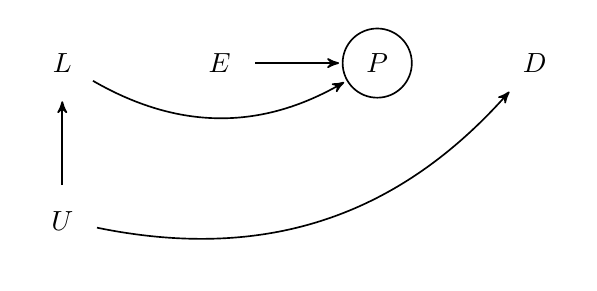
\begin{tikzpicture}[->,>=stealth',shorten >=1pt,auto,node distance=2cm,semithick]
		\node[state,draw = none]         (L)                     {$L$};
		\node[state,draw = none]         (U)    [below of=L]     {$U$};
		\node[state,draw = none]         (E)    [right of=L]     {$E$};
		\node[state,circle]              (P)    [right of=E]     {$P$};
		\node[state,draw = none]         (D)    [right of=P]     {$D$};
		\path (U)   edge  [bend right]   node {} (D)
                    edge                 node {} (L)
              (L)   edge  [bend right]   node {} (P)
              (E)   edge                 node {} (P);
        \end{tikzpicture}
    }
    \caption{}
    \label{fig:f1a}
\end{subfigure}
\begin{subfigure}[b]{0.32\textwidth}
	\centering
	\resizebox{\linewidth}{!}{
		\begin{tikzpicture}[->,>=stealth',shorten >=1pt,auto,node distance=2cm,semithick]
		\node[state,draw = none]         (Us)                    {$U^{*}$};
		\node[state,draw = none]         (E)    [below of=Us]    {$E$};
		\node[state,draw = none]         (U)    [below of=E]     {$U$};
		\node[state,draw = none]         (L)    [right of=E]     {$L$};
		\node[state,circle]              (P)    [right of=L]     {$P$};
		\node[state,draw = none]         (D)    [right of=P]     {$D$};
		\path (Us)  edge                 node {} (E)
		            edge                 node {} (L)
		      (U)   edge  [bend right]   node {} (D)
		            edge                 node {} (L)
		      (L)   edge                 node {} (P);
		\end{tikzpicture}
	}
    \caption{}
	\label{fig:f1b}
\end{subfigure}
\begin{subfigure}[b]{0.32\textwidth}
	\centering
	\resizebox{\linewidth}{!}{
		\begin{tikzpicture}[->,>=latex',shorten >=1pt,auto,node distance=2cm,semithick]
		\node[state,draw = none]         (L)                     {$L$};
		\node[state,draw = none]         (E)    [below of=L]     {$E$};
		\node[state,circle]              (P)    [right of=L]     {$P$};
		\node[]                          (x1)   [right of=P]     {};
		\node[]                          (x2)   [right of=x1]    {};
		\node[state,draw = none]         (D)    [below of=x2]    {$D$};
		
		\path (L)   edge                 node {} (P)
		            edge                 node {} (P)
		      (E)   edge                 node {} (D);
		      
		\draw (L)                    --  node {} ($(E)!0.5!(D)$);
		\end{tikzpicture}
	}
	\caption{}
	\label{fig:f1c}
\end{subfigure}

%\begin{tikzpicture}[->,>=stealth',shorten >=1pt,auto,node distance=2.5cm,semithick]
%
%\node[state,draw = none]         (U*)              {$U^{*}$};
%\node[state,draw = none]         (M) [below of=U*] {$M$};
%\node[state,draw = none]         (E) [right of=M]  {$E$};
%\node[state,circle]              (C) [right of=E]  {$C$};
%\node[state,draw = none]         (O) [right of=C]  {$O$};
%\node[state,draw = none]         (U) [below of=M]  {$U$};

%\path (U*) edge              node {} (E)
%edge              node {} (C)
%(M)  edge [bend right] node {} (C)
%(U)  edge              node {} (M)
%edge [bend right] node {} (O);
%\end{tikzpicture}


		}
	}
	\caption{Structural models of bias due to self-selection or loss to follow-up in prospective cohort studies. A spurious association can manifests when participation $P$ or participation predictors $L$ are colliders on the path between exposure $E$ and outcome $D$. \protect\circled{$P$} indicates conditioning on $P$, which opens a collider, resulting in selection bias. Panel (a) depicts a situation where $L$ and $E$ are independent as long as there is no conditioning on $P$. Inverse probability of participation weighting (IPPW), direct standardization (DS) and multilevel regression and poststratification (MRP), or adjusting for $L$ (AR) reduce this type of selection bias. (b) When $E$ and $L$ share an unobserved common cause, selection bias can only be reduced with IPPW. Panel (c) depicts bias due to effect modification, which can manifest in the absence of unobserved causes or conditioning on a collider. IPPW, DS, and MRP reduce this type of selection bias. (Panels (a) and (b) modified from \cite{Hernan2004-oz}).}
	\label{fig:SelectionBias}
\end{figure}


Figure 1 highlights that bias due to self-selection and loss to follow-up depends on the relationship of variables included in an analysis with each other and with unobserved causes. Therefore, the presence or absence of bias cannot be determined for an entire cohort study that measures different exposures and outcomes. Instead, it has to be determined for each exposure-outcome-pair. Acquiring information about associations that determine selection bias is non-trivial, because \emph{unobserved} common causes of participation predictors and outcome are central. 

Common causes can be of environmental \cite{Johnson2011-wi,Verweij2013-xk} or genetic nature. Without presuming  that common genetic causes carry more weight than environmental factors, we propose to use the more widely reported genetic correlation coefficients ($r_G$) from twin \cite{Tambs2012-km} and genome wide association studies \cite{Bulik-Sullivan2015-er} as an indicator for common unobserved causes. For instance, \citeauthor{Bulik-Sullivan2015-xn} \cite{Bulik-Sullivan2015-xn} report single nucleotide polymorphism (SNP) based genetic correlations of $r_{G_{SNP}}=0.01$ and $0.731$ between education in adulthood and birth-weight or childhood IQ, respectively. Hence, if one uses a study sample that over-represents well-educated mothers to examine associations of maternal depression with birth weight or childhood IQ, the latter association is more likely biased.

The structural approach does not provide an estimate of selection bias--magnitude. Still, the comparison of association estimates obtained with and without correction for self-selection into continued participation can serve as a lower bound estimate of bias. Selection bias can be reduced by adjusting for participation predictors (adjusted regression, AR), by direct standardization with respect to participation predictors (DS \cite{Miettinen1972-vf}) or multilevel regression and poststratification (MRP \cite{Downes2018-oa}), and by weighting participants according to the inverse participation-probability (IPPW \cite{Seaman2013-rj}). While IPPW reduces all types of selection bias displayed in Figure \ref{fig:SelectionBias}, provided participation can be predicted well, DS and MRP reduce bias due to effect modification and structural bias when the exposure does not cause or share a common cause with participation predictors (as in Figures \ref{fig:f1a} and \ref{fig:f1c}). AR only reduces bias in the absence of effect modification and when the exposure does not cause or share a common cause with participation predictors (as in Figure \ref{fig:f1a}). AR, DS, and MRP cannot reduce selection bias when the exposure causes or shares a common cause with participation predictors (as in Figure \ref{fig:f1b}) because conditioning on a collider introduces bias \cite{Cole2010-za}. One disadvantage of IPP weighting is that it relies on a correct specification of the selection model and sufficient data. Therefore, AR should be favored if it is certain that participation predictors do not modify effects and are independent of the exposure in the target population.

In sum, this article proposes to evaluate selection bias in two steps. First, assumptions about common causes in causal models of exposure-outcome association and study participation should be substantiated, for example with estimates of genetic correlations. Second, a lower bound of selection bias magnitude can be estimated by comparing association estimates from IPPW and non-weighted analyses. In the remainder of the article we use associations between child-- and parental characteristics at birth and preschoolers' Attention Deficit Hyperactivity Disorder (ADHD) symptoms in the Norwegian Mother and Child Cohort Study (MoBa) as an example to demonstrate assessment of bias due to self-selection and loss to follow-up in a large prospective cohort study. We estimate the joint effects of self-selection and loss to follow-up by assessing bias in the study sample for which outcome data is available, because both biases are present in longitudinal studies. \emph{Note that in the remainder of the article "bias" refers exclusively to bias due to self-selection and loss to follow-up, and not to any other type of bias.}

\section{Methods}

\subsection{Target population and study sample}

\paragraph{Study sample} MoBa is a prospective population-based pregnancy cohort study conducted by the Norwegian Institute of Public Health  \cite{Magnus2006-jj,Magnus2016-ht}. Participating mothers from all over Norway were recruited during routine ultrasound assessment in week 17 or 18 of their pregnancy in the period from 1999 to 2009. 41\% of the invited women consented to participation. The cohort now includes 114.500 children, 95.200 mothers and 75.200 fathers. The current study is based on version 9 of the quality-assured data files released for research on October 2015. The reported analyses also use information from the Medical Birth Registry (MBRN), a national health registry containing information about all births in Norway \cite{Irgens2000-ra}.

The current analysis uses data from the main inclusion period from January 2001 to December 2009, in which 94373 mothers returned the first MoBa questionnaire around the 20th pregnancy week. Of these 55763 (59\%) also returned the 6th MoBa questionnaire (at child age 3 years). Table \ref{table:age_edu} shows the bivariate distribution of maternal age and education in the MoBa sample and the target population, i.e. women in Norway who gave birth in the sampling period.

\begin{table}[ht]
	\ifthenelse{\boolean{ismanus}}{}{% latex table generated in R 3.4.1 by xtable 1.8-3 package
% Mon Jan 28 15:18:59 2019
\centering
\begin{tabular}{lllrrrrrr}
  \hline
Group & Education & $<$20 & 20-24 & 25-29 & 30-34 & 35-39 & 40-49 & All \\ 
  \hline
MoBa & Elementary & 0.2 & 0.4 & 0.4 & 0.4 & 0.2 & 0.1 & 1.7 \\ 
   & High-school & 0.3 & 6.2 & 9.9 & 8.7 & 4.1 & 0.6 & 29.9 \\ 
   & Bachelor & 0 & 1.8 & 16.7 & 18.0 & 6.2 & 0.8 & 43.7 \\ 
   & Master & 0 & 0.0 & 6.0 & 12.8 & 5.3 & 0.6 & 24.7 \\ 
   & All & 0.6 & 8.4 & 33.1 & 39.9 & 15.9 & 2.1 & 100.0 \\ 
  Population & Elementary & 2 & 5.6 & 5.1 & 3.7 & 1.9 & 0.5 & 18.7 \\ 
   & High-school & 0.3 & 6.8 & 11.9 & 10.3 & 4.6 & 0.8 & 34.7 \\ 
   & Bachelor & 0 & 1.9 & 13.1 & 15.0 & 6.2 & 1.0 & 37.2 \\ 
   & Master & 0 & 0.0 & 1.9 & 4.7 & 2.3 & 0.4 & 9.3 \\ 
   & All & 2.3 & 14.4 & 32.0 & 33.7 & 15.0 & 2.5 & 100.0 \\ 
  Coverage & Elementary & 1.3 & 0.7 & 1.0 & 1.3 & 1.4 & 1.3 & 1.0 \\ 
   & High-school & 12.4 & 10.3 & 9.4 & 9.5 & 10.1 & 9.1 & 9.7 \\ 
   & Bachelor & - & 10.6 & 14.4 & 13.5 & 11.4 & 9.3 & 13.2 \\ 
   & Master & - &  & 35.1 & 30.4 & 25.8 & 19.5 & 29.8 \\ 
   & All & 2.8 & 6.6 & 11.6 & 13.3 & 11.9 & 9.3 & 11.3 \\ 
   \hline
\end{tabular}
}
	\caption{Percent of mothers split by age and education in study sample (n = 54557) and background population (n = 510556), as well as coverage (\% participation) of population subgroups in MoBa. Data for MoBa participants from MoBa and MBRN, population data were obtained from Statistics Norway. While around 30\% of mothers with a Master degree participated, only around 1\% of mothers with only elementary school education or less participated.} 
	\label{table:age_edu}
\end{table}

\paragraph{Participation predictors: Socioeconomic data about the target population}
We obtained aggregated data about maternal age, educational level, and number of children for all women in the target population from Statistics Norway. 


\subsection{Statistical analysis}
R scripts for all analyses steps are available at {\footnotesize https://github.com/gbiele/IPW/tree/master/AnalysisBIPW}. A detailed description of the statistical methods is in the supplementary information.

\paragraph{Investigating unobserved common causes with LD score regression} We calculated genetic correlations between predictors of participation, exposures, and outcome from publicly available summary results of genome wide association studies (GWAS) using linkage disequilibrium (LD) score regressions \cite{Bulik-Sullivan2015-er}. Table \ref{tab:gwas} lists maternal phenotypes for which we obtained GWAS summary statistics. Maternal genetic correlations also inform about common causes of maternal and child phenotypes because mothers and their children share 50\% of their genes.

\paragraph{Outcome, exposures, and adjustment variables} We calculated an ADHD symptom score by summing the responses (Not, Somewhat, or Very often true, coded as 0, 1, 2) to 11 questions about ADHD symptoms that mothers' answered when the child was around 3 years old. Three separate analyses examined the magnitude of selection bias when estimating the association of preschooler ADHD symptoms with (a) birth-related exposures, (b) parental use of legal drugs, and (c) parental mental health including use of illegal drugs. 

Table \ref{table:variables} describes the variables used in the analyses. MoBa assessed parental mental health with short forms of the symptom checklist (SCL5, \cite{Tambs1993-ch}), the lifetime history of depression questionnaire (LTH, \cite{Kendler1993-pf}), and the ADHD Self-Report Scale (ASRS, \cite{Kessler2007-et}). MoBa measured use of illegal drugs (cannabis, ecstasy, amphetamines, cocaine; less than 0.01\% indicated  having used heroin) before or in the pregnancy with Likert scales. As a dimensional measure of illegal drug-use we used ability scores from an item response theory analysis \cite{Rizopoulos2006-bc}. 


\begin{table}[ht]
	\centering
	\ifthenelse{\boolean{ismanus}}{}{\begin{tabular}{lllll}
		\hline
		Type & Variable & Description & Source & Used in\\ 
		\hline
		\multicolumn{5}{l}{Outcome:} \\
		& child ADHD & SS ADHD symptom ratings & Q6 & IAU\\ 
		\multicolumn{5}{l}{Exposures, birth-related:} \\
		& small f. gest. age & 1 = among 5\% lightest in gest. wk. & MBRN & IAU\\ 
		& preterm & 1 = birthweek $<$ 37 & MBRN & IAU\\ 
		\multicolumn{5}{l}{Exposures, Parental mental health:} \\
		& m. drug use & used any drug 1 = yes, no = 0 & Q1 & IAU\\ 
		& m. drug use score & ability score from IRT model & Q1 & IAU\\ 
		& m. LTH & SS Lifetime History of Depression & Q1 & IAU\\ 
		& m. SCL5 & SS Symptom Check list & Q1 & IAU\\ 
		& p. drug use & used any drug 1 = yes, no = 0 & QF & IAU\\ 
		& p. drug use score & ability score from IRT model & QF & IAU\\ 
		\multicolumn{5}{l}{Exposures, parental use of legal drugs:} \\
		& m. smoking & smoking in pregn.: 1 = yes, 0 = no & Q1 & IAU\\ 
		& m. num. cigarettes & cigarettes per day in pregnancy & Q1 & IAU\\ 
		& m. alc. freq. & in pregnancy, 3 ordered categories & Q1 & IAU\\ 
		& m. eff. units. alc. & effective units of alcohol & Q1 & IAU\\ 
		& p. smoking & smoking, 1 = yes, 0 = no & QF & IAU\\ 
		& p. num. cigarettes & cigarettes per day & QF & IAU\\ 
		& p. alc. freq. & drinking per week & QF & IAU\\ 
		& p. typ. units. alc. & typical number of units alcohol  & QF & IAU\\
		\multicolumn{5}{l}{Adjustment variables:} \\ 
		& child sex & 0 = boys, 1 = girls & MBRN & IA\\ 
		& m. BMI deviat. & log(BMI/mode of BMI) & Q1 & IA \\ 
		& m. ADHD & SS ASRS & Q6 & IA \\ 
		& p. ADHD & SS ASRS & QF & IA \\
		& p. age & 8 ordered categories & QF & IA \\ 
		& p. education & 4 ordered categories & QF & IA \\ 
		\multicolumn{5}{l}{Participation predictors:} \\ 
		& m. education & 4 ordered categories & Q1  & I$_S$A\\ 
		& m. age & 6 ordered categories & Q1  & I$_S$A\\ 
		& Parity & number of children born & MBRN  & I$_S$A\\ 
		\hline
	\end{tabular}}
	\caption{Description of variables and their use.
		\newline m. = maternal, p. = paternal, Q = MoBa questionnaires, Q1 = at pregnancy week 17, QF = for fathers' (week 20), Q6 = at child age 3, MBRN = Medical Birth Registry of Norway, SS = sum score. All continuous and count variables except parity scaled to a mean of zero and a standard deviation of one. I = used in IPPW model, A = AR model, U = UR model, I$_S$ in selection model for IPPWs calculation, not for adjustment in IPPW model.} 
	\label{table:variables}
\end{table}


All presented analyses used participants for which at least 50\% of the analysis variables were available. We created 20 multiply imputed data sets through multiple imputation by chained equations as implemented in the R package mi \cite{Su2011-he}. 

\paragraph{IPPWs and bias estimation}

We calculated stabilized inverse probability weights using tabulated data about education, age and number of children for all birth giving mothers in Norway in the sampling period of MoBa. Because we rely on tabulated data, we used a binomial regression to estimate participation probabilities for population subgroups. We used a Bayesian hierarchical regression with random intercepts and slopes for the effect of age in subgroups defined by education and parity, in order to estimate effects of age also in small sub-groups reliably.


The estimation of a lower bound for bias involves estimating an IPPW and alternative regression models. The IPPW model estimates weighted and adjusted exposure outcome associations. The AR model, following typical practice for the analysis of cohort studies, adjusts for participation predictors instead of using IPPWs. The unadjusted regression (UR) does no adjustment and uses no IPPWs (c.f. Tables \ref{table:variables} and \ref{tab:regmodels}). To account for covariation of regression weights, we fit the three models (IPPW, AR, UR) simultaneously in a Bayesian framework, and define regression weights for exposures in the AR and UR models as weights from the IPPW model plus difference terms. Because ADHD sum scores are constraint between 0 and 22, we used a beta binomial regression model and report associations as average marginal effects (AMEs).

Based on this analysis model, we calculated the lower bound bias estimate as the difference between AMEs from the IPPW and AR or UR models, respectively. We standardised the lower bound bias by dividing the difference with either the standard deviation or the mean of the posterior distribution of the IPPW estimate (c.f. \cite{Austin2009-xk,Nilsen2009-ci}). The latter approach appeals to the intuition that bias is problematic if the comparison standard is known with high precision/certainty, whereas the former appeals to the intuition that bias is problematic if it has a large deviation from the comparison standard. 

To test for bias, we check how much of the posterior distribution of the bias estimate lies within a region of practical equivalence (ROPE, dashed vertical lines in Figure \ref{fig:estimates}), i.e., a bias magnitude that is for practical purposes equivalent to zero \cite{Mascha2011-um}. Earlier research defined deviations of larger than 30\% or 40\% of the standard deviation or mean of the comparison standard as problematic \cite{Stuart2010-cj,Nohr2006-uf}. Here, we consider values of less than 0.5 standardised AME differences as practically equivalent with zero. To obtain a measure of risk for bias we calculate the log of the ratio of the posterior distribution inside and outside the ROPE, $log(RR_b)$. For example, a $log(RR_b)$ of -1.6 (3) means that the lower bound bias estimate is five (20) times as likely to lie outside (inside) the ROPE.

Regression analyses were performed with custom models implemented in the probabilistic programming language Stan \cite{Stan_Development_Team2017-lp} and fit via RStan \cite{Stan_Development_Team_2018-rs}.

\section{Results}

Statistics Norway recorded 510\,561 women who became mothers in the period from 2001 to 2009. In the same period, 94\,373 mothers returned the first MoBa questionnaire. Of these, 55\,763 also returned the sixth questionnaire,  which was sent out when  children were 3 years old. 54\,557 returned questionnaires with fewer than 50\% missing data among the variables of interest. The study sample used for the reported analysis constitutes around 11\% of the target population.

\subsection*{Socio-demographic composition of study sample and population}
 Mothers with elementary school education or less constitute around 18.7\% of the target population and 1.7\% of the MoBa sample (c.f. Table \ref{table:age_edu}). 16.6\% of mothers in the target population were younger than 25, compared to around 9.1\% in the study sample. Accordingly, the participation rates vary between population subgroups: 29.7\% of mothers in the target population with a master's degree are in the study sample, and around 1\% of mothers with elementary school education. For parity, the difference between study sample and target population is less pronounced. The percentages of women in the target population (study sample) who had previously 0, 1, 2, or 3 or more children are 41.8 (50.9), 36.3 (32.5), 16.1 (13.9), 2.8 (5.8), respectively. Hence, the study sample over-represents mothers of firstborn children and under-represents those with more than two children.

\subsection*{Inverse probability weights}
The hierarchical binomial model captured participation well, as indicated by a correlation of $r=0.99$ between modelled and observed participation rates (see Figure \ref{fig:IPW}). Mothers' education was the key variable to predict participation. Stabilized weights ranged between on average 0.31 and 21.36. The largest weights were for mothers with only elementary school education, and the smallest for mothers with a master's degree. We chose not to trim extreme weights, because this would result in improper weighting of the study sample. While some weights are very large, the associated population subgroups are typically represented with more than  100 children in the study sample.

\subsection*{Unobserved common causes}
Genetic correlation results shown in Figure \ref{fig:rg} indicate unobserved common causes of participation predictors and outcome or exposures, respectively. For example, genes associated with "age at first birth" or "years of education" are also (negatively) associated with ADHD, maternal mental health, or smoking. The estimated SNP based genetic heritability of the investigate phenotypes is typically not high, and often below 10\%.

\begin{figure}
	\begin{center}
		\ifthenelse{\boolean{ismanus}}{}{% Created by tikzDevice version 0.12 on 2019-01-25 19:24:20
% !TEX encoding = UTF-8 Unicode
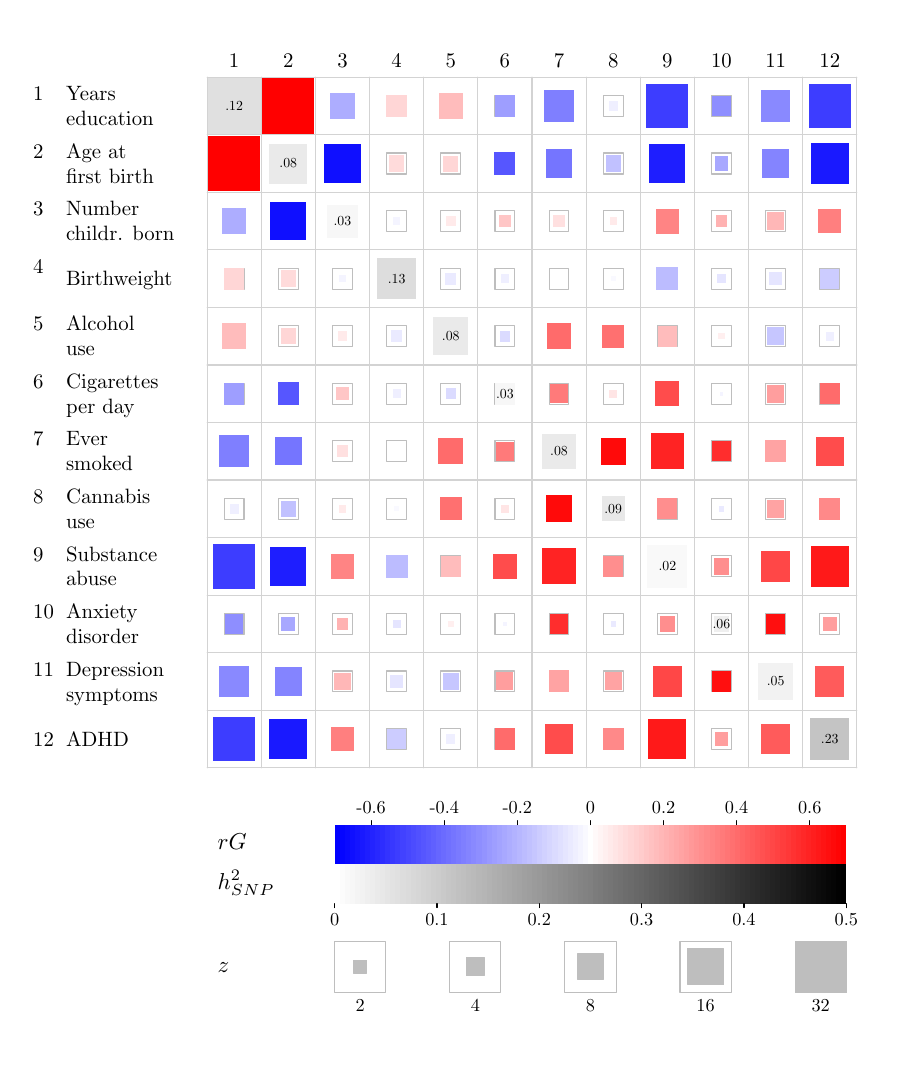
\begin{tikzpicture}[x=1pt,y=1pt]
\definecolor{fillColor}{RGB}{255,255,255}
\path[use as bounding box,fill=fillColor,fill opacity=0.00] (0,0) rectangle (312.98,369.89);
\begin{scope}
\path[clip] ( 55.44, 92.47) rectangle (309.02,361.97);
\definecolor{drawColor}{RGB}{190,190,190}
\definecolor{fillColor}{RGB}{255,255,255}

\path[draw=drawColor,line width= 0.4pt,line join=round,line cap=round,fill=fillColor] (110.19,317.01) rectangle (117.31,324.58);
\definecolor{fillColor}{RGB}{15,15,255}

\path[fill=fillColor] (107.18,313.82) rectangle (120.31,327.77);
\definecolor{fillColor}{RGB}{255,255,255}

\path[draw=drawColor,line width= 0.4pt,line join=round,line cap=round,fill=fillColor] ( 90.62,296.21) rectangle ( 97.74,303.78);
\definecolor{fillColor}{RGB}{15,15,255}

\path[fill=fillColor] ( 87.62,293.02) rectangle (100.75,306.98);
\definecolor{fillColor}{RGB}{255,255,255}

\path[draw=drawColor,line width= 0.4pt,line join=round,line cap=round,fill=fillColor] (286.28,317.01) rectangle (293.41,324.58);
\definecolor{fillColor}{RGB}{25,25,255}

\path[fill=fillColor] (283.01,313.53) rectangle (296.68,328.06);
\definecolor{fillColor}{RGB}{255,255,255}

\path[draw=drawColor,line width= 0.4pt,line join=round,line cap=round,fill=fillColor] ( 90.62,109.06) rectangle ( 97.74,116.64);
\definecolor{fillColor}{RGB}{25,25,255}

\path[fill=fillColor] ( 87.35,105.59) rectangle (101.02,120.11);
\definecolor{fillColor}{RGB}{255,255,255}

\path[draw=drawColor,line width= 0.4pt,line join=round,line cap=round,fill=fillColor] (227.58,317.01) rectangle (234.71,324.58);
\definecolor{fillColor}{RGB}{30,30,255}

\path[fill=fillColor] (224.62,313.86) rectangle (237.67,327.73);
\definecolor{fillColor}{RGB}{255,255,255}

\path[draw=drawColor,line width= 0.4pt,line join=round,line cap=round,fill=fillColor] ( 90.62,171.45) rectangle ( 97.74,179.02);
\definecolor{fillColor}{RGB}{30,30,255}

\path[fill=fillColor] ( 87.66,168.30) rectangle (100.71,182.17);
\definecolor{fillColor}{RGB}{255,255,255}

\path[draw=drawColor,line width= 0.4pt,line join=round,line cap=round,fill=fillColor] (286.28,337.80) rectangle (293.41,345.37);
\definecolor{fillColor}{RGB}{61,61,255}

\path[fill=fillColor] (282.21,333.48) rectangle (297.48,349.70);
\definecolor{fillColor}{RGB}{255,255,255}

\path[draw=drawColor,line width= 0.4pt,line join=round,line cap=round,fill=fillColor] (227.58,337.80) rectangle (234.71,345.37);
\definecolor{fillColor}{RGB}{61,61,255}

\path[fill=fillColor] (223.58,333.55) rectangle (238.71,349.62);
\definecolor{fillColor}{RGB}{255,255,255}

\path[draw=drawColor,line width= 0.4pt,line join=round,line cap=round,fill=fillColor] ( 71.05,109.06) rectangle ( 78.18,116.64);
\definecolor{fillColor}{RGB}{61,61,255}

\path[fill=fillColor] ( 66.98,104.74) rectangle ( 82.25,120.96);
\definecolor{fillColor}{RGB}{255,255,255}

\path[draw=drawColor,line width= 0.4pt,line join=round,line cap=round,fill=fillColor] ( 71.05,171.45) rectangle ( 78.18,179.02);
\definecolor{fillColor}{RGB}{61,61,255}

\path[fill=fillColor] ( 67.05,167.20) rectangle ( 82.18,183.27);
\definecolor{fillColor}{RGB}{255,255,255}

\path[draw=drawColor,line width= 0.4pt,line join=round,line cap=round,fill=fillColor] (168.88,317.01) rectangle (176.01,324.58);
\definecolor{fillColor}{RGB}{86,86,255}

\path[fill=fillColor] (168.63,316.73) rectangle (176.27,324.85);
\definecolor{fillColor}{RGB}{255,255,255}

\path[draw=drawColor,line width= 0.4pt,line join=round,line cap=round,fill=fillColor] ( 90.62,233.83) rectangle ( 97.74,241.40);
\definecolor{fillColor}{RGB}{86,86,255}

\path[fill=fillColor] ( 90.36,233.55) rectangle ( 98.00,241.68);
\definecolor{fillColor}{RGB}{255,255,255}

\path[draw=drawColor,line width= 0.4pt,line join=round,line cap=round,fill=fillColor] (188.45,317.01) rectangle (195.58,324.58);
\definecolor{fillColor}{RGB}{117,117,255}

\path[fill=fillColor] (187.19,315.66) rectangle (196.84,325.92);
\definecolor{fillColor}{RGB}{255,255,255}

\path[draw=drawColor,line width= 0.4pt,line join=round,line cap=round,fill=fillColor] ( 90.62,213.04) rectangle ( 97.74,220.61);
\definecolor{fillColor}{RGB}{117,117,255}

\path[fill=fillColor] ( 89.36,211.69) rectangle ( 99.01,221.95);
\definecolor{fillColor}{RGB}{255,255,255}

\path[draw=drawColor,line width= 0.4pt,line join=round,line cap=round,fill=fillColor] ( 71.05,213.04) rectangle ( 78.18,220.61);
\definecolor{fillColor}{RGB}{127,127,255}

\path[fill=fillColor] ( 69.24,211.11) rectangle ( 79.99,222.54);
\definecolor{fillColor}{RGB}{255,255,255}

\path[draw=drawColor,line width= 0.4pt,line join=round,line cap=round,fill=fillColor] (188.45,337.80) rectangle (195.58,345.37);
\definecolor{fillColor}{RGB}{127,127,255}

\path[fill=fillColor] (186.64,335.87) rectangle (197.39,347.30);
\definecolor{fillColor}{RGB}{255,255,255}

\path[draw=drawColor,line width= 0.4pt,line join=round,line cap=round,fill=fillColor] (266.72,317.01) rectangle (273.84,324.58);
\definecolor{fillColor}{RGB}{132,132,255}

\path[fill=fillColor] (265.42,315.63) rectangle (275.14,325.96);
\definecolor{fillColor}{RGB}{255,255,255}

\path[draw=drawColor,line width= 0.4pt,line join=round,line cap=round,fill=fillColor] ( 90.62,129.86) rectangle ( 97.74,137.43);
\definecolor{fillColor}{RGB}{132,132,255}

\path[fill=fillColor] ( 89.32,128.48) rectangle ( 99.04,138.81);
\definecolor{fillColor}{RGB}{255,255,255}

\path[draw=drawColor,line width= 0.4pt,line join=round,line cap=round,fill=fillColor] (266.72,337.80) rectangle (273.84,345.37);
\definecolor{fillColor}{RGB}{137,137,255}

\path[fill=fillColor] (264.94,335.92) rectangle (275.61,347.26);
\definecolor{fillColor}{RGB}{255,255,255}

\path[draw=drawColor,line width= 0.4pt,line join=round,line cap=round,fill=fillColor] ( 71.05,129.86) rectangle ( 78.18,137.43);
\definecolor{fillColor}{RGB}{137,137,255}

\path[fill=fillColor] ( 69.28,127.98) rectangle ( 79.95,139.31);
\definecolor{fillColor}{RGB}{255,255,255}

\path[draw=drawColor,line width= 0.4pt,line join=round,line cap=round,fill=fillColor] (247.15,337.80) rectangle (254.27,345.37);
\definecolor{fillColor}{RGB}{142,142,255}

\path[fill=fillColor] (247.37,338.04) rectangle (254.05,345.13);
\definecolor{fillColor}{RGB}{255,255,255}

\path[draw=drawColor,line width= 0.4pt,line join=round,line cap=round,fill=fillColor] ( 71.05,150.65) rectangle ( 78.18,158.22);
\definecolor{fillColor}{RGB}{142,142,255}

\path[fill=fillColor] ( 71.28,150.89) rectangle ( 77.95,157.99);
\definecolor{fillColor}{RGB}{255,255,255}

\path[draw=drawColor,line width= 0.4pt,line join=round,line cap=round,fill=fillColor] (168.88,337.80) rectangle (176.01,345.37);
\definecolor{fillColor}{RGB}{158,158,255}

\path[fill=fillColor] (168.76,337.67) rectangle (176.13,345.51);
\definecolor{fillColor}{RGB}{255,255,255}

\path[draw=drawColor,line width= 0.4pt,line join=round,line cap=round,fill=fillColor] ( 71.05,233.83) rectangle ( 78.18,241.40);
\definecolor{fillColor}{RGB}{158,158,255}

\path[fill=fillColor] ( 70.93,233.70) rectangle ( 78.30,241.53);
\definecolor{fillColor}{RGB}{255,255,255}

\path[draw=drawColor,line width= 0.4pt,line join=round,line cap=round,fill=fillColor] (247.15,317.01) rectangle (254.27,324.58);
\definecolor{fillColor}{RGB}{168,168,255}

\path[fill=fillColor] (248.22,318.15) rectangle (253.20,323.44);
\definecolor{fillColor}{RGB}{255,255,255}

\path[draw=drawColor,line width= 0.4pt,line join=round,line cap=round,fill=fillColor] ( 90.62,150.65) rectangle ( 97.74,158.22);
\definecolor{fillColor}{RGB}{168,168,255}

\path[fill=fillColor] ( 91.69,151.79) rectangle ( 96.67,157.09);
\definecolor{fillColor}{RGB}{255,255,255}

\path[draw=drawColor,line width= 0.4pt,line join=round,line cap=round,fill=fillColor] ( 71.05,296.21) rectangle ( 78.18,303.78);
\definecolor{fillColor}{RGB}{173,173,255}

\path[fill=fillColor] ( 70.24,295.35) rectangle ( 78.99,304.65);
\definecolor{fillColor}{RGB}{255,255,255}

\path[draw=drawColor,line width= 0.4pt,line join=round,line cap=round,fill=fillColor] (110.19,337.80) rectangle (117.31,345.37);
\definecolor{fillColor}{RGB}{173,173,255}

\path[fill=fillColor] (109.37,336.94) rectangle (118.12,346.24);
\definecolor{fillColor}{RGB}{255,255,255}

\path[draw=drawColor,line width= 0.4pt,line join=round,line cap=round,fill=fillColor] (227.58,275.42) rectangle (234.71,282.99);
\definecolor{fillColor}{RGB}{188,188,255}

\path[fill=fillColor] (227.21,275.03) rectangle (235.08,283.38);
\definecolor{fillColor}{RGB}{255,255,255}

\path[draw=drawColor,line width= 0.4pt,line join=round,line cap=round,fill=fillColor] (129.75,171.45) rectangle (136.88,179.02);
\definecolor{fillColor}{RGB}{188,188,255}

\path[fill=fillColor] (129.38,171.05) rectangle (137.25,179.41);
\definecolor{fillColor}{RGB}{255,255,255}

\path[draw=drawColor,line width= 0.4pt,line join=round,line cap=round,fill=fillColor] (208.02,317.01) rectangle (215.14,324.58);
\definecolor{fillColor}{RGB}{193,193,255}

\path[fill=fillColor] (208.85,317.89) rectangle (214.31,323.70);
\definecolor{fillColor}{RGB}{255,255,255}

\path[draw=drawColor,line width= 0.4pt,line join=round,line cap=round,fill=fillColor] ( 90.62,192.24) rectangle ( 97.74,199.81);
\definecolor{fillColor}{RGB}{193,193,255}

\path[fill=fillColor] ( 91.45,193.12) rectangle ( 96.91,198.93);
\definecolor{fillColor}{RGB}{255,255,255}

\path[draw=drawColor,line width= 0.4pt,line join=round,line cap=round,fill=fillColor] (149.32,129.86) rectangle (156.44,137.43);
\definecolor{fillColor}{RGB}{198,198,255}

\path[fill=fillColor] (149.92,130.50) rectangle (155.84,136.79);
\definecolor{fillColor}{RGB}{255,255,255}

\path[draw=drawColor,line width= 0.4pt,line join=round,line cap=round,fill=fillColor] (266.72,254.62) rectangle (273.84,262.20);
\definecolor{fillColor}{RGB}{198,198,255}

\path[fill=fillColor] (267.32,255.26) rectangle (273.24,261.56);
\definecolor{fillColor}{RGB}{255,255,255}

\path[draw=drawColor,line width= 0.4pt,line join=round,line cap=round,fill=fillColor] (286.28,275.42) rectangle (293.41,282.99);
\definecolor{fillColor}{RGB}{204,204,255}

\path[fill=fillColor] (286.48,275.62) rectangle (293.22,282.79);
\definecolor{fillColor}{RGB}{255,255,255}

\path[draw=drawColor,line width= 0.4pt,line join=round,line cap=round,fill=fillColor] (129.75,109.06) rectangle (136.88,116.64);
\definecolor{fillColor}{RGB}{204,204,255}

\path[fill=fillColor] (129.94,109.27) rectangle (136.68,116.43);
\definecolor{fillColor}{RGB}{255,255,255}

\path[draw=drawColor,line width= 0.4pt,line join=round,line cap=round,fill=fillColor] (149.32,233.83) rectangle (156.44,241.40);
\definecolor{fillColor}{RGB}{219,219,255}

\path[fill=fillColor] (151.04,235.66) rectangle (154.72,239.58);
\definecolor{fillColor}{RGB}{255,255,255}

\path[draw=drawColor,line width= 0.4pt,line join=round,line cap=round,fill=fillColor] (168.88,254.62) rectangle (176.01,262.20);
\definecolor{fillColor}{RGB}{219,219,255}

\path[fill=fillColor] (170.60,256.45) rectangle (174.29,260.37);
\definecolor{fillColor}{RGB}{255,255,255}

\path[draw=drawColor,line width= 0.4pt,line join=round,line cap=round,fill=fillColor] (129.75,150.65) rectangle (136.88,158.22);
\definecolor{fillColor}{RGB}{229,229,255}

\path[fill=fillColor] (131.87,152.90) rectangle (134.76,155.98);
\definecolor{fillColor}{RGB}{255,255,255}

\path[draw=drawColor,line width= 0.4pt,line join=round,line cap=round,fill=fillColor] (129.75,129.86) rectangle (136.88,137.43);
\definecolor{fillColor}{RGB}{229,229,255}

\path[fill=fillColor] (131.00,131.18) rectangle (135.63,136.11);
\definecolor{fillColor}{RGB}{255,255,255}

\path[draw=drawColor,line width= 0.4pt,line join=round,line cap=round,fill=fillColor] (247.15,275.42) rectangle (254.27,282.99);
\definecolor{fillColor}{RGB}{229,229,255}

\path[fill=fillColor] (249.26,277.67) rectangle (252.16,280.74);
\definecolor{fillColor}{RGB}{255,255,255}

\path[draw=drawColor,line width= 0.4pt,line join=round,line cap=round,fill=fillColor] (266.72,275.42) rectangle (273.84,282.99);
\definecolor{fillColor}{RGB}{229,229,255}

\path[fill=fillColor] (267.96,276.74) rectangle (272.60,281.67);
\definecolor{fillColor}{RGB}{255,255,255}

\path[draw=drawColor,line width= 0.4pt,line join=round,line cap=round,fill=fillColor] (149.32,275.42) rectangle (156.44,282.99);
\definecolor{fillColor}{RGB}{234,234,255}

\path[fill=fillColor] (150.83,277.02) rectangle (154.93,281.39);
\definecolor{fillColor}{RGB}{255,255,255}

\path[draw=drawColor,line width= 0.4pt,line join=round,line cap=round,fill=fillColor] (208.02,150.65) rectangle (215.14,158.22);
\definecolor{fillColor}{RGB}{234,234,255}

\path[fill=fillColor] (210.63,153.43) rectangle (212.53,155.45);
\definecolor{fillColor}{RGB}{255,255,255}

\path[draw=drawColor,line width= 0.4pt,line join=round,line cap=round,fill=fillColor] (129.75,254.62) rectangle (136.88,262.20);
\definecolor{fillColor}{RGB}{234,234,255}

\path[fill=fillColor] (131.26,256.23) rectangle (135.37,260.59);
\definecolor{fillColor}{RGB}{255,255,255}

\path[draw=drawColor,line width= 0.4pt,line join=round,line cap=round,fill=fillColor] (247.15,192.24) rectangle (254.27,199.81);
\definecolor{fillColor}{RGB}{234,234,255}

\path[fill=fillColor] (249.76,195.02) rectangle (251.66,197.04);
\definecolor{fillColor}{RGB}{255,255,255}

\path[draw=drawColor,line width= 0.4pt,line join=round,line cap=round,fill=fillColor] (149.32,109.06) rectangle (156.44,116.64);
\definecolor{fillColor}{RGB}{239,239,255}

\path[fill=fillColor] (151.33,111.20) rectangle (154.43,114.50);
\definecolor{fillColor}{RGB}{255,255,255}

\path[draw=drawColor,line width= 0.4pt,line join=round,line cap=round,fill=fillColor] (208.02,337.80) rectangle (215.14,345.37);
\definecolor{fillColor}{RGB}{239,239,255}

\path[fill=fillColor] (209.90,339.80) rectangle (213.26,343.37);
\definecolor{fillColor}{RGB}{255,255,255}

\path[draw=drawColor,line width= 0.4pt,line join=round,line cap=round,fill=fillColor] (168.88,275.42) rectangle (176.01,282.99);
\definecolor{fillColor}{RGB}{239,239,255}

\path[fill=fillColor] (170.96,277.62) rectangle (173.93,280.78);
\definecolor{fillColor}{RGB}{255,255,255}

\path[draw=drawColor,line width= 0.4pt,line join=round,line cap=round,fill=fillColor] (286.28,254.62) rectangle (293.41,262.20);
\definecolor{fillColor}{RGB}{239,239,255}

\path[fill=fillColor] (288.30,256.76) rectangle (291.39,260.06);
\definecolor{fillColor}{RGB}{255,255,255}

\path[draw=drawColor,line width= 0.4pt,line join=round,line cap=round,fill=fillColor] ( 71.05,192.24) rectangle ( 78.18,199.81);
\definecolor{fillColor}{RGB}{239,239,255}

\path[fill=fillColor] ( 72.93,194.24) rectangle ( 76.30,197.81);
\definecolor{fillColor}{RGB}{255,255,255}

\path[draw=drawColor,line width= 0.4pt,line join=round,line cap=round,fill=fillColor] (129.75,233.83) rectangle (136.88,241.40);
\definecolor{fillColor}{RGB}{239,239,255}

\path[fill=fillColor] (131.83,236.04) rectangle (134.80,239.20);
\definecolor{fillColor}{RGB}{255,255,255}

\path[draw=drawColor,line width= 0.4pt,line join=round,line cap=round,fill=fillColor] (129.75,296.21) rectangle (136.88,303.78);
\definecolor{fillColor}{RGB}{244,244,255}

\path[fill=fillColor] (132.01,298.61) rectangle (134.62,301.38);
\definecolor{fillColor}{RGB}{255,255,255}

\path[draw=drawColor,line width= 0.4pt,line join=round,line cap=round,fill=fillColor] (168.88,150.65) rectangle (176.01,158.22);
\definecolor{fillColor}{RGB}{244,244,255}

\path[fill=fillColor] (171.75,153.69) rectangle (173.15,155.18);
\definecolor{fillColor}{RGB}{255,255,255}

\path[draw=drawColor,line width= 0.4pt,line join=round,line cap=round,fill=fillColor] (110.19,275.42) rectangle (117.31,282.99);
\definecolor{fillColor}{RGB}{244,244,255}

\path[fill=fillColor] (112.44,277.82) rectangle (115.05,280.59);
\definecolor{fillColor}{RGB}{255,255,255}

\path[draw=drawColor,line width= 0.4pt,line join=round,line cap=round,fill=fillColor] (247.15,233.83) rectangle (254.27,241.40);
\definecolor{fillColor}{RGB}{244,244,255}

\path[fill=fillColor] (250.01,236.87) rectangle (251.41,238.36);
\definecolor{fillColor}{RGB}{255,255,255}

\path[draw=drawColor,line width= 0.4pt,line join=round,line cap=round,fill=fillColor] (208.02,275.42) rectangle (215.14,282.99);
\definecolor{fillColor}{RGB}{249,249,255}

\path[fill=fillColor] (210.68,278.25) rectangle (212.48,280.16);
\definecolor{fillColor}{RGB}{255,255,255}

\path[draw=drawColor,line width= 0.4pt,line join=round,line cap=round,fill=fillColor] (129.75,192.24) rectangle (136.88,199.81);
\definecolor{fillColor}{RGB}{249,249,255}

\path[fill=fillColor] (132.42,195.07) rectangle (134.21,196.98);
\definecolor{fillColor}{RGB}{255,255,255}

\path[draw=drawColor,line width= 0.4pt,line join=round,line cap=round,fill=fillColor] (129.75,213.04) rectangle (136.88,220.61);

\path[fill=fillColor] (132.63,216.09) rectangle (134.00,217.55);

\path[draw=drawColor,line width= 0.4pt,line join=round,line cap=round,fill=fillColor] (188.45,275.42) rectangle (195.58,282.99);

\path[fill=fillColor] (191.33,278.47) rectangle (192.70,279.94);

\path[draw=drawColor,line width= 0.4pt,line join=round,line cap=round,fill=fillColor] (227.58,171.45) rectangle (234.71,179.02);
\definecolor{fillColor}{RGB}{249,249,249}

\path[fill=fillColor] (223.94,167.58) rectangle (238.35,182.89);
\definecolor{drawColor}{RGB}{0,0,0}

\node[text=drawColor,anchor=base,inner sep=0pt, outer sep=0pt, scale=  0.50] at (231.15,173.65) {.02};
\definecolor{drawColor}{RGB}{190,190,190}
\definecolor{fillColor}{RGB}{255,255,255}

\path[draw=drawColor,line width= 0.4pt,line join=round,line cap=round,fill=fillColor] (168.88,233.83) rectangle (176.01,241.40);
\definecolor{fillColor}{gray}{0.97}

\path[fill=fillColor] (168.75,233.68) rectangle (176.15,241.55);
\definecolor{drawColor}{RGB}{0,0,0}

\node[text=drawColor,anchor=base,inner sep=0pt, outer sep=0pt, scale=  0.50] at (172.45,236.03) {.03};
\definecolor{drawColor}{RGB}{190,190,190}
\definecolor{fillColor}{RGB}{255,255,255}

\path[draw=drawColor,line width= 0.4pt,line join=round,line cap=round,fill=fillColor] (110.19,296.21) rectangle (117.31,303.78);
\definecolor{fillColor}{gray}{0.97}

\path[fill=fillColor] (108.13,294.03) rectangle (119.36,305.96);
\definecolor{drawColor}{RGB}{0,0,0}

\node[text=drawColor,anchor=base,inner sep=0pt, outer sep=0pt, scale=  0.50] at (113.75,298.41) {.03};
\definecolor{drawColor}{RGB}{190,190,190}
\definecolor{fillColor}{RGB}{255,255,255}

\path[draw=drawColor,line width= 0.4pt,line join=round,line cap=round,fill=fillColor] (149.32,150.65) rectangle (156.44,158.22);
\definecolor{fillColor}{RGB}{255,239,239}

\path[fill=fillColor] (151.78,153.27) rectangle (153.98,155.61);
\definecolor{fillColor}{RGB}{255,255,255}

\path[draw=drawColor,line width= 0.4pt,line join=round,line cap=round,fill=fillColor] (247.15,254.62) rectangle (254.27,262.20);
\definecolor{fillColor}{RGB}{255,239,239}

\path[fill=fillColor] (249.61,257.24) rectangle (251.82,259.58);
\definecolor{fillColor}{RGB}{255,255,255}

\path[draw=drawColor,line width= 0.4pt,line join=round,line cap=round,fill=fillColor] (266.72,129.86) rectangle (273.84,137.43);
\definecolor{fillColor}{gray}{0.95}

\path[fill=fillColor] (263.92,126.88) rectangle (276.64,140.40);
\definecolor{drawColor}{RGB}{0,0,0}

\node[text=drawColor,anchor=base,inner sep=0pt, outer sep=0pt, scale=  0.50] at (270.28,132.06) {.05};
\definecolor{drawColor}{RGB}{190,190,190}
\definecolor{fillColor}{RGB}{255,255,255}

\path[draw=drawColor,line width= 0.4pt,line join=round,line cap=round,fill=fillColor] (208.02,296.21) rectangle (215.14,303.78);
\definecolor{fillColor}{RGB}{255,234,234}

\path[fill=fillColor] (210.29,298.63) rectangle (212.87,301.37);
\definecolor{fillColor}{RGB}{255,255,255}

\path[draw=drawColor,line width= 0.4pt,line join=round,line cap=round,fill=fillColor] (110.19,192.24) rectangle (117.31,199.81);
\definecolor{fillColor}{RGB}{255,234,234}

\path[fill=fillColor] (112.46,194.66) rectangle (115.04,197.40);
\definecolor{fillColor}{RGB}{255,255,255}

\path[draw=drawColor,line width= 0.4pt,line join=round,line cap=round,fill=fillColor] (149.32,296.21) rectangle (156.44,303.78);
\definecolor{fillColor}{RGB}{255,234,234}

\path[fill=fillColor] (151.10,298.11) rectangle (154.66,301.89);
\definecolor{fillColor}{RGB}{255,255,255}

\path[draw=drawColor,line width= 0.4pt,line join=round,line cap=round,fill=fillColor] (110.19,254.62) rectangle (117.31,262.20);
\definecolor{fillColor}{RGB}{255,234,234}

\path[fill=fillColor] (111.97,256.52) rectangle (115.53,260.30);
\definecolor{fillColor}{RGB}{255,255,255}

\path[draw=drawColor,line width= 0.4pt,line join=round,line cap=round,fill=fillColor] (247.15,150.65) rectangle (254.27,158.22);
\definecolor{fillColor}{RGB}{239,239,239}

\path[fill=fillColor] (247.88,151.43) rectangle (253.54,157.45);
\definecolor{drawColor}{RGB}{0,0,0}

\node[text=drawColor,anchor=base,inner sep=0pt, outer sep=0pt, scale=  0.50] at (250.71,152.85) {.06};
\definecolor{drawColor}{RGB}{190,190,190}
\definecolor{fillColor}{RGB}{255,255,255}

\path[draw=drawColor,line width= 0.4pt,line join=round,line cap=round,fill=fillColor] (208.02,233.83) rectangle (215.14,241.40);
\definecolor{fillColor}{RGB}{255,229,229}

\path[fill=fillColor] (210.23,236.18) rectangle (212.93,239.05);
\definecolor{fillColor}{RGB}{255,255,255}

\path[draw=drawColor,line width= 0.4pt,line join=round,line cap=round,fill=fillColor] (168.88,192.24) rectangle (176.01,199.81);
\definecolor{fillColor}{RGB}{255,229,229}

\path[fill=fillColor] (171.10,194.60) rectangle (173.79,197.46);
\definecolor{fillColor}{RGB}{255,255,255}

\path[draw=drawColor,line width= 0.4pt,line join=round,line cap=round,fill=fillColor] (188.45,213.04) rectangle (195.58,220.61);
\definecolor{fillColor}{RGB}{234,234,234}

\path[fill=fillColor] (186.00,210.43) rectangle (198.03,223.22);
\definecolor{drawColor}{RGB}{0,0,0}

\node[text=drawColor,anchor=base,inner sep=0pt, outer sep=0pt, scale=  0.50] at (192.01,215.23) {.08};
\definecolor{drawColor}{RGB}{190,190,190}
\definecolor{fillColor}{RGB}{255,255,255}

\path[draw=drawColor,line width= 0.4pt,line join=round,line cap=round,fill=fillColor] (188.45,296.21) rectangle (195.58,303.78);
\definecolor{fillColor}{RGB}{255,224,224}

\path[fill=fillColor] (190.00,297.86) rectangle (194.03,302.14);
\definecolor{fillColor}{RGB}{255,255,255}

\path[draw=drawColor,line width= 0.4pt,line join=round,line cap=round,fill=fillColor] (110.19,213.04) rectangle (117.31,220.61);
\definecolor{fillColor}{RGB}{255,224,224}

\path[fill=fillColor] (111.73,214.68) rectangle (115.76,218.96);
\definecolor{fillColor}{RGB}{255,255,255}

\path[draw=drawColor,line width= 0.4pt,line join=round,line cap=round,fill=fillColor] ( 90.62,317.01) rectangle ( 97.74,324.58);
\definecolor{fillColor}{RGB}{234,234,234}

\path[fill=fillColor] ( 87.38,313.57) rectangle (100.98,328.02);
\definecolor{drawColor}{RGB}{0,0,0}

\node[text=drawColor,anchor=base,inner sep=0pt, outer sep=0pt, scale=  0.50] at ( 94.18,319.21) {.08};
\definecolor{drawColor}{RGB}{190,190,190}
\definecolor{fillColor}{RGB}{255,255,255}

\path[draw=drawColor,line width= 0.4pt,line join=round,line cap=round,fill=fillColor] (149.32,254.62) rectangle (156.44,262.20);
\definecolor{fillColor}{RGB}{234,234,234}

\path[fill=fillColor] (146.47,251.59) rectangle (159.29,265.23);
\definecolor{drawColor}{RGB}{0,0,0}

\node[text=drawColor,anchor=base,inner sep=0pt, outer sep=0pt, scale=  0.50] at (152.88,256.82) {.08};
\definecolor{drawColor}{RGB}{190,190,190}
\definecolor{fillColor}{RGB}{255,255,255}

\path[draw=drawColor,line width= 0.4pt,line join=round,line cap=round,fill=fillColor] (208.02,192.24) rectangle (215.14,199.81);
\definecolor{fillColor}{gray}{0.91}

\path[fill=fillColor] (207.39,191.57) rectangle (215.77,200.48);
\definecolor{drawColor}{RGB}{0,0,0}

\node[text=drawColor,anchor=base,inner sep=0pt, outer sep=0pt, scale=  0.50] at (211.58,194.44) {.09};
\definecolor{drawColor}{RGB}{190,190,190}
\definecolor{fillColor}{RGB}{255,255,255}

\path[draw=drawColor,line width= 0.4pt,line join=round,line cap=round,fill=fillColor] (129.75,317.01) rectangle (136.88,324.58);
\definecolor{fillColor}{RGB}{255,219,219}

\path[fill=fillColor] (130.50,317.80) rectangle (136.13,323.79);
\definecolor{fillColor}{RGB}{255,255,255}

\path[draw=drawColor,line width= 0.4pt,line join=round,line cap=round,fill=fillColor] ( 90.62,275.42) rectangle ( 97.74,282.99);
\definecolor{fillColor}{RGB}{255,219,219}

\path[fill=fillColor] ( 91.36,276.21) rectangle ( 97.00,282.20);
\definecolor{fillColor}{RGB}{255,255,255}

\path[draw=drawColor,line width= 0.4pt,line join=round,line cap=round,fill=fillColor] (149.32,317.01) rectangle (156.44,324.58);
\definecolor{fillColor}{RGB}{255,214,214}

\path[fill=fillColor] (150.17,317.91) rectangle (155.59,323.67);
\definecolor{fillColor}{RGB}{255,255,255}

\path[draw=drawColor,line width= 0.4pt,line join=round,line cap=round,fill=fillColor] (129.75,337.80) rectangle (136.88,345.37);
\definecolor{fillColor}{RGB}{255,214,214}

\path[fill=fillColor] (129.60,337.64) rectangle (137.03,345.53);
\definecolor{fillColor}{RGB}{255,255,255}

\path[draw=drawColor,line width= 0.4pt,line join=round,line cap=round,fill=fillColor] ( 90.62,254.62) rectangle ( 97.74,262.20);
\definecolor{fillColor}{RGB}{255,214,214}

\path[fill=fillColor] ( 91.47,255.53) rectangle ( 96.89,261.29);
\definecolor{fillColor}{RGB}{255,255,255}

\path[draw=drawColor,line width= 0.4pt,line join=round,line cap=round,fill=fillColor] ( 71.05,275.42) rectangle ( 78.18,282.99);
\definecolor{fillColor}{RGB}{255,214,214}

\path[fill=fillColor] ( 70.90,275.26) rectangle ( 78.33,283.15);
\definecolor{fillColor}{RGB}{255,255,255}

\path[draw=drawColor,line width= 0.4pt,line join=round,line cap=round,fill=fillColor] ( 71.05,337.80) rectangle ( 78.18,345.37);
\definecolor{fillColor}{gray}{0.88}

\path[fill=fillColor] ( 64.83,331.19) rectangle ( 84.40,351.98);
\definecolor{drawColor}{RGB}{0,0,0}

\node[text=drawColor,anchor=base,inner sep=0pt, outer sep=0pt, scale=  0.50] at ( 74.62,340.00) {.12};
\definecolor{drawColor}{RGB}{190,190,190}
\definecolor{fillColor}{RGB}{255,255,255}

\path[draw=drawColor,line width= 0.4pt,line join=round,line cap=round,fill=fillColor] (129.75,275.42) rectangle (136.88,282.99);
\definecolor{fillColor}{RGB}{221,221,221}

\path[fill=fillColor] (126.26,271.70) rectangle (140.37,286.71);
\definecolor{drawColor}{RGB}{0,0,0}

\node[text=drawColor,anchor=base,inner sep=0pt, outer sep=0pt, scale=  0.50] at (133.31,277.62) {.13};
\definecolor{drawColor}{RGB}{190,190,190}
\definecolor{fillColor}{RGB}{255,255,255}

\path[draw=drawColor,line width= 0.4pt,line join=round,line cap=round,fill=fillColor] (168.88,296.21) rectangle (176.01,303.78);
\definecolor{fillColor}{RGB}{255,198,198}

\path[fill=fillColor] (170.26,297.68) rectangle (174.63,302.32);
\definecolor{fillColor}{RGB}{255,255,255}

\path[draw=drawColor,line width= 0.4pt,line join=round,line cap=round,fill=fillColor] (110.19,233.83) rectangle (117.31,241.40);
\definecolor{fillColor}{RGB}{255,198,198}

\path[fill=fillColor] (111.57,235.30) rectangle (115.93,239.94);
\definecolor{fillColor}{RGB}{255,255,255}

\path[draw=drawColor,line width= 0.4pt,line join=round,line cap=round,fill=fillColor] (149.32,337.80) rectangle (156.44,345.37);
\definecolor{fillColor}{RGB}{255,188,188}

\path[fill=fillColor] (148.57,337.00) rectangle (157.20,346.17);
\definecolor{fillColor}{RGB}{255,255,255}

\path[draw=drawColor,line width= 0.4pt,line join=round,line cap=round,fill=fillColor] (227.58,254.62) rectangle (234.71,262.20);
\definecolor{fillColor}{RGB}{255,188,188}

\path[fill=fillColor] (227.61,254.65) rectangle (234.68,262.17);
\definecolor{fillColor}{RGB}{255,255,255}

\path[draw=drawColor,line width= 0.4pt,line join=round,line cap=round,fill=fillColor] ( 71.05,254.62) rectangle ( 78.18,262.20);
\definecolor{fillColor}{RGB}{255,188,188}

\path[fill=fillColor] ( 70.30,253.82) rectangle ( 78.93,263.00);
\definecolor{fillColor}{RGB}{255,255,255}

\path[draw=drawColor,line width= 0.4pt,line join=round,line cap=round,fill=fillColor] (149.32,171.45) rectangle (156.44,179.02);
\definecolor{fillColor}{RGB}{255,188,188}

\path[fill=fillColor] (149.35,171.48) rectangle (156.41,178.99);
\definecolor{fillColor}{RGB}{255,255,255}

\path[draw=drawColor,line width= 0.4pt,line join=round,line cap=round,fill=fillColor] (266.72,296.21) rectangle (273.84,303.78);
\definecolor{fillColor}{RGB}{255,183,183}

\path[fill=fillColor] (267.24,296.77) rectangle (273.32,303.23);
\definecolor{fillColor}{RGB}{255,255,255}

\path[draw=drawColor,line width= 0.4pt,line join=round,line cap=round,fill=fillColor] (110.19,129.86) rectangle (117.31,137.43);
\definecolor{fillColor}{RGB}{255,183,183}

\path[fill=fillColor] (110.71,130.42) rectangle (116.79,136.87);
\definecolor{fillColor}{RGB}{255,255,255}

\path[draw=drawColor,line width= 0.4pt,line join=round,line cap=round,fill=fillColor] (247.15,296.21) rectangle (254.27,303.78);
\definecolor{fillColor}{RGB}{255,178,178}

\path[fill=fillColor] (248.76,297.93) rectangle (252.66,302.07);
\definecolor{fillColor}{RGB}{255,255,255}

\path[draw=drawColor,line width= 0.4pt,line join=round,line cap=round,fill=fillColor] (110.19,150.65) rectangle (117.31,158.22);
\definecolor{fillColor}{RGB}{255,178,178}

\path[fill=fillColor] (111.80,152.37) rectangle (115.70,156.51);
\definecolor{fillColor}{RGB}{255,255,255}

\path[draw=drawColor,line width= 0.4pt,line join=round,line cap=round,fill=fillColor] (286.28,109.06) rectangle (293.41,116.64);
\definecolor{fillColor}{gray}{0.77}

\path[fill=fillColor] (282.84,105.41) rectangle (296.85,120.29);
\definecolor{drawColor}{RGB}{0,0,0}

\node[text=drawColor,anchor=base,inner sep=0pt, outer sep=0pt, scale=  0.50] at (289.85,111.26) {.23};
\definecolor{drawColor}{RGB}{190,190,190}
\definecolor{fillColor}{RGB}{255,255,255}

\path[draw=drawColor,line width= 0.4pt,line join=round,line cap=round,fill=fillColor] (208.02,129.86) rectangle (215.14,137.43);
\definecolor{fillColor}{RGB}{255,163,163}

\path[fill=fillColor] (208.53,130.41) rectangle (214.63,136.88);
\definecolor{fillColor}{RGB}{255,255,255}

\path[draw=drawColor,line width= 0.4pt,line join=round,line cap=round,fill=fillColor] (266.72,213.04) rectangle (273.84,220.61);
\definecolor{fillColor}{RGB}{255,163,163}

\path[fill=fillColor] (266.53,212.84) rectangle (274.03,220.80);
\definecolor{fillColor}{RGB}{255,255,255}

\path[draw=drawColor,line width= 0.4pt,line join=round,line cap=round,fill=fillColor] (266.72,192.24) rectangle (273.84,199.81);
\definecolor{fillColor}{RGB}{255,163,163}

\path[fill=fillColor] (267.23,192.79) rectangle (273.33,199.26);
\definecolor{fillColor}{RGB}{255,255,255}

\path[draw=drawColor,line width= 0.4pt,line join=round,line cap=round,fill=fillColor] (188.45,129.86) rectangle (195.58,137.43);
\definecolor{fillColor}{RGB}{255,163,163}

\path[fill=fillColor] (188.27,129.66) rectangle (195.76,137.63);
\definecolor{fillColor}{RGB}{255,255,255}

\path[draw=drawColor,line width= 0.4pt,line join=round,line cap=round,fill=fillColor] (168.88,129.86) rectangle (176.01,137.43);
\definecolor{fillColor}{RGB}{255,158,158}

\path[fill=fillColor] (169.38,130.38) rectangle (175.51,136.90);
\definecolor{fillColor}{RGB}{255,255,255}

\path[draw=drawColor,line width= 0.4pt,line join=round,line cap=round,fill=fillColor] (266.72,233.83) rectangle (273.84,241.40);
\definecolor{fillColor}{RGB}{255,158,158}

\path[fill=fillColor] (267.21,234.36) rectangle (273.35,240.88);
\definecolor{fillColor}{RGB}{255,255,255}

\path[draw=drawColor,line width= 0.4pt,line join=round,line cap=round,fill=fillColor] (286.28,150.65) rectangle (293.41,158.22);
\definecolor{fillColor}{RGB}{255,158,158}

\path[fill=fillColor] (287.37,151.81) rectangle (292.32,157.06);
\definecolor{fillColor}{RGB}{255,255,255}

\path[draw=drawColor,line width= 0.4pt,line join=round,line cap=round,fill=fillColor] (247.15,109.06) rectangle (254.27,116.64);
\definecolor{fillColor}{RGB}{255,158,158}

\path[fill=fillColor] (248.24,110.22) rectangle (253.18,115.48);
\definecolor{fillColor}{RGB}{255,255,255}

\path[draw=drawColor,line width= 0.4pt,line join=round,line cap=round,fill=fillColor] (227.58,192.24) rectangle (234.71,199.81);
\definecolor{fillColor}{RGB}{255,142,142}

\path[fill=fillColor] (227.58,192.23) rectangle (234.72,199.82);
\definecolor{fillColor}{RGB}{255,255,255}

\path[draw=drawColor,line width= 0.4pt,line join=round,line cap=round,fill=fillColor] (208.02,171.45) rectangle (215.14,179.02);
\definecolor{fillColor}{RGB}{255,142,142}

\path[fill=fillColor] (208.01,171.44) rectangle (215.15,179.03);
\definecolor{fillColor}{RGB}{255,255,255}

\path[draw=drawColor,line width= 0.4pt,line join=round,line cap=round,fill=fillColor] (227.58,150.65) rectangle (234.71,158.22);
\definecolor{fillColor}{RGB}{255,142,142}

\path[fill=fillColor] (228.34,151.45) rectangle (233.96,157.42);
\definecolor{fillColor}{RGB}{255,255,255}

\path[draw=drawColor,line width= 0.4pt,line join=round,line cap=round,fill=fillColor] (247.15,171.45) rectangle (254.27,179.02);
\definecolor{fillColor}{RGB}{255,142,142}

\path[fill=fillColor] (247.90,172.25) rectangle (253.52,178.22);
\definecolor{fillColor}{RGB}{255,255,255}

\path[draw=drawColor,line width= 0.4pt,line join=round,line cap=round,fill=fillColor] (286.28,192.24) rectangle (293.41,199.81);
\definecolor{fillColor}{RGB}{255,137,137}

\path[fill=fillColor] (286.06,192.00) rectangle (293.63,200.05);
\definecolor{fillColor}{RGB}{255,255,255}

\path[draw=drawColor,line width= 0.4pt,line join=round,line cap=round,fill=fillColor] (208.02,109.06) rectangle (215.14,116.64);
\definecolor{fillColor}{RGB}{255,137,137}

\path[fill=fillColor] (207.79,108.83) rectangle (215.37,116.87);
\definecolor{fillColor}{RGB}{255,255,255}

\path[draw=drawColor,line width= 0.4pt,line join=round,line cap=round,fill=fillColor] (227.58,296.21) rectangle (234.71,303.78);
\definecolor{fillColor}{RGB}{255,132,132}

\path[fill=fillColor] (226.93,295.51) rectangle (235.37,304.48);
\definecolor{fillColor}{RGB}{255,255,255}

\path[draw=drawColor,line width= 0.4pt,line join=round,line cap=round,fill=fillColor] (110.19,171.45) rectangle (117.31,179.02);
\definecolor{fillColor}{RGB}{255,132,132}

\path[fill=fillColor] (109.53,170.75) rectangle (117.97,179.72);
\definecolor{fillColor}{RGB}{255,255,255}

\path[draw=drawColor,line width= 0.4pt,line join=round,line cap=round,fill=fillColor] (286.28,296.21) rectangle (293.41,303.78);
\definecolor{fillColor}{RGB}{255,127,127}

\path[fill=fillColor] (285.74,295.63) rectangle (293.95,304.37);
\definecolor{fillColor}{RGB}{255,255,255}

\path[draw=drawColor,line width= 0.4pt,line join=round,line cap=round,fill=fillColor] (110.19,109.06) rectangle (117.31,116.64);
\definecolor{fillColor}{RGB}{255,127,127}

\path[fill=fillColor] (109.64,108.48) rectangle (117.86,117.22);
\definecolor{fillColor}{RGB}{255,255,255}

\path[draw=drawColor,line width= 0.4pt,line join=round,line cap=round,fill=fillColor] (168.88,213.04) rectangle (176.01,220.61);
\definecolor{fillColor}{RGB}{255,122,122}

\path[fill=fillColor] (169.13,213.29) rectangle (175.77,220.35);
\definecolor{fillColor}{RGB}{255,255,255}

\path[draw=drawColor,line width= 0.4pt,line join=round,line cap=round,fill=fillColor] (188.45,233.83) rectangle (195.58,241.40);
\definecolor{fillColor}{RGB}{255,122,122}

\path[fill=fillColor] (188.69,234.09) rectangle (195.33,241.14);
\definecolor{fillColor}{RGB}{255,255,255}

\path[draw=drawColor,line width= 0.4pt,line join=round,line cap=round,fill=fillColor] (149.32,192.24) rectangle (156.44,199.81);
\definecolor{fillColor}{RGB}{255,112,112}

\path[fill=fillColor] (148.98,191.89) rectangle (156.78,200.17);
\definecolor{fillColor}{RGB}{255,255,255}

\path[draw=drawColor,line width= 0.4pt,line join=round,line cap=round,fill=fillColor] (208.02,254.62) rectangle (215.14,262.20);
\definecolor{fillColor}{RGB}{255,112,112}

\path[fill=fillColor] (207.68,254.27) rectangle (215.48,262.55);
\definecolor{fillColor}{RGB}{255,255,255}

\path[draw=drawColor,line width= 0.4pt,line join=round,line cap=round,fill=fillColor] (149.32,213.04) rectangle (156.44,220.61);
\definecolor{fillColor}{RGB}{255,107,107}

\path[fill=fillColor] (148.42,212.08) rectangle (157.35,221.57);
\definecolor{fillColor}{RGB}{255,255,255}

\path[draw=drawColor,line width= 0.4pt,line join=round,line cap=round,fill=fillColor] (188.45,254.62) rectangle (195.58,262.20);
\definecolor{fillColor}{RGB}{255,107,107}

\path[fill=fillColor] (187.55,253.66) rectangle (196.48,263.16);
\definecolor{fillColor}{RGB}{255,255,255}

\path[draw=drawColor,line width= 0.4pt,line join=round,line cap=round,fill=fillColor] (286.28,233.83) rectangle (293.41,241.40);
\definecolor{fillColor}{RGB}{255,107,107}

\path[fill=fillColor] (286.19,233.73) rectangle (293.51,241.51);
\definecolor{fillColor}{RGB}{255,255,255}

\path[draw=drawColor,line width= 0.4pt,line join=round,line cap=round,fill=fillColor] (168.88,109.06) rectangle (176.01,116.64);
\definecolor{fillColor}{RGB}{255,107,107}

\path[fill=fillColor] (168.79,108.96) rectangle (176.11,116.74);
\definecolor{fillColor}{RGB}{255,255,255}

\path[draw=drawColor,line width= 0.4pt,line join=round,line cap=round,fill=fillColor] (286.28,129.86) rectangle (293.41,137.43);
\definecolor{fillColor}{RGB}{255,91,91}

\path[fill=fillColor] (284.66,128.13) rectangle (295.03,139.15);
\definecolor{fillColor}{RGB}{255,255,255}

\path[draw=drawColor,line width= 0.4pt,line join=round,line cap=round,fill=fillColor] (266.72,109.06) rectangle (273.84,116.64);
\definecolor{fillColor}{RGB}{255,91,91}

\path[fill=fillColor] (265.09,107.34) rectangle (275.46,118.36);
\definecolor{fillColor}{RGB}{255,255,255}

\path[draw=drawColor,line width= 0.4pt,line join=round,line cap=round,fill=fillColor] (286.28,213.04) rectangle (293.41,220.61);
\definecolor{fillColor}{RGB}{255,76,76}

\path[fill=fillColor] (284.85,211.51) rectangle (294.84,222.13);
\definecolor{fillColor}{RGB}{255,255,255}

\path[draw=drawColor,line width= 0.4pt,line join=round,line cap=round,fill=fillColor] (188.45,109.06) rectangle (195.58,116.64);
\definecolor{fillColor}{RGB}{255,76,76}

\path[fill=fillColor] (187.01,107.54) rectangle (197.01,118.16);
\definecolor{fillColor}{RGB}{255,255,255}

\path[draw=drawColor,line width= 0.4pt,line join=round,line cap=round,fill=fillColor] (227.58,233.83) rectangle (234.71,241.40);
\definecolor{fillColor}{RGB}{255,76,76}

\path[fill=fillColor] (226.81,233.00) rectangle (235.49,242.23);
\definecolor{fillColor}{RGB}{255,255,255}

\path[draw=drawColor,line width= 0.4pt,line join=round,line cap=round,fill=fillColor] (168.88,171.45) rectangle (176.01,179.02);
\definecolor{fillColor}{RGB}{255,76,76}

\path[fill=fillColor] (168.11,170.62) rectangle (176.79,179.84);
\definecolor{fillColor}{RGB}{255,255,255}

\path[draw=drawColor,line width= 0.4pt,line join=round,line cap=round,fill=fillColor] (227.58,129.86) rectangle (234.71,137.43);
\definecolor{fillColor}{RGB}{255,71,71}

\path[fill=fillColor] (225.79,127.95) rectangle (236.51,139.34);
\definecolor{fillColor}{RGB}{255,255,255}

\path[draw=drawColor,line width= 0.4pt,line join=round,line cap=round,fill=fillColor] (266.72,171.45) rectangle (273.84,179.02);
\definecolor{fillColor}{RGB}{255,71,71}

\path[fill=fillColor] (264.92,169.54) rectangle (275.64,180.93);
\definecolor{fillColor}{RGB}{255,255,255}

\path[draw=drawColor,line width= 0.4pt,line join=round,line cap=round,fill=fillColor] (247.15,213.04) rectangle (254.27,220.61);
\definecolor{fillColor}{RGB}{255,45,45}

\path[fill=fillColor] (247.36,213.26) rectangle (254.07,220.39);
\definecolor{fillColor}{RGB}{255,255,255}

\path[draw=drawColor,line width= 0.4pt,line join=round,line cap=round,fill=fillColor] (188.45,150.65) rectangle (195.58,158.22);
\definecolor{fillColor}{RGB}{255,45,45}

\path[fill=fillColor] (188.66,150.87) rectangle (195.37,158.00);
\definecolor{fillColor}{RGB}{255,255,255}

\path[draw=drawColor,line width= 0.4pt,line join=round,line cap=round,fill=fillColor] (227.58,213.04) rectangle (234.71,220.61);
\definecolor{fillColor}{RGB}{255,35,35}

\path[fill=fillColor] (225.07,210.36) rectangle (237.22,223.28);
\definecolor{fillColor}{RGB}{255,255,255}

\path[draw=drawColor,line width= 0.4pt,line join=round,line cap=round,fill=fillColor] (188.45,171.45) rectangle (195.58,179.02);
\definecolor{fillColor}{RGB}{255,35,35}

\path[fill=fillColor] (185.94,168.78) rectangle (198.09,181.69);
\definecolor{fillColor}{RGB}{255,255,255}

\path[draw=drawColor,line width= 0.4pt,line join=round,line cap=round,fill=fillColor] (227.58,109.06) rectangle (234.71,116.64);
\definecolor{fillColor}{RGB}{255,25,25}

\path[fill=fillColor] (224.25,105.52) rectangle (238.04,120.18);
\definecolor{fillColor}{RGB}{255,255,255}

\path[draw=drawColor,line width= 0.4pt,line join=round,line cap=round,fill=fillColor] (286.28,171.45) rectangle (293.41,179.02);
\definecolor{fillColor}{RGB}{255,25,25}

\path[fill=fillColor] (282.95,167.91) rectangle (296.74,182.56);
\definecolor{fillColor}{RGB}{255,255,255}

\path[draw=drawColor,line width= 0.4pt,line join=round,line cap=round,fill=fillColor] (247.15,129.86) rectangle (254.27,137.43);
\definecolor{fillColor}{RGB}{255,15,15}

\path[fill=fillColor] (247.22,129.93) rectangle (254.21,137.36);
\definecolor{fillColor}{RGB}{255,255,255}

\path[draw=drawColor,line width= 0.4pt,line join=round,line cap=round,fill=fillColor] (266.72,150.65) rectangle (273.84,158.22);
\definecolor{fillColor}{RGB}{255,15,15}

\path[fill=fillColor] (266.78,150.72) rectangle (273.78,158.15);
\definecolor{fillColor}{RGB}{255,255,255}

\path[draw=drawColor,line width= 0.4pt,line join=round,line cap=round,fill=fillColor] (208.02,213.04) rectangle (215.14,220.61);
\definecolor{fillColor}{RGB}{255,10,10}

\path[fill=fillColor] (207.04,211.99) rectangle (216.12,221.65);
\definecolor{fillColor}{RGB}{255,255,255}

\path[draw=drawColor,line width= 0.4pt,line join=round,line cap=round,fill=fillColor] (188.45,192.24) rectangle (195.58,199.81);
\definecolor{fillColor}{RGB}{255,10,10}

\path[fill=fillColor] (187.47,191.20) rectangle (196.56,200.86);
\definecolor{fillColor}{RGB}{255,255,255}

\path[draw=drawColor,line width= 0.4pt,line join=round,line cap=round,fill=fillColor] ( 71.05,317.01) rectangle ( 78.18,324.58);
\definecolor{fillColor}{RGB}{255,0,0}

\path[fill=fillColor] ( 65.21,310.79) rectangle ( 84.02,330.79);
\definecolor{fillColor}{RGB}{255,255,255}

\path[draw=drawColor,line width= 0.4pt,line join=round,line cap=round,fill=fillColor] ( 90.62,337.80) rectangle ( 97.74,345.37);
\definecolor{fillColor}{RGB}{255,0,0}

\path[fill=fillColor] ( 84.77,331.59) rectangle (103.59,351.59);
\definecolor{drawColor}{RGB}{211,211,211}

\path[draw=drawColor,line width= 0.4pt,line join=round,line cap=round] ( 64.83,102.45) -- (299.63,102.45);

\path[draw=drawColor,line width= 0.4pt,line join=round,line cap=round] ( 64.83,123.25) -- (299.63,123.25);

\path[draw=drawColor,line width= 0.4pt,line join=round,line cap=round] ( 64.83,144.04) -- (299.63,144.04);

\path[draw=drawColor,line width= 0.4pt,line join=round,line cap=round] ( 64.83,164.84) -- (299.63,164.84);

\path[draw=drawColor,line width= 0.4pt,line join=round,line cap=round] ( 64.83,185.63) -- (299.63,185.63);

\path[draw=drawColor,line width= 0.4pt,line join=round,line cap=round] ( 64.83,206.42) -- (299.63,206.42);

\path[draw=drawColor,line width= 0.4pt,line join=round,line cap=round] ( 64.83,227.22) -- (299.63,227.22);

\path[draw=drawColor,line width= 0.4pt,line join=round,line cap=round] ( 64.83,248.01) -- (299.63,248.01);

\path[draw=drawColor,line width= 0.4pt,line join=round,line cap=round] ( 64.83,268.81) -- (299.63,268.81);

\path[draw=drawColor,line width= 0.4pt,line join=round,line cap=round] ( 64.83,289.60) -- (299.63,289.60);

\path[draw=drawColor,line width= 0.4pt,line join=round,line cap=round] ( 64.83,310.40) -- (299.63,310.40);

\path[draw=drawColor,line width= 0.4pt,line join=round,line cap=round] ( 64.83,331.19) -- (299.63,331.19);

\path[draw=drawColor,line width= 0.4pt,line join=round,line cap=round] ( 64.83,351.98) -- (299.63,351.98);

\path[draw=drawColor,line width= 0.4pt,line join=round,line cap=round] ( 64.83,102.45) -- ( 64.83,351.98);

\path[draw=drawColor,line width= 0.4pt,line join=round,line cap=round] ( 84.40,102.45) -- ( 84.40,351.98);

\path[draw=drawColor,line width= 0.4pt,line join=round,line cap=round] (103.96,102.45) -- (103.96,351.98);

\path[draw=drawColor,line width= 0.4pt,line join=round,line cap=round] (123.53,102.45) -- (123.53,351.98);

\path[draw=drawColor,line width= 0.4pt,line join=round,line cap=round] (143.10,102.45) -- (143.10,351.98);

\path[draw=drawColor,line width= 0.4pt,line join=round,line cap=round] (162.66,102.45) -- (162.66,351.98);

\path[draw=drawColor,line width= 0.4pt,line join=round,line cap=round] (182.23,102.45) -- (182.23,351.98);

\path[draw=drawColor,line width= 0.4pt,line join=round,line cap=round] (201.80,102.45) -- (201.80,351.98);

\path[draw=drawColor,line width= 0.4pt,line join=round,line cap=round] (221.36,102.45) -- (221.36,351.98);

\path[draw=drawColor,line width= 0.4pt,line join=round,line cap=round] (240.93,102.45) -- (240.93,351.98);

\path[draw=drawColor,line width= 0.4pt,line join=round,line cap=round] (260.50,102.45) -- (260.50,351.98);

\path[draw=drawColor,line width= 0.4pt,line join=round,line cap=round] (280.06,102.45) -- (280.06,351.98);

\path[draw=drawColor,line width= 0.4pt,line join=round,line cap=round] (299.63,102.45) -- (299.63,351.98);
\end{scope}
\begin{scope}
\path[clip] (  0.00,  0.00) rectangle (312.98,369.89);
\definecolor{drawColor}{RGB}{0,0,0}

\node[text=drawColor,anchor=base west,inner sep=0pt, outer sep=0pt, scale=  0.75] at (  1.98,343.50) {1};

\node[text=drawColor,anchor=base west,inner sep=0pt, outer sep=0pt, scale=  0.75] at (  1.98,334.50) { };

\node[text=drawColor,anchor=base west,inner sep=0pt, outer sep=0pt, scale=  0.75] at (  1.98,322.71) {2};

\node[text=drawColor,anchor=base west,inner sep=0pt, outer sep=0pt, scale=  0.75] at (  1.98,313.71) { };

\node[text=drawColor,anchor=base west,inner sep=0pt, outer sep=0pt, scale=  0.75] at (  1.98,301.92) {3};

\node[text=drawColor,anchor=base west,inner sep=0pt, outer sep=0pt, scale=  0.75] at (  1.98,292.92) { };

\node[text=drawColor,anchor=base west,inner sep=0pt, outer sep=0pt, scale=  0.75] at (  1.98,281.12) {4};

\node[text=drawColor,anchor=base west,inner sep=0pt, outer sep=0pt, scale=  0.75] at (  1.98,272.12) { };

\node[text=drawColor,anchor=base west,inner sep=0pt, outer sep=0pt, scale=  0.75] at (  1.98,260.33) {5};

\node[text=drawColor,anchor=base west,inner sep=0pt, outer sep=0pt, scale=  0.75] at (  1.98,251.33) { };

\node[text=drawColor,anchor=base west,inner sep=0pt, outer sep=0pt, scale=  0.75] at (  1.98,239.53) {6};

\node[text=drawColor,anchor=base west,inner sep=0pt, outer sep=0pt, scale=  0.75] at (  1.98,230.53) { };

\node[text=drawColor,anchor=base west,inner sep=0pt, outer sep=0pt, scale=  0.75] at (  1.98,218.74) {7};

\node[text=drawColor,anchor=base west,inner sep=0pt, outer sep=0pt, scale=  0.75] at (  1.98,209.74) { };

\node[text=drawColor,anchor=base west,inner sep=0pt, outer sep=0pt, scale=  0.75] at (  1.98,197.94) {8};

\node[text=drawColor,anchor=base west,inner sep=0pt, outer sep=0pt, scale=  0.75] at (  1.98,188.94) { };

\node[text=drawColor,anchor=base west,inner sep=0pt, outer sep=0pt, scale=  0.75] at (  1.98,177.15) {9};

\node[text=drawColor,anchor=base west,inner sep=0pt, outer sep=0pt, scale=  0.75] at (  1.98,168.15) { };

\node[text=drawColor,anchor=base west,inner sep=0pt, outer sep=0pt, scale=  0.75] at (  1.98,156.36) {10};

\node[text=drawColor,anchor=base west,inner sep=0pt, outer sep=0pt, scale=  0.75] at (  1.98,147.36) { };

\node[text=drawColor,anchor=base west,inner sep=0pt, outer sep=0pt, scale=  0.75] at (  1.98,135.56) {11};

\node[text=drawColor,anchor=base west,inner sep=0pt, outer sep=0pt, scale=  0.75] at (  1.98,126.56) { };

\node[text=drawColor,anchor=base west,inner sep=0pt, outer sep=0pt, scale=  0.75] at (  1.98,110.27) {12};

\node[text=drawColor,anchor=base west,inner sep=0pt, outer sep=0pt, scale=  0.75] at ( 13.86,343.50) {Years};

\node[text=drawColor,anchor=base west,inner sep=0pt, outer sep=0pt, scale=  0.75] at ( 13.86,334.50) {education};

\node[text=drawColor,anchor=base west,inner sep=0pt, outer sep=0pt, scale=  0.75] at ( 13.86,322.71) {Age at};

\node[text=drawColor,anchor=base west,inner sep=0pt, outer sep=0pt, scale=  0.75] at ( 13.86,313.71) {first birth};

\node[text=drawColor,anchor=base west,inner sep=0pt, outer sep=0pt, scale=  0.75] at ( 13.86,301.92) {Number};

\node[text=drawColor,anchor=base west,inner sep=0pt, outer sep=0pt, scale=  0.75] at ( 13.86,292.92) {childr. born};

\node[text=drawColor,anchor=base west,inner sep=0pt, outer sep=0pt, scale=  0.75] at ( 13.86,276.62) {Birthweight};

\node[text=drawColor,anchor=base west,inner sep=0pt, outer sep=0pt, scale=  0.75] at ( 13.86,260.33) {Alcohol};

\node[text=drawColor,anchor=base west,inner sep=0pt, outer sep=0pt, scale=  0.75] at ( 13.86,251.33) {use};

\node[text=drawColor,anchor=base west,inner sep=0pt, outer sep=0pt, scale=  0.75] at ( 13.86,239.53) {Cigarettes};

\node[text=drawColor,anchor=base west,inner sep=0pt, outer sep=0pt, scale=  0.75] at ( 13.86,230.53) {per day};

\node[text=drawColor,anchor=base west,inner sep=0pt, outer sep=0pt, scale=  0.75] at ( 13.86,218.74) {Ever};

\node[text=drawColor,anchor=base west,inner sep=0pt, outer sep=0pt, scale=  0.75] at ( 13.86,209.74) {smoked};

\node[text=drawColor,anchor=base west,inner sep=0pt, outer sep=0pt, scale=  0.75] at ( 13.86,197.94) {Cannabis};

\node[text=drawColor,anchor=base west,inner sep=0pt, outer sep=0pt, scale=  0.75] at ( 13.86,188.94) {use};

\node[text=drawColor,anchor=base west,inner sep=0pt, outer sep=0pt, scale=  0.75] at ( 13.86,177.15) {Substance};

\node[text=drawColor,anchor=base west,inner sep=0pt, outer sep=0pt, scale=  0.75] at ( 13.86,168.15) {abuse};

\node[text=drawColor,anchor=base west,inner sep=0pt, outer sep=0pt, scale=  0.75] at ( 13.86,156.36) {Anxiety};

\node[text=drawColor,anchor=base west,inner sep=0pt, outer sep=0pt, scale=  0.75] at ( 13.86,147.36) {disorder};

\node[text=drawColor,anchor=base west,inner sep=0pt, outer sep=0pt, scale=  0.75] at ( 13.86,135.56) {Depression};

\node[text=drawColor,anchor=base west,inner sep=0pt, outer sep=0pt, scale=  0.75] at ( 13.86,126.56) {symptoms};

\node[text=drawColor,anchor=base west,inner sep=0pt, outer sep=0pt, scale=  0.75] at ( 13.86,110.27) {ADHD};

\node[text=drawColor,anchor=base,inner sep=0pt, outer sep=0pt, scale=  0.75] at ( 74.62,355.63) {1};

\node[text=drawColor,anchor=base,inner sep=0pt, outer sep=0pt, scale=  0.75] at ( 94.18,355.63) {2};

\node[text=drawColor,anchor=base,inner sep=0pt, outer sep=0pt, scale=  0.75] at (113.75,355.63) {3};

\node[text=drawColor,anchor=base,inner sep=0pt, outer sep=0pt, scale=  0.75] at (133.31,355.63) {4};

\node[text=drawColor,anchor=base,inner sep=0pt, outer sep=0pt, scale=  0.75] at (152.88,355.63) {5};

\node[text=drawColor,anchor=base,inner sep=0pt, outer sep=0pt, scale=  0.75] at (172.45,355.63) {6};

\node[text=drawColor,anchor=base,inner sep=0pt, outer sep=0pt, scale=  0.75] at (192.01,355.63) {7};

\node[text=drawColor,anchor=base,inner sep=0pt, outer sep=0pt, scale=  0.75] at (211.58,355.63) {8};

\node[text=drawColor,anchor=base,inner sep=0pt, outer sep=0pt, scale=  0.75] at (231.15,355.63) {9};

\node[text=drawColor,anchor=base,inner sep=0pt, outer sep=0pt, scale=  0.75] at (250.71,355.63) {10};

\node[text=drawColor,anchor=base,inner sep=0pt, outer sep=0pt, scale=  0.75] at (270.28,355.63) {11};

\node[text=drawColor,anchor=base,inner sep=0pt, outer sep=0pt, scale=  0.75] at (289.85,355.63) {12};
\end{scope}
\begin{scope}
\path[clip] ( 55.44,  0.00) rectangle (305.06, 92.47);
\definecolor{fillColor}{RGB}{0,0,255}

\path[fill=fillColor] (110.91, 67.64) rectangle (112.74, 81.91);
\definecolor{fillColor}{RGB}{5,5,255}

\path[fill=fillColor] (112.74, 67.64) rectangle (114.57, 81.91);
\definecolor{fillColor}{RGB}{10,10,255}

\path[fill=fillColor] (114.57, 67.64) rectangle (116.40, 81.91);
\definecolor{fillColor}{RGB}{15,15,255}

\path[fill=fillColor] (116.40, 67.64) rectangle (118.23, 81.91);
\definecolor{fillColor}{RGB}{20,20,255}

\path[fill=fillColor] (118.23, 67.64) rectangle (120.06, 81.91);
\definecolor{fillColor}{RGB}{25,25,255}

\path[fill=fillColor] (120.06, 67.64) rectangle (121.90, 81.91);
\definecolor{fillColor}{RGB}{30,30,255}

\path[fill=fillColor] (121.90, 67.64) rectangle (123.73, 81.91);
\definecolor{fillColor}{RGB}{35,35,255}

\path[fill=fillColor] (123.73, 67.64) rectangle (125.56, 81.91);
\definecolor{fillColor}{RGB}{40,40,255}

\path[fill=fillColor] (125.56, 67.64) rectangle (127.39, 81.91);
\definecolor{fillColor}{RGB}{45,45,255}

\path[fill=fillColor] (127.39, 67.64) rectangle (129.22, 81.91);
\definecolor{fillColor}{RGB}{51,51,255}

\path[fill=fillColor] (129.22, 67.64) rectangle (131.05, 81.91);
\definecolor{fillColor}{RGB}{56,56,255}

\path[fill=fillColor] (131.05, 67.64) rectangle (132.88, 81.91);
\definecolor{fillColor}{RGB}{61,61,255}

\path[fill=fillColor] (132.88, 67.64) rectangle (134.71, 81.91);
\definecolor{fillColor}{RGB}{66,66,255}

\path[fill=fillColor] (134.71, 67.64) rectangle (136.54, 81.91);
\definecolor{fillColor}{RGB}{71,71,255}

\path[fill=fillColor] (136.54, 67.64) rectangle (138.37, 81.91);
\definecolor{fillColor}{RGB}{76,76,255}

\path[fill=fillColor] (138.37, 67.64) rectangle (140.20, 81.91);
\definecolor{fillColor}{RGB}{81,81,255}

\path[fill=fillColor] (140.20, 67.64) rectangle (142.03, 81.91);
\definecolor{fillColor}{RGB}{86,86,255}

\path[fill=fillColor] (142.03, 67.64) rectangle (143.86, 81.91);
\definecolor{fillColor}{RGB}{91,91,255}

\path[fill=fillColor] (143.86, 67.64) rectangle (145.70, 81.91);
\definecolor{fillColor}{RGB}{96,96,255}

\path[fill=fillColor] (145.70, 67.64) rectangle (147.53, 81.91);
\definecolor{fillColor}{RGB}{102,102,255}

\path[fill=fillColor] (147.53, 67.64) rectangle (149.36, 81.91);
\definecolor{fillColor}{RGB}{107,107,255}

\path[fill=fillColor] (149.36, 67.64) rectangle (151.19, 81.91);
\definecolor{fillColor}{RGB}{112,112,255}

\path[fill=fillColor] (151.19, 67.64) rectangle (153.02, 81.91);
\definecolor{fillColor}{RGB}{117,117,255}

\path[fill=fillColor] (153.02, 67.64) rectangle (154.85, 81.91);
\definecolor{fillColor}{RGB}{122,122,255}

\path[fill=fillColor] (154.85, 67.64) rectangle (156.68, 81.91);
\definecolor{fillColor}{RGB}{127,127,255}

\path[fill=fillColor] (156.68, 67.64) rectangle (158.51, 81.91);
\definecolor{fillColor}{RGB}{132,132,255}

\path[fill=fillColor] (158.51, 67.64) rectangle (160.34, 81.91);
\definecolor{fillColor}{RGB}{137,137,255}

\path[fill=fillColor] (160.34, 67.64) rectangle (162.17, 81.91);
\definecolor{fillColor}{RGB}{142,142,255}

\path[fill=fillColor] (162.17, 67.64) rectangle (164.00, 81.91);
\definecolor{fillColor}{RGB}{147,147,255}

\path[fill=fillColor] (164.00, 67.64) rectangle (165.83, 81.91);
\definecolor{fillColor}{RGB}{153,153,255}

\path[fill=fillColor] (165.83, 67.64) rectangle (167.66, 81.91);
\definecolor{fillColor}{RGB}{158,158,255}

\path[fill=fillColor] (167.66, 67.64) rectangle (169.49, 81.91);
\definecolor{fillColor}{RGB}{163,163,255}

\path[fill=fillColor] (169.49, 67.64) rectangle (171.33, 81.91);
\definecolor{fillColor}{RGB}{168,168,255}

\path[fill=fillColor] (171.33, 67.64) rectangle (173.16, 81.91);
\definecolor{fillColor}{RGB}{173,173,255}

\path[fill=fillColor] (173.16, 67.64) rectangle (174.99, 81.91);
\definecolor{fillColor}{RGB}{178,178,255}

\path[fill=fillColor] (174.99, 67.64) rectangle (176.82, 81.91);
\definecolor{fillColor}{RGB}{183,183,255}

\path[fill=fillColor] (176.82, 67.64) rectangle (178.65, 81.91);
\definecolor{fillColor}{RGB}{188,188,255}

\path[fill=fillColor] (178.65, 67.64) rectangle (180.48, 81.91);
\definecolor{fillColor}{RGB}{193,193,255}

\path[fill=fillColor] (180.48, 67.64) rectangle (182.31, 81.91);
\definecolor{fillColor}{RGB}{198,198,255}

\path[fill=fillColor] (182.31, 67.64) rectangle (184.14, 81.91);
\definecolor{fillColor}{RGB}{204,204,255}

\path[fill=fillColor] (184.14, 67.64) rectangle (185.97, 81.91);
\definecolor{fillColor}{RGB}{209,209,255}

\path[fill=fillColor] (185.97, 67.64) rectangle (187.80, 81.91);
\definecolor{fillColor}{RGB}{214,214,255}

\path[fill=fillColor] (187.80, 67.64) rectangle (189.63, 81.91);
\definecolor{fillColor}{RGB}{219,219,255}

\path[fill=fillColor] (189.63, 67.64) rectangle (191.46, 81.91);
\definecolor{fillColor}{RGB}{224,224,255}

\path[fill=fillColor] (191.46, 67.64) rectangle (193.29, 81.91);
\definecolor{fillColor}{RGB}{229,229,255}

\path[fill=fillColor] (193.29, 67.64) rectangle (195.12, 81.91);
\definecolor{fillColor}{RGB}{234,234,255}

\path[fill=fillColor] (195.12, 67.64) rectangle (196.96, 81.91);
\definecolor{fillColor}{RGB}{239,239,255}

\path[fill=fillColor] (196.96, 67.64) rectangle (198.79, 81.91);
\definecolor{fillColor}{RGB}{244,244,255}

\path[fill=fillColor] (198.79, 67.64) rectangle (200.62, 81.91);
\definecolor{fillColor}{RGB}{249,249,255}

\path[fill=fillColor] (200.62, 67.64) rectangle (202.45, 81.91);
\definecolor{fillColor}{RGB}{255,255,255}

\path[fill=fillColor] (202.45, 67.64) rectangle (204.28, 81.91);
\definecolor{fillColor}{RGB}{255,249,249}

\path[fill=fillColor] (204.28, 67.64) rectangle (206.11, 81.91);
\definecolor{fillColor}{RGB}{255,244,244}

\path[fill=fillColor] (206.11, 67.64) rectangle (207.94, 81.91);
\definecolor{fillColor}{RGB}{255,239,239}

\path[fill=fillColor] (207.94, 67.64) rectangle (209.77, 81.91);
\definecolor{fillColor}{RGB}{255,234,234}

\path[fill=fillColor] (209.77, 67.64) rectangle (211.60, 81.91);
\definecolor{fillColor}{RGB}{255,229,229}

\path[fill=fillColor] (211.60, 67.64) rectangle (213.43, 81.91);
\definecolor{fillColor}{RGB}{255,224,224}

\path[fill=fillColor] (213.43, 67.64) rectangle (215.26, 81.91);
\definecolor{fillColor}{RGB}{255,219,219}

\path[fill=fillColor] (215.26, 67.64) rectangle (217.09, 81.91);
\definecolor{fillColor}{RGB}{255,214,214}

\path[fill=fillColor] (217.09, 67.64) rectangle (218.92, 81.91);
\definecolor{fillColor}{RGB}{255,209,209}

\path[fill=fillColor] (218.92, 67.64) rectangle (220.76, 81.91);
\definecolor{fillColor}{RGB}{255,204,204}

\path[fill=fillColor] (220.76, 67.64) rectangle (222.59, 81.91);
\definecolor{fillColor}{RGB}{255,198,198}

\path[fill=fillColor] (222.59, 67.64) rectangle (224.42, 81.91);
\definecolor{fillColor}{RGB}{255,193,193}

\path[fill=fillColor] (224.42, 67.64) rectangle (226.25, 81.91);
\definecolor{fillColor}{RGB}{255,188,188}

\path[fill=fillColor] (226.25, 67.64) rectangle (228.08, 81.91);
\definecolor{fillColor}{RGB}{255,183,183}

\path[fill=fillColor] (228.08, 67.64) rectangle (229.91, 81.91);
\definecolor{fillColor}{RGB}{255,178,178}

\path[fill=fillColor] (229.91, 67.64) rectangle (231.74, 81.91);
\definecolor{fillColor}{RGB}{255,173,173}

\path[fill=fillColor] (231.74, 67.64) rectangle (233.57, 81.91);
\definecolor{fillColor}{RGB}{255,168,168}

\path[fill=fillColor] (233.57, 67.64) rectangle (235.40, 81.91);
\definecolor{fillColor}{RGB}{255,163,163}

\path[fill=fillColor] (235.40, 67.64) rectangle (237.23, 81.91);
\definecolor{fillColor}{RGB}{255,158,158}

\path[fill=fillColor] (237.23, 67.64) rectangle (239.06, 81.91);
\definecolor{fillColor}{RGB}{255,152,152}

\path[fill=fillColor] (239.06, 67.64) rectangle (240.89, 81.91);
\definecolor{fillColor}{RGB}{255,147,147}

\path[fill=fillColor] (240.89, 67.64) rectangle (242.72, 81.91);
\definecolor{fillColor}{RGB}{255,142,142}

\path[fill=fillColor] (242.72, 67.64) rectangle (244.55, 81.91);
\definecolor{fillColor}{RGB}{255,137,137}

\path[fill=fillColor] (244.55, 67.64) rectangle (246.39, 81.91);
\definecolor{fillColor}{RGB}{255,132,132}

\path[fill=fillColor] (246.39, 67.64) rectangle (248.22, 81.91);
\definecolor{fillColor}{RGB}{255,127,127}

\path[fill=fillColor] (248.22, 67.64) rectangle (250.05, 81.91);
\definecolor{fillColor}{RGB}{255,122,122}

\path[fill=fillColor] (250.05, 67.64) rectangle (251.88, 81.91);
\definecolor{fillColor}{RGB}{255,117,117}

\path[fill=fillColor] (251.88, 67.64) rectangle (253.71, 81.91);
\definecolor{fillColor}{RGB}{255,112,112}

\path[fill=fillColor] (253.71, 67.64) rectangle (255.54, 81.91);
\definecolor{fillColor}{RGB}{255,107,107}

\path[fill=fillColor] (255.54, 67.64) rectangle (257.37, 81.91);
\definecolor{fillColor}{RGB}{255,101,101}

\path[fill=fillColor] (257.37, 67.64) rectangle (259.20, 81.91);
\definecolor{fillColor}{RGB}{255,96,96}

\path[fill=fillColor] (259.20, 67.64) rectangle (261.03, 81.91);
\definecolor{fillColor}{RGB}{255,91,91}

\path[fill=fillColor] (261.03, 67.64) rectangle (262.86, 81.91);
\definecolor{fillColor}{RGB}{255,86,86}

\path[fill=fillColor] (262.86, 67.64) rectangle (264.69, 81.91);
\definecolor{fillColor}{RGB}{255,81,81}

\path[fill=fillColor] (264.69, 67.64) rectangle (266.52, 81.91);
\definecolor{fillColor}{RGB}{255,76,76}

\path[fill=fillColor] (266.52, 67.64) rectangle (268.35, 81.91);
\definecolor{fillColor}{RGB}{255,71,71}

\path[fill=fillColor] (268.35, 67.64) rectangle (270.18, 81.91);
\definecolor{fillColor}{RGB}{255,66,66}

\path[fill=fillColor] (270.18, 67.64) rectangle (272.02, 81.91);
\definecolor{fillColor}{RGB}{255,61,61}

\path[fill=fillColor] (272.02, 67.64) rectangle (273.85, 81.91);
\definecolor{fillColor}{RGB}{255,56,56}

\path[fill=fillColor] (273.85, 67.64) rectangle (275.68, 81.91);
\definecolor{fillColor}{RGB}{255,50,50}

\path[fill=fillColor] (275.68, 67.64) rectangle (277.51, 81.91);
\definecolor{fillColor}{RGB}{255,45,45}

\path[fill=fillColor] (277.51, 67.64) rectangle (279.34, 81.91);
\definecolor{fillColor}{RGB}{255,40,40}

\path[fill=fillColor] (279.34, 67.64) rectangle (281.17, 81.91);
\definecolor{fillColor}{RGB}{255,35,35}

\path[fill=fillColor] (281.17, 67.64) rectangle (283.00, 81.91);
\definecolor{fillColor}{RGB}{255,30,30}

\path[fill=fillColor] (283.00, 67.64) rectangle (284.83, 81.91);
\definecolor{fillColor}{RGB}{255,25,25}

\path[fill=fillColor] (284.83, 67.64) rectangle (286.66, 81.91);
\definecolor{fillColor}{RGB}{255,20,20}

\path[fill=fillColor] (286.66, 67.64) rectangle (288.49, 81.91);
\definecolor{fillColor}{RGB}{255,15,15}

\path[fill=fillColor] (288.49, 67.64) rectangle (290.32, 81.91);
\definecolor{fillColor}{RGB}{255,10,10}

\path[fill=fillColor] (290.32, 67.64) rectangle (292.15, 81.91);
\definecolor{fillColor}{RGB}{255,5,5}

\path[fill=fillColor] (292.15, 67.64) rectangle (293.98, 81.91);
\definecolor{fillColor}{RGB}{255,0,0}

\path[fill=fillColor] (293.98, 67.64) rectangle (295.82, 81.91);
\definecolor{drawColor}{RGB}{0,0,0}

\node[text=drawColor,anchor=base west,inner sep=0pt, outer sep=0pt, scale=  0.83] at ( 68.65, 72.88) {$rG$};

\path[draw=drawColor,line width= 0.4pt,line join=round,line cap=round] (124.12, 81.91) -- (124.12, 83.34);

\path[draw=drawColor,line width= 0.4pt,line join=round,line cap=round] (150.53, 81.91) -- (150.53, 83.34);

\path[draw=drawColor,line width= 0.4pt,line join=round,line cap=round] (176.95, 81.91) -- (176.95, 83.34);

\path[draw=drawColor,line width= 0.4pt,line join=round,line cap=round] (203.36, 81.91) -- (203.36, 83.34);

\path[draw=drawColor,line width= 0.4pt,line join=round,line cap=round] (229.78, 81.91) -- (229.78, 83.34);

\path[draw=drawColor,line width= 0.4pt,line join=round,line cap=round] (256.19, 81.91) -- (256.19, 83.34);

\path[draw=drawColor,line width= 0.4pt,line join=round,line cap=round] (282.61, 81.91) -- (282.61, 83.34);

\node[text=drawColor,anchor=base,inner sep=0pt, outer sep=0pt, scale=  0.66] at (124.12, 85.87) {-0.6};

\node[text=drawColor,anchor=base,inner sep=0pt, outer sep=0pt, scale=  0.66] at (150.53, 85.87) {-0.4};

\node[text=drawColor,anchor=base,inner sep=0pt, outer sep=0pt, scale=  0.66] at (176.95, 85.87) {-0.2};

\node[text=drawColor,anchor=base,inner sep=0pt, outer sep=0pt, scale=  0.66] at (203.36, 85.87) {0};

\node[text=drawColor,anchor=base,inner sep=0pt, outer sep=0pt, scale=  0.66] at (229.78, 85.87) {0.2};

\node[text=drawColor,anchor=base,inner sep=0pt, outer sep=0pt, scale=  0.66] at (256.19, 85.87) {0.4};

\node[text=drawColor,anchor=base,inner sep=0pt, outer sep=0pt, scale=  0.66] at (282.61, 85.87) {0.6};
\definecolor{fillColor}{RGB}{255,255,255}

\path[fill=fillColor] (110.91, 53.37) rectangle (112.74, 67.64);
\definecolor{fillColor}{gray}{0.99}

\path[fill=fillColor] (112.74, 53.37) rectangle (114.57, 67.64);
\definecolor{fillColor}{RGB}{249,249,249}

\path[fill=fillColor] (114.57, 53.37) rectangle (116.40, 67.64);
\definecolor{fillColor}{gray}{0.97}

\path[fill=fillColor] (116.40, 53.37) rectangle (118.23, 67.64);
\definecolor{fillColor}{RGB}{244,244,244}

\path[fill=fillColor] (118.23, 53.37) rectangle (120.06, 67.64);
\definecolor{fillColor}{gray}{0.95}

\path[fill=fillColor] (120.06, 53.37) rectangle (121.90, 67.64);
\definecolor{fillColor}{RGB}{239,239,239}

\path[fill=fillColor] (121.90, 53.37) rectangle (123.73, 67.64);
\definecolor{fillColor}{gray}{0.93}

\path[fill=fillColor] (123.73, 53.37) rectangle (125.56, 67.64);
\definecolor{fillColor}{RGB}{234,234,234}

\path[fill=fillColor] (125.56, 53.37) rectangle (127.39, 67.64);
\definecolor{fillColor}{gray}{0.91}

\path[fill=fillColor] (127.39, 53.37) rectangle (129.22, 67.64);
\definecolor{fillColor}{gray}{0.90}

\path[fill=fillColor] (129.22, 53.37) rectangle (131.05, 67.64);
\definecolor{fillColor}{RGB}{226,226,226}

\path[fill=fillColor] (131.05, 53.37) rectangle (132.88, 67.64);
\definecolor{fillColor}{gray}{0.88}

\path[fill=fillColor] (132.88, 53.37) rectangle (134.71, 67.64);
\definecolor{fillColor}{RGB}{221,221,221}

\path[fill=fillColor] (134.71, 53.37) rectangle (136.54, 67.64);
\definecolor{fillColor}{gray}{0.86}

\path[fill=fillColor] (136.54, 53.37) rectangle (138.37, 67.64);
\definecolor{fillColor}{RGB}{216,216,216}

\path[fill=fillColor] (138.37, 53.37) rectangle (140.20, 67.64);
\definecolor{fillColor}{gray}{0.84}

\path[fill=fillColor] (140.20, 53.37) rectangle (142.03, 67.64);
\definecolor{fillColor}{RGB}{211,211,211}

\path[fill=fillColor] (142.03, 53.37) rectangle (143.86, 67.64);
\definecolor{fillColor}{gray}{0.82}

\path[fill=fillColor] (143.86, 53.37) rectangle (145.70, 67.64);
\definecolor{fillColor}{RGB}{206,206,206}

\path[fill=fillColor] (145.70, 53.37) rectangle (147.53, 67.64);
\definecolor{fillColor}{gray}{0.80}

\path[fill=fillColor] (147.53, 53.37) rectangle (149.36, 67.64);
\definecolor{fillColor}{gray}{0.79}

\path[fill=fillColor] (149.36, 53.37) rectangle (151.19, 67.64);
\definecolor{fillColor}{RGB}{198,198,198}

\path[fill=fillColor] (151.19, 53.37) rectangle (153.02, 67.64);
\definecolor{fillColor}{gray}{0.77}

\path[fill=fillColor] (153.02, 53.37) rectangle (154.85, 67.64);
\definecolor{fillColor}{RGB}{193,193,193}

\path[fill=fillColor] (154.85, 53.37) rectangle (156.68, 67.64);
\definecolor{fillColor}{gray}{0.75}

\path[fill=fillColor] (156.68, 53.37) rectangle (158.51, 67.64);
\definecolor{fillColor}{RGB}{188,188,188}

\path[fill=fillColor] (158.51, 53.37) rectangle (160.34, 67.64);
\definecolor{fillColor}{gray}{0.73}

\path[fill=fillColor] (160.34, 53.37) rectangle (162.17, 67.64);
\definecolor{fillColor}{RGB}{183,183,183}

\path[fill=fillColor] (162.17, 53.37) rectangle (164.00, 67.64);
\definecolor{fillColor}{gray}{0.71}

\path[fill=fillColor] (164.00, 53.37) rectangle (165.83, 67.64);
\definecolor{fillColor}{RGB}{178,178,178}

\path[fill=fillColor] (165.83, 53.37) rectangle (167.66, 67.64);
\definecolor{fillColor}{RGB}{175,175,175}

\path[fill=fillColor] (167.66, 53.37) rectangle (169.49, 67.64);
\definecolor{fillColor}{gray}{0.68}

\path[fill=fillColor] (169.49, 53.37) rectangle (171.33, 67.64);
\definecolor{fillColor}{RGB}{170,170,170}

\path[fill=fillColor] (171.33, 53.37) rectangle (173.16, 67.64);
\definecolor{fillColor}{gray}{0.66}

\path[fill=fillColor] (173.16, 53.37) rectangle (174.99, 67.64);
\definecolor{fillColor}{RGB}{165,165,165}

\path[fill=fillColor] (174.99, 53.37) rectangle (176.82, 67.64);
\definecolor{fillColor}{gray}{0.64}

\path[fill=fillColor] (176.82, 53.37) rectangle (178.65, 67.64);
\definecolor{fillColor}{RGB}{160,160,160}

\path[fill=fillColor] (178.65, 53.37) rectangle (180.48, 67.64);
\definecolor{fillColor}{gray}{0.62}

\path[fill=fillColor] (180.48, 53.37) rectangle (182.31, 67.64);
\definecolor{fillColor}{RGB}{155,155,155}

\path[fill=fillColor] (182.31, 53.37) rectangle (184.14, 67.64);
\definecolor{fillColor}{gray}{0.60}

\path[fill=fillColor] (184.14, 53.37) rectangle (185.97, 67.64);
\definecolor{fillColor}{gray}{0.59}

\path[fill=fillColor] (185.97, 53.37) rectangle (187.80, 67.64);
\definecolor{fillColor}{RGB}{147,147,147}

\path[fill=fillColor] (187.80, 53.37) rectangle (189.63, 67.64);
\definecolor{fillColor}{gray}{0.57}

\path[fill=fillColor] (189.63, 53.37) rectangle (191.46, 67.64);
\definecolor{fillColor}{RGB}{142,142,142}

\path[fill=fillColor] (191.46, 53.37) rectangle (193.29, 67.64);
\definecolor{fillColor}{gray}{0.55}

\path[fill=fillColor] (193.29, 53.37) rectangle (195.12, 67.64);
\definecolor{fillColor}{RGB}{137,137,137}

\path[fill=fillColor] (195.12, 53.37) rectangle (196.96, 67.64);
\definecolor{fillColor}{gray}{0.53}

\path[fill=fillColor] (196.96, 53.37) rectangle (198.79, 67.64);
\definecolor{fillColor}{RGB}{132,132,132}

\path[fill=fillColor] (198.79, 53.37) rectangle (200.62, 67.64);
\definecolor{fillColor}{gray}{0.51}

\path[fill=fillColor] (200.62, 53.37) rectangle (202.45, 67.64);
\definecolor{fillColor}{gray}{0.50}

\path[fill=fillColor] (202.45, 53.37) rectangle (204.28, 67.64);
\definecolor{fillColor}{RGB}{124,124,124}

\path[fill=fillColor] (204.28, 53.37) rectangle (206.11, 67.64);
\definecolor{fillColor}{gray}{0.48}

\path[fill=fillColor] (206.11, 53.37) rectangle (207.94, 67.64);
\definecolor{fillColor}{RGB}{119,119,119}

\path[fill=fillColor] (207.94, 53.37) rectangle (209.77, 67.64);
\definecolor{fillColor}{gray}{0.46}

\path[fill=fillColor] (209.77, 53.37) rectangle (211.60, 67.64);
\definecolor{fillColor}{RGB}{114,114,114}

\path[fill=fillColor] (211.60, 53.37) rectangle (213.43, 67.64);
\definecolor{fillColor}{gray}{0.44}

\path[fill=fillColor] (213.43, 53.37) rectangle (215.26, 67.64);
\definecolor{fillColor}{RGB}{109,109,109}

\path[fill=fillColor] (215.26, 53.37) rectangle (217.09, 67.64);
\definecolor{fillColor}{gray}{0.42}

\path[fill=fillColor] (217.09, 53.37) rectangle (218.92, 67.64);
\definecolor{fillColor}{RGB}{104,104,104}

\path[fill=fillColor] (218.92, 53.37) rectangle (220.76, 67.64);
\definecolor{fillColor}{gray}{0.40}

\path[fill=fillColor] (220.76, 53.37) rectangle (222.59, 67.64);
\definecolor{fillColor}{gray}{0.39}

\path[fill=fillColor] (222.59, 53.37) rectangle (224.42, 67.64);
\definecolor{fillColor}{RGB}{96,96,96}

\path[fill=fillColor] (224.42, 53.37) rectangle (226.25, 67.64);
\definecolor{fillColor}{gray}{0.37}

\path[fill=fillColor] (226.25, 53.37) rectangle (228.08, 67.64);
\definecolor{fillColor}{RGB}{91,91,91}

\path[fill=fillColor] (228.08, 53.37) rectangle (229.91, 67.64);
\definecolor{fillColor}{gray}{0.35}

\path[fill=fillColor] (229.91, 53.37) rectangle (231.74, 67.64);
\definecolor{fillColor}{RGB}{86,86,86}

\path[fill=fillColor] (231.74, 53.37) rectangle (233.57, 67.64);
\definecolor{fillColor}{gray}{0.33}

\path[fill=fillColor] (233.57, 53.37) rectangle (235.40, 67.64);
\definecolor{fillColor}{RGB}{81,81,81}

\path[fill=fillColor] (235.40, 53.37) rectangle (237.23, 67.64);
\definecolor{fillColor}{gray}{0.31}

\path[fill=fillColor] (237.23, 53.37) rectangle (239.06, 67.64);
\definecolor{fillColor}{RGB}{76,76,76}

\path[fill=fillColor] (239.06, 53.37) rectangle (240.89, 67.64);
\definecolor{fillColor}{RGB}{73,73,73}

\path[fill=fillColor] (240.89, 53.37) rectangle (242.72, 67.64);
\definecolor{fillColor}{gray}{0.28}

\path[fill=fillColor] (242.72, 53.37) rectangle (244.55, 67.64);
\definecolor{fillColor}{RGB}{68,68,68}

\path[fill=fillColor] (244.55, 53.37) rectangle (246.39, 67.64);
\definecolor{fillColor}{gray}{0.26}

\path[fill=fillColor] (246.39, 53.37) rectangle (248.22, 67.64);
\definecolor{fillColor}{RGB}{63,63,63}

\path[fill=fillColor] (248.22, 53.37) rectangle (250.05, 67.64);
\definecolor{fillColor}{gray}{0.24}

\path[fill=fillColor] (250.05, 53.37) rectangle (251.88, 67.64);
\definecolor{fillColor}{RGB}{58,58,58}

\path[fill=fillColor] (251.88, 53.37) rectangle (253.71, 67.64);
\definecolor{fillColor}{gray}{0.22}

\path[fill=fillColor] (253.71, 53.37) rectangle (255.54, 67.64);
\definecolor{fillColor}{RGB}{53,53,53}

\path[fill=fillColor] (255.54, 53.37) rectangle (257.37, 67.64);
\definecolor{fillColor}{RGB}{50,50,50}

\path[fill=fillColor] (257.37, 53.37) rectangle (259.20, 67.64);
\definecolor{fillColor}{gray}{0.19}

\path[fill=fillColor] (259.20, 53.37) rectangle (261.03, 67.64);
\definecolor{fillColor}{RGB}{45,45,45}

\path[fill=fillColor] (261.03, 53.37) rectangle (262.86, 67.64);
\definecolor{fillColor}{gray}{0.17}

\path[fill=fillColor] (262.86, 53.37) rectangle (264.69, 67.64);
\definecolor{fillColor}{RGB}{40,40,40}

\path[fill=fillColor] (264.69, 53.37) rectangle (266.52, 67.64);
\definecolor{fillColor}{gray}{0.15}

\path[fill=fillColor] (266.52, 53.37) rectangle (268.35, 67.64);
\definecolor{fillColor}{RGB}{35,35,35}

\path[fill=fillColor] (268.35, 53.37) rectangle (270.18, 67.64);
\definecolor{fillColor}{gray}{0.13}

\path[fill=fillColor] (270.18, 53.37) rectangle (272.02, 67.64);
\definecolor{fillColor}{RGB}{30,30,30}

\path[fill=fillColor] (272.02, 53.37) rectangle (273.85, 67.64);
\definecolor{fillColor}{gray}{0.11}

\path[fill=fillColor] (273.85, 53.37) rectangle (275.68, 67.64);
\definecolor{fillColor}{RGB}{25,25,25}

\path[fill=fillColor] (275.68, 53.37) rectangle (277.51, 67.64);
\definecolor{fillColor}{RGB}{22,22,22}

\path[fill=fillColor] (277.51, 53.37) rectangle (279.34, 67.64);
\definecolor{fillColor}{gray}{0.08}

\path[fill=fillColor] (279.34, 53.37) rectangle (281.17, 67.64);
\definecolor{fillColor}{RGB}{17,17,17}

\path[fill=fillColor] (281.17, 53.37) rectangle (283.00, 67.64);
\definecolor{fillColor}{gray}{0.06}

\path[fill=fillColor] (283.00, 53.37) rectangle (284.83, 67.64);
\definecolor{fillColor}{RGB}{12,12,12}

\path[fill=fillColor] (284.83, 53.37) rectangle (286.66, 67.64);
\definecolor{fillColor}{gray}{0.04}

\path[fill=fillColor] (286.66, 53.37) rectangle (288.49, 67.64);
\definecolor{fillColor}{RGB}{7,7,7}

\path[fill=fillColor] (288.49, 53.37) rectangle (290.32, 67.64);
\definecolor{fillColor}{gray}{0.02}

\path[fill=fillColor] (290.32, 53.37) rectangle (292.15, 67.64);
\definecolor{fillColor}{RGB}{2,2,2}

\path[fill=fillColor] (292.15, 53.37) rectangle (293.98, 67.64);
\definecolor{fillColor}{RGB}{0,0,0}

\path[fill=fillColor] (293.98, 53.37) rectangle (295.82, 67.64);

\node[text=drawColor,anchor=base west,inner sep=0pt, outer sep=0pt, scale=  0.83] at ( 68.65, 58.61) {$h^2_{SNP}$};

\path[draw=drawColor,line width= 0.4pt,line join=round,line cap=round] (110.91, 53.37) -- (110.91, 51.94);

\path[draw=drawColor,line width= 0.4pt,line join=round,line cap=round] (147.89, 53.37) -- (147.89, 51.94);

\path[draw=drawColor,line width= 0.4pt,line join=round,line cap=round] (184.87, 53.37) -- (184.87, 51.94);

\path[draw=drawColor,line width= 0.4pt,line join=round,line cap=round] (221.85, 53.37) -- (221.85, 51.94);

\path[draw=drawColor,line width= 0.4pt,line join=round,line cap=round] (258.83, 53.37) -- (258.83, 51.94);

\path[draw=drawColor,line width= 0.4pt,line join=round,line cap=round] (295.82, 53.37) -- (295.82, 51.94);

\node[text=drawColor,anchor=base,inner sep=0pt, outer sep=0pt, scale=  0.66] at (110.91, 45.62) {0};

\node[text=drawColor,anchor=base,inner sep=0pt, outer sep=0pt, scale=  0.66] at (147.89, 45.62) {0.1};

\node[text=drawColor,anchor=base,inner sep=0pt, outer sep=0pt, scale=  0.66] at (184.87, 45.62) {0.2};

\node[text=drawColor,anchor=base,inner sep=0pt, outer sep=0pt, scale=  0.66] at (221.85, 45.62) {0.3};

\node[text=drawColor,anchor=base,inner sep=0pt, outer sep=0pt, scale=  0.66] at (258.83, 45.62) {0.4};

\node[text=drawColor,anchor=base,inner sep=0pt, outer sep=0pt, scale=  0.66] at (295.82, 45.62) {0.5};
\definecolor{drawColor}{RGB}{190,190,190}
\definecolor{fillColor}{RGB}{255,255,255}

\path[draw=drawColor,line width= 0.4pt,line join=round,line cap=round,fill=fillColor] (110.91, 21.29) rectangle (129.40, 39.78);
\definecolor{fillColor}{RGB}{190,190,190}

\path[draw=drawColor,line width= 0.4pt,line join=round,line cap=round,fill=fillColor] (117.85, 28.23) rectangle (122.47, 32.85);
\definecolor{drawColor}{RGB}{0,0,0}

\node[text=drawColor,anchor=base,inner sep=0pt, outer sep=0pt, scale=  0.66] at (120.16, 14.34) {2};
\definecolor{drawColor}{RGB}{190,190,190}
\definecolor{fillColor}{RGB}{255,255,255}

\path[draw=drawColor,line width= 0.4pt,line join=round,line cap=round,fill=fillColor] (152.51, 21.29) rectangle (171.00, 39.78);
\definecolor{fillColor}{RGB}{190,190,190}

\path[draw=drawColor,line width= 0.4pt,line join=round,line cap=round,fill=fillColor] (158.49, 27.27) rectangle (165.03, 33.81);
\definecolor{drawColor}{RGB}{0,0,0}

\node[text=drawColor,anchor=base,inner sep=0pt, outer sep=0pt, scale=  0.66] at (161.76, 14.34) {4};
\definecolor{drawColor}{RGB}{190,190,190}
\definecolor{fillColor}{RGB}{255,255,255}

\path[draw=drawColor,line width= 0.4pt,line join=round,line cap=round,fill=fillColor] (194.12, 21.29) rectangle (212.61, 39.78);
\definecolor{fillColor}{RGB}{190,190,190}

\path[draw=drawColor,line width= 0.4pt,line join=round,line cap=round,fill=fillColor] (198.74, 25.92) rectangle (207.99, 35.16);
\definecolor{drawColor}{RGB}{0,0,0}

\node[text=drawColor,anchor=base,inner sep=0pt, outer sep=0pt, scale=  0.66] at (203.36, 14.34) {8};
\definecolor{drawColor}{RGB}{190,190,190}
\definecolor{fillColor}{RGB}{255,255,255}

\path[draw=drawColor,line width= 0.4pt,line join=round,line cap=round,fill=fillColor] (235.72, 21.29) rectangle (254.21, 39.78);
\definecolor{fillColor}{RGB}{190,190,190}

\path[draw=drawColor,line width= 0.4pt,line join=round,line cap=round,fill=fillColor] (238.43, 24.00) rectangle (251.50, 37.08);
\definecolor{drawColor}{RGB}{0,0,0}

\node[text=drawColor,anchor=base,inner sep=0pt, outer sep=0pt, scale=  0.66] at (244.97, 14.34) {16};
\definecolor{drawColor}{RGB}{190,190,190}
\definecolor{fillColor}{RGB}{255,255,255}

\path[draw=drawColor,line width= 0.4pt,line join=round,line cap=round,fill=fillColor] (277.32, 21.29) rectangle (295.82, 39.78);
\definecolor{fillColor}{RGB}{190,190,190}

\path[draw=drawColor,line width= 0.4pt,line join=round,line cap=round,fill=fillColor] (277.32, 21.29) rectangle (295.82, 39.78);
\definecolor{drawColor}{RGB}{0,0,0}

\node[text=drawColor,anchor=base,inner sep=0pt, outer sep=0pt, scale=  0.66] at (286.57, 14.34) {32};

\node[text=drawColor,anchor=base west,inner sep=0pt, outer sep=0pt, scale=  0.83] at ( 68.65, 28.64) {$z$};
\end{scope}
\end{tikzpicture}
}
	\end{center}
	\caption{Genetic correlations as predictors of common unobserved causes. $h^2_{SNP}$ = SNP based genetic heritability from LD score regression. $r_{G_{SNP}}$ = genetic correlation between two traits based on LD score regression from publicly available GWAS summary statistics. Square colors indicate direction and size of correlations, the size visualises z-values (which also depend on sample sizes). Gray square-outlines in the cells visualise the border to $|z|=4$ . The possibility of common causes of the participation predictors education and mothers age (AgeFirstBirth) and outcome ADHD cannot be excluded. Education and some exposures like maternal depressive symptoms or smoking also appear to have common genetic causes. Table \ref{tab:rg} lists all genetic correlations and heritability estimates.}
	\label{fig:rg}
\end{figure}

\subsection*{Selection bias for exposure-outcome associations}
Figure \ref{fig:estimates} and Table \ref{tab:estimatesAR} show AME estimates from an IPPW analysis that reduces selection bias (AME$_{IPPW}$), from an adjusted regression without weighting that adjusts for participation predictors (AME$_{AR}$), and from an unadjusted regression (AME$_{UR}$). Results from the IPPW analysis show, consistent with the literature, that most risk factors were positively, albeit weakly, associated with the ADHD symptom sum-score. Maternal smoking had the strongest association: Mothers who indicated that they smoked, reported on average an ADHD symptom sum-score for their child that was around 0.5 points higher (on a scale from 0 to 22) than mothers who indicated no smoking. Maternal drinking (frequency of alcohol use), maternal depressive symptoms (SCL5), and a low birth weight (SGA) were also relatively strongly associated with ADHD sum scores. Associations with paternal variables other than drug use were generally weaker.

We estimated a lower bound of selection bias as the difference between average marginal effects ($AME$) from the IPPW and AR or UR models, standardised by either the mean or the standard deviation of the IPPW estimates. Figure \ref{fig:estimates} and Tables \ref{tab:estimatesAR} and \ref{tab:estimates-UR} reveal little evidence for the absence of bias: For the AR model, only mean-standardised bias estimates for maternal depressive symptoms (SCL5, $log(RR_b)=4.5$) and maternal smoking in pregnancy (mSMOKE, $log(RR_b)=4.6$) are largely within the ROPE. 

There is clearer evidence for the presence of bias, as most of these bias estimates lie largely outside the ROPE. The risk ratio for having a bias larger than 0.5 for the AR model is higher than 20 (i.e. $log(RR_b) < -3$) for 11 variables when standardizing bias by the standard deviation of $AME_{IPPW}$ and for 5 variables when standardizing by the mean of $AME_{IPPW}$ (c.f. Table  \ref{tab:estimatesAR} and Figure \ref{fig:logRRsAR}). The results indicate both over-- and under--estimation of associations in the AR analysis (e.g. frequency of maternal alcohol use and paternal drug use). IPPW and AR results also differ categorically, in that sometimes the IPPW results provide evidence for an association while the AR results do not (e.g. paternal drug use) and sometimes the opposite (paternal cigarettes per day). 

\begin{figure}
	\centering
	\ifthenelse{\boolean{ismanus}}{}{% Created by tikzDevice version 0.12 on 2019-02-08 13:14:33
% !TEX encoding = UTF-8 Unicode
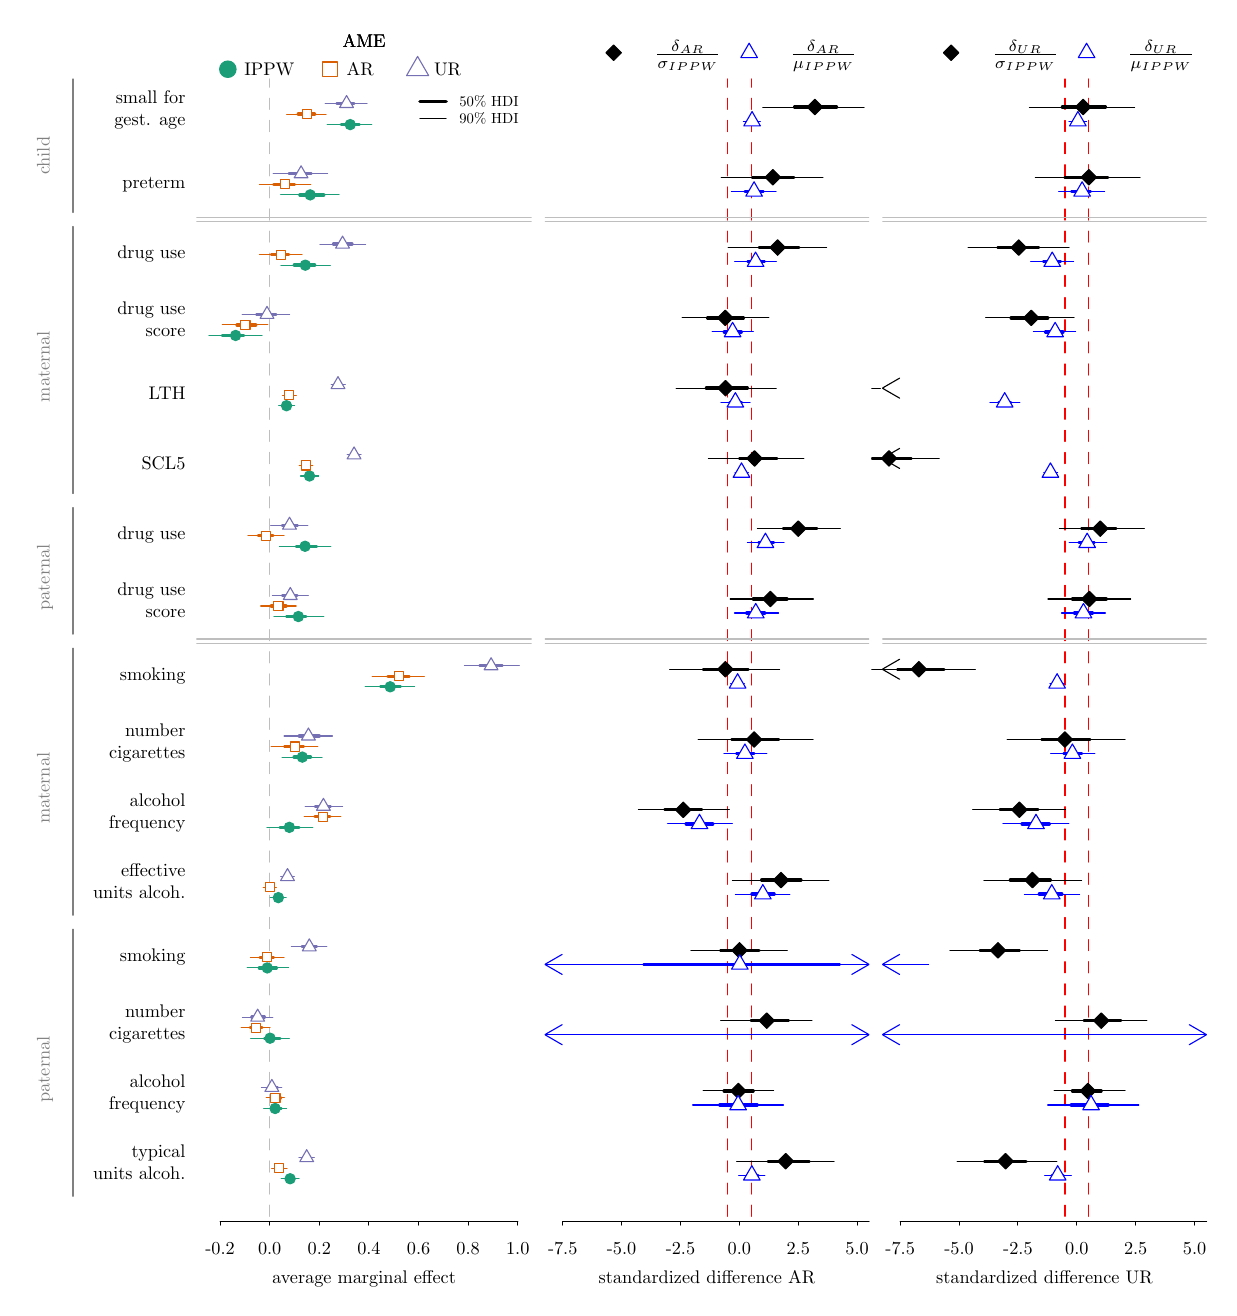
\begin{tikzpicture}[x=1pt,y=1pt]
\definecolor{fillColor}{RGB}{255,255,255}
\path[use as bounding box,fill=fillColor,fill opacity=0.00] (0,0) rectangle (426.79,455.24);
\begin{scope}
\path[clip] (  0.00, 23.76) rectangle ( 60.97,443.36);
\definecolor{drawColor}{RGB}{0,0,0}

\node[text=drawColor,anchor=base east,inner sep=0pt, outer sep=0pt, scale=  0.66] at ( 57.01,427.78) {small for};

\node[text=drawColor,anchor=base east,inner sep=0pt, outer sep=0pt, scale=  0.66] at ( 57.01,419.86) {gest. age};

\node[text=drawColor,anchor=base east,inner sep=0pt, outer sep=0pt, scale=  0.66] at ( 57.01,397.11) {preterm};

\node[text=drawColor,anchor=base east,inner sep=0pt, outer sep=0pt, scale=  0.66] at ( 57.01,371.71) {drug use};

\node[text=drawColor,anchor=base east,inner sep=0pt, outer sep=0pt, scale=  0.66] at ( 57.01,351.60) {drug use};

\node[text=drawColor,anchor=base east,inner sep=0pt, outer sep=0pt, scale=  0.66] at ( 57.01,343.68) {score};

\node[text=drawColor,anchor=base east,inner sep=0pt, outer sep=0pt, scale=  0.66] at ( 57.01,320.92) {LTH};

\node[text=drawColor,anchor=base east,inner sep=0pt, outer sep=0pt, scale=  0.66] at ( 57.01,295.53) {SCL5};

\node[text=drawColor,anchor=base east,inner sep=0pt, outer sep=0pt, scale=  0.66] at ( 57.01,270.14) {drug use};

\node[text=drawColor,anchor=base east,inner sep=0pt, outer sep=0pt, scale=  0.66] at ( 57.01,250.02) {drug use};

\node[text=drawColor,anchor=base east,inner sep=0pt, outer sep=0pt, scale=  0.66] at ( 57.01,242.10) {score};

\node[text=drawColor,anchor=base east,inner sep=0pt, outer sep=0pt, scale=  0.66] at ( 57.01,219.35) {smoking};

\node[text=drawColor,anchor=base east,inner sep=0pt, outer sep=0pt, scale=  0.66] at ( 57.01,199.24) {number};

\node[text=drawColor,anchor=base east,inner sep=0pt, outer sep=0pt, scale=  0.66] at ( 57.01,191.32) {cigarettes};

\node[text=drawColor,anchor=base east,inner sep=0pt, outer sep=0pt, scale=  0.66] at ( 57.01,173.84) {alcohol };

\node[text=drawColor,anchor=base east,inner sep=0pt, outer sep=0pt, scale=  0.66] at ( 57.01,165.92) {frequency};

\node[text=drawColor,anchor=base east,inner sep=0pt, outer sep=0pt, scale=  0.66] at ( 57.01,148.45) {effective};

\node[text=drawColor,anchor=base east,inner sep=0pt, outer sep=0pt, scale=  0.66] at ( 57.01,140.53) {units alcoh.};

\node[text=drawColor,anchor=base east,inner sep=0pt, outer sep=0pt, scale=  0.66] at ( 57.01,117.78) {smoking};

\node[text=drawColor,anchor=base east,inner sep=0pt, outer sep=0pt, scale=  0.66] at ( 57.01, 97.66) {number};

\node[text=drawColor,anchor=base east,inner sep=0pt, outer sep=0pt, scale=  0.66] at ( 57.01, 89.74) {cigarettes};

\node[text=drawColor,anchor=base east,inner sep=0pt, outer sep=0pt, scale=  0.66] at ( 57.01, 72.27) {alcohol };

\node[text=drawColor,anchor=base east,inner sep=0pt, outer sep=0pt, scale=  0.66] at ( 57.01, 64.35) {frequency};

\node[text=drawColor,anchor=base east,inner sep=0pt, outer sep=0pt, scale=  0.66] at ( 57.01, 46.88) {typical};

\node[text=drawColor,anchor=base east,inner sep=0pt, outer sep=0pt, scale=  0.66] at ( 57.01, 38.96) {units alcoh.};
\definecolor{drawColor}{gray}{0.50}

\path[draw=drawColor,line width= 0.4pt,line join=round,line cap=round] ( 16.37,436.71) -- ( 16.37,388.46);

\path[draw=drawColor,line width= 0.4pt,line join=round,line cap=round] ( 16.37,383.38) -- ( 16.37,286.89);

\path[draw=drawColor,line width= 0.4pt,line join=round,line cap=round] ( 16.37,281.81) -- ( 16.37,236.10);

\path[draw=drawColor,line width= 0.4pt,line join=round,line cap=round] ( 16.37,231.02) -- ( 16.37,134.53);

\path[draw=drawColor,line width= 0.4pt,line join=round,line cap=round] ( 16.37,129.45) -- ( 16.37, 32.95);

\node[text=drawColor,rotate= 90.00,anchor=base,inner sep=0pt, outer sep=0pt, scale=  0.66] at (  7.90,408.93) {child};

\node[text=drawColor,rotate= 90.00,anchor=base,inner sep=0pt, outer sep=0pt, scale=  0.66] at (  7.90,332.75) {maternal};

\node[text=drawColor,rotate= 90.00,anchor=base,inner sep=0pt, outer sep=0pt, scale=  0.66] at (  7.90,256.57) {paternal};

\node[text=drawColor,rotate= 90.00,anchor=base,inner sep=0pt, outer sep=0pt, scale=  0.66] at (  7.90,180.39) {maternal};

\node[text=drawColor,rotate= 90.00,anchor=base,inner sep=0pt, outer sep=0pt, scale=  0.66] at (  7.90, 78.81) {paternal};
\end{scope}
\begin{scope}
\path[clip] (  0.00,  0.00) rectangle (426.79,455.24);
\definecolor{drawColor}{RGB}{0,0,0}

\path[draw=drawColor,line width= 0.4pt,line join=round,line cap=round] ( 69.54, 23.76) -- (177.09, 23.76);

\path[draw=drawColor,line width= 0.4pt,line join=round,line cap=round] ( 69.54, 23.76) -- ( 69.54, 22.55);

\path[draw=drawColor,line width= 0.4pt,line join=round,line cap=round] ( 87.46, 23.76) -- ( 87.46, 22.55);

\path[draw=drawColor,line width= 0.4pt,line join=round,line cap=round] (105.39, 23.76) -- (105.39, 22.55);

\path[draw=drawColor,line width= 0.4pt,line join=round,line cap=round] (123.31, 23.76) -- (123.31, 22.55);

\path[draw=drawColor,line width= 0.4pt,line join=round,line cap=round] (141.24, 23.76) -- (141.24, 22.55);

\path[draw=drawColor,line width= 0.4pt,line join=round,line cap=round] (159.16, 23.76) -- (159.16, 22.55);

\path[draw=drawColor,line width= 0.4pt,line join=round,line cap=round] (177.09, 23.76) -- (177.09, 22.55);

\node[text=drawColor,anchor=base,inner sep=0pt, outer sep=0pt, scale=  0.66] at ( 69.54, 11.88) {-0.2};

\node[text=drawColor,anchor=base,inner sep=0pt, outer sep=0pt, scale=  0.66] at ( 87.46, 11.88) {0.0};

\node[text=drawColor,anchor=base,inner sep=0pt, outer sep=0pt, scale=  0.66] at (105.39, 11.88) {0.2};

\node[text=drawColor,anchor=base,inner sep=0pt, outer sep=0pt, scale=  0.66] at (123.31, 11.88) {0.4};

\node[text=drawColor,anchor=base,inner sep=0pt, outer sep=0pt, scale=  0.66] at (141.24, 11.88) {0.6};

\node[text=drawColor,anchor=base,inner sep=0pt, outer sep=0pt, scale=  0.66] at (159.16, 11.88) {0.8};

\node[text=drawColor,anchor=base,inner sep=0pt, outer sep=0pt, scale=  0.66] at (177.09, 11.88) {1.0};
\end{scope}
\begin{scope}
\path[clip] ( 60.97,  0.00) rectangle (182.91,455.24);
\definecolor{drawColor}{RGB}{0,0,0}

\node[text=drawColor,anchor=base,inner sep=0pt, outer sep=0pt, scale=  0.66] at (121.54,  1.58) {average marginal effect};
\end{scope}
\begin{scope}
\path[clip] ( 60.97, 23.76) rectangle (182.12,443.36);
\definecolor{drawColor}{RGB}{190,190,190}

\path[draw=drawColor,line width= 0.4pt,dash pattern=on 4pt off 4pt ,line join=round,line cap=round] ( 87.46, 17.72) --
	( 87.46,436.71);
\definecolor{drawColor}{RGB}{27,158,119}

\path[draw=drawColor,line width= 1.2pt,line join=round,line cap=round] (113.25,420.21) -- (119.87,420.21);

\path[draw=drawColor,line width= 1.2pt,line join=round,line cap=round] ( 98.36,394.81) -- (106.99,394.81);

\path[draw=drawColor,line width= 1.2pt,line join=round,line cap=round] ( 96.34,369.42) -- (103.69,369.42);

\path[draw=drawColor,line width= 1.2pt,line join=round,line cap=round] ( 70.30,344.02) -- ( 78.08,344.02);

\path[draw=drawColor,line width= 1.2pt,line join=round,line cap=round] ( 92.31,318.63) -- ( 94.68,318.63);

\path[draw=drawColor,line width= 1.2pt,line join=round,line cap=round] (100.56,293.24) -- (103.17,293.24);

\path[draw=drawColor,line width= 1.2pt,line join=round,line cap=round] ( 97.04,267.84) -- (104.43,267.84);

\path[draw=drawColor,line width= 1.2pt,line join=round,line cap=round] ( 93.53,242.45) -- (100.56,242.45);

\path[draw=drawColor,line width= 1.2pt,line join=round,line cap=round] (127.45,217.06) -- (134.74,217.06);

\path[draw=drawColor,line width= 1.2pt,line join=round,line cap=round] ( 96.29,191.66) -- (102.19,191.66);

\path[draw=drawColor,line width= 1.2pt,line join=round,line cap=round] ( 91.16,166.27) -- ( 98.06,166.27);

\path[draw=drawColor,line width= 1.2pt,line join=round,line cap=round] ( 89.56,140.88) -- ( 91.88,140.88);

\path[draw=drawColor,line width= 1.2pt,line join=round,line cap=round] ( 83.73,115.48) -- ( 89.86,115.48);

\path[draw=drawColor,line width= 1.2pt,line join=round,line cap=round] ( 85.52, 90.09) -- ( 91.23, 90.09);

\path[draw=drawColor,line width= 1.2pt,line join=round,line cap=round] ( 88.51, 64.69) -- ( 91.66, 64.69);

\path[draw=drawColor,line width= 1.2pt,line join=round,line cap=round] ( 93.56, 39.30) -- ( 96.27, 39.30);

\path[draw=drawColor,line width= 0.4pt,line join=round,line cap=round] (108.23,420.21) -- (124.32,420.21);

\path[draw=drawColor,line width= 0.4pt,line join=round,line cap=round] ( 91.37,394.81) -- (112.53,394.81);

\path[draw=drawColor,line width= 0.4pt,line join=round,line cap=round] ( 91.47,369.42) -- (109.35,369.42);

\path[draw=drawColor,line width= 0.4pt,line join=round,line cap=round] ( 65.46,344.02) -- ( 84.74,344.02);

\path[draw=drawColor,line width= 0.4pt,line join=round,line cap=round] ( 90.67,318.63) -- ( 96.46,318.63);

\path[draw=drawColor,line width= 0.4pt,line join=round,line cap=round] ( 98.62,293.24) -- (105.16,293.24);

\path[draw=drawColor,line width= 0.4pt,line join=round,line cap=round] ( 90.95,267.84) -- (109.57,267.84);

\path[draw=drawColor,line width= 0.4pt,line join=round,line cap=round] ( 88.97,242.45) -- (107.05,242.45);

\path[draw=drawColor,line width= 0.4pt,line join=round,line cap=round] (121.97,217.06) -- (139.83,217.06);

\path[draw=drawColor,line width= 0.4pt,line join=round,line cap=round] ( 91.91,191.66) -- (106.35,191.66);

\path[draw=drawColor,line width= 0.4pt,line join=round,line cap=round] ( 86.47,166.27) -- (103.02,166.27);

\path[draw=drawColor,line width= 0.4pt,line join=round,line cap=round] ( 87.62,140.88) -- ( 93.42,140.88);

\path[draw=drawColor,line width= 0.4pt,line join=round,line cap=round] ( 79.28,115.48) -- ( 94.27,115.48);

\path[draw=drawColor,line width= 0.4pt,line join=round,line cap=round] ( 80.58, 90.09) -- ( 94.57, 90.09);

\path[draw=drawColor,line width= 0.4pt,line join=round,line cap=round] ( 85.31, 64.69) -- ( 93.56, 64.69);

\path[draw=drawColor,line width= 0.4pt,line join=round,line cap=round] ( 91.58, 39.30) -- ( 98.07, 39.30);
\definecolor{fillColor}{RGB}{27,158,119}

\path[draw=drawColor,line width= 0.4pt,line join=round,line cap=round,fill=fillColor] (116.55,420.21) circle (  1.86);

\path[draw=drawColor,line width= 0.4pt,line join=round,line cap=round,fill=fillColor] (102.09,394.81) circle (  1.86);

\path[draw=drawColor,line width= 0.4pt,line join=round,line cap=round,fill=fillColor] (100.33,369.42) circle (  1.86);

\path[draw=drawColor,line width= 0.4pt,line join=round,line cap=round,fill=fillColor] ( 75.13,344.02) circle (  1.86);

\path[draw=drawColor,line width= 0.4pt,line join=round,line cap=round,fill=fillColor] ( 93.53,318.63) circle (  1.86);

\path[draw=drawColor,line width= 0.4pt,line join=round,line cap=round,fill=fillColor] (101.84,293.24) circle (  1.86);

\path[draw=drawColor,line width= 0.4pt,line join=round,line cap=round,fill=fillColor] (100.23,267.84) circle (  1.86);

\path[draw=drawColor,line width= 0.4pt,line join=round,line cap=round,fill=fillColor] ( 97.81,242.45) circle (  1.86);

\path[draw=drawColor,line width= 0.4pt,line join=round,line cap=round,fill=fillColor] (131.00,217.06) circle (  1.86);

\path[draw=drawColor,line width= 0.4pt,line join=round,line cap=round,fill=fillColor] ( 99.24,191.66) circle (  1.86);

\path[draw=drawColor,line width= 0.4pt,line join=round,line cap=round,fill=fillColor] ( 94.56,166.27) circle (  1.86);

\path[draw=drawColor,line width= 0.4pt,line join=round,line cap=round,fill=fillColor] ( 90.58,140.88) circle (  1.86);

\path[draw=drawColor,line width= 0.4pt,line join=round,line cap=round,fill=fillColor] ( 86.56,115.48) circle (  1.86);

\path[draw=drawColor,line width= 0.4pt,line join=round,line cap=round,fill=fillColor] ( 87.58, 90.09) circle (  1.86);

\path[draw=drawColor,line width= 0.4pt,line join=round,line cap=round,fill=fillColor] ( 89.42, 64.69) circle (  1.86);

\path[draw=drawColor,line width= 0.4pt,line join=round,line cap=round,fill=fillColor] ( 94.83, 39.30) circle (  1.86);
\definecolor{drawColor}{RGB}{217,95,2}

\path[draw=drawColor,line width= 1.2pt,line join=round,line cap=round] ( 97.80,424.01) -- (103.66,424.01);

\path[draw=drawColor,line width= 1.2pt,line join=round,line cap=round] ( 88.85,398.62) -- ( 96.48,398.62);

\path[draw=drawColor,line width= 1.2pt,line join=round,line cap=round] ( 88.03,373.23) -- ( 94.37,373.23);

\path[draw=drawColor,line width= 1.2pt,line join=round,line cap=round] ( 75.66,347.83) -- ( 82.42,347.83);

\path[draw=drawColor,line width= 1.2pt,line join=round,line cap=round] ( 93.54,322.44) -- ( 95.57,322.44);

\path[draw=drawColor,line width= 1.2pt,line join=round,line cap=round] ( 99.58,297.05) -- (101.61,297.05);

\path[draw=drawColor,line width= 1.2pt,line join=round,line cap=round] ( 83.29,271.65) -- ( 88.68,271.65);

\path[draw=drawColor,line width= 1.2pt,line join=round,line cap=round] ( 88.02,246.26) -- ( 93.33,246.26);

\path[draw=drawColor,line width= 1.2pt,line join=round,line cap=round] (130.13,220.87) -- (137.91,220.87);

\path[draw=drawColor,line width= 1.2pt,line join=round,line cap=round] ( 92.80,195.47) -- ( 99.73,195.47);

\path[draw=drawColor,line width= 1.2pt,line join=round,line cap=round] (103.75,170.08) -- (109.23,170.08);

\path[draw=drawColor,line width= 1.2pt,line join=round,line cap=round] ( 86.49,144.68) -- ( 88.45,144.68);

\path[draw=drawColor,line width= 1.2pt,line join=round,line cap=round] ( 83.92,119.29) -- ( 88.89,119.29);

\path[draw=drawColor,line width= 1.2pt,line join=round,line cap=round] ( 80.41, 93.90) -- ( 84.72, 93.90);

\path[draw=drawColor,line width= 1.2pt,line join=round,line cap=round] ( 88.76, 68.50) -- ( 91.30, 68.50);

\path[draw=drawColor,line width= 1.2pt,line join=round,line cap=round] ( 89.71, 43.11) -- ( 91.99, 43.11);

\path[draw=drawColor,line width= 0.4pt,line join=round,line cap=round] ( 93.55,424.01) -- (107.81,424.01);

\path[draw=drawColor,line width= 0.4pt,line join=round,line cap=round] ( 83.70,398.62) -- (102.28,398.62);

\path[draw=drawColor,line width= 0.4pt,line join=round,line cap=round] ( 83.70,373.23) -- ( 99.19,373.23);

\path[draw=drawColor,line width= 0.4pt,line join=round,line cap=round] ( 70.32,347.83) -- ( 86.81,347.83);

\path[draw=drawColor,line width= 0.4pt,line join=round,line cap=round] ( 92.09,322.44) -- ( 97.05,322.44);

\path[draw=drawColor,line width= 0.4pt,line join=round,line cap=round] ( 98.09,297.05) -- (103.07,297.05);

\path[draw=drawColor,line width= 0.4pt,line join=round,line cap=round] ( 79.60,271.65) -- ( 92.66,271.65);

\path[draw=drawColor,line width= 0.4pt,line join=round,line cap=round] ( 84.20,246.26) -- ( 97.02,246.26);

\path[draw=drawColor,line width= 0.4pt,line join=round,line cap=round] (124.49,220.87) -- (143.37,220.87);

\path[draw=drawColor,line width= 0.4pt,line join=round,line cap=round] ( 87.96,195.47) -- (104.86,195.47);

\path[draw=drawColor,line width= 0.4pt,line join=round,line cap=round] ( 99.93,170.08) -- (113.13,170.08);

\path[draw=drawColor,line width= 0.4pt,line join=round,line cap=round] ( 85.08,144.68) -- ( 89.87,144.68);

\path[draw=drawColor,line width= 0.4pt,line join=round,line cap=round] ( 80.51,119.29) -- ( 92.64,119.29);

\path[draw=drawColor,line width= 0.4pt,line join=round,line cap=round] ( 77.11, 93.90) -- ( 87.56, 93.90);

\path[draw=drawColor,line width= 0.4pt,line join=round,line cap=round] ( 86.14, 68.50) -- ( 92.79, 68.50);

\path[draw=drawColor,line width= 0.4pt,line join=round,line cap=round] ( 88.17, 43.11) -- ( 93.71, 43.11);
\definecolor{fillColor}{RGB}{255,255,255}

\path[draw=drawColor,line width= 0.4pt,line join=round,line cap=round,fill=fillColor] ( 99.20,422.37) rectangle (102.49,425.66);

\path[draw=drawColor,line width= 0.4pt,line join=round,line cap=round,fill=fillColor] ( 91.31,396.98) rectangle ( 94.60,400.27);

\path[draw=drawColor,line width= 0.4pt,line join=round,line cap=round,fill=fillColor] ( 89.83,371.58) rectangle ( 93.12,374.87);

\path[draw=drawColor,line width= 0.4pt,line join=round,line cap=round,fill=fillColor] ( 77.03,346.19) rectangle ( 80.32,349.48);

\path[draw=drawColor,line width= 0.4pt,line join=round,line cap=round,fill=fillColor] ( 92.92,320.79) rectangle ( 96.21,324.08);

\path[draw=drawColor,line width= 0.4pt,line join=round,line cap=round,fill=fillColor] ( 98.89,295.40) rectangle (102.18,298.69);

\path[draw=drawColor,line width= 0.4pt,line join=round,line cap=round,fill=fillColor] ( 84.45,270.01) rectangle ( 87.74,273.30);

\path[draw=drawColor,line width= 0.4pt,line join=round,line cap=round,fill=fillColor] ( 88.96,244.61) rectangle ( 92.25,247.90);

\path[draw=drawColor,line width= 0.4pt,line join=round,line cap=round,fill=fillColor] (132.60,219.22) rectangle (135.89,222.51);

\path[draw=drawColor,line width= 0.4pt,line join=round,line cap=round,fill=fillColor] ( 94.82,193.83) rectangle ( 98.11,197.12);

\path[draw=drawColor,line width= 0.4pt,line join=round,line cap=round,fill=fillColor] (104.94,168.43) rectangle (108.23,171.72);

\path[draw=drawColor,line width= 0.4pt,line join=round,line cap=round,fill=fillColor] ( 85.83,143.04) rectangle ( 89.12,146.33);

\path[draw=drawColor,line width= 0.4pt,line join=round,line cap=round,fill=fillColor] ( 84.90,117.65) rectangle ( 88.19,120.94);

\path[draw=drawColor,line width= 0.4pt,line join=round,line cap=round,fill=fillColor] ( 80.89, 92.25) rectangle ( 84.18, 95.54);

\path[draw=drawColor,line width= 0.4pt,line join=round,line cap=round,fill=fillColor] ( 87.88, 66.86) rectangle ( 91.17, 70.15);

\path[draw=drawColor,line width= 0.4pt,line join=round,line cap=round,fill=fillColor] ( 89.29, 41.46) rectangle ( 92.58, 44.75);
\definecolor{drawColor}{RGB}{117,112,179}

\path[draw=drawColor,line width= 1.2pt,line join=round,line cap=round] (111.69,427.82) -- (117.95,427.82);

\path[draw=drawColor,line width= 1.2pt,line join=round,line cap=round] ( 94.41,402.43) -- (102.47,402.43);

\path[draw=drawColor,line width= 1.2pt,line join=round,line cap=round] (110.52,377.04) -- (117.19,377.04);

\path[draw=drawColor,line width= 1.2pt,line join=round,line cap=round] ( 82.68,351.64) -- ( 89.75,351.64);

\path[draw=drawColor,line width= 1.2pt,line join=round,line cap=round] (111.15,326.25) -- (113.24,326.25);

\path[draw=drawColor,line width= 1.2pt,line join=round,line cap=round] (116.97,300.86) -- (119.05,300.86);

\path[draw=drawColor,line width= 1.2pt,line join=round,line cap=round] ( 91.97,275.46) -- ( 97.55,275.46);

\path[draw=drawColor,line width= 1.2pt,line join=round,line cap=round] ( 92.01,250.07) -- ( 97.39,250.07);

\path[draw=drawColor,line width= 1.2pt,line join=round,line cap=round] (163.36,224.67) -- (171.49,224.67);

\path[draw=drawColor,line width= 1.2pt,line join=round,line cap=round] ( 98.13,199.28) -- (105.37,199.28);

\path[draw=drawColor,line width= 1.2pt,line join=round,line cap=round] (103.90,173.89) -- (109.47,173.89);

\path[draw=drawColor,line width= 1.2pt,line join=round,line cap=round] ( 92.79,148.49) -- ( 94.85,148.49);

\path[draw=drawColor,line width= 1.2pt,line join=round,line cap=round] ( 99.11,123.10) -- (104.43,123.10);

\path[draw=drawColor,line width= 1.2pt,line join=round,line cap=round] ( 81.01, 97.71) -- ( 85.52, 97.71);

\path[draw=drawColor,line width= 1.2pt,line join=round,line cap=round] ( 87.49, 72.31) -- ( 90.29, 72.31);

\path[draw=drawColor,line width= 1.2pt,line join=round,line cap=round] ( 99.68, 46.92) -- (101.95, 46.92);

\path[draw=drawColor,line width= 0.4pt,line join=round,line cap=round] (107.47,427.82) -- (122.65,427.82);

\path[draw=drawColor,line width= 0.4pt,line join=round,line cap=round] ( 88.70,402.43) -- (108.41,402.43);

\path[draw=drawColor,line width= 0.4pt,line join=round,line cap=round] (105.60,377.04) -- (122.14,377.04);

\path[draw=drawColor,line width= 0.4pt,line join=round,line cap=round] ( 77.50,351.64) -- ( 94.63,351.64);

\path[draw=drawColor,line width= 0.4pt,line join=round,line cap=round] (109.63,326.25) -- (114.77,326.25);

\path[draw=drawColor,line width= 0.4pt,line join=round,line cap=round] (115.42,300.86) -- (120.49,300.86);

\path[draw=drawColor,line width= 0.4pt,line join=round,line cap=round] ( 87.77,275.46) -- (101.25,275.46);

\path[draw=drawColor,line width= 0.4pt,line join=round,line cap=round] ( 88.44,250.07) -- (101.39,250.07);

\path[draw=drawColor,line width= 0.4pt,line join=round,line cap=round] (157.80,224.67) -- (177.63,224.67);

\path[draw=drawColor,line width= 0.4pt,line join=round,line cap=round] ( 92.67,199.28) -- (110.12,199.28);

\path[draw=drawColor,line width= 0.4pt,line join=round,line cap=round] (100.24,173.89) -- (113.82,173.89);

\path[draw=drawColor,line width= 0.4pt,line join=round,line cap=round] ( 91.41,148.49) -- ( 96.38,148.49);

\path[draw=drawColor,line width= 0.4pt,line join=round,line cap=round] ( 95.26,123.10) -- (108.11,123.10);

\path[draw=drawColor,line width= 0.4pt,line join=round,line cap=round] ( 77.60, 97.71) -- ( 88.58, 97.71);

\path[draw=drawColor,line width= 0.4pt,line join=round,line cap=round] ( 84.48, 72.31) -- ( 91.80, 72.31);

\path[draw=drawColor,line width= 0.4pt,line join=round,line cap=round] ( 98.02, 46.92) -- (103.59, 46.92);

\path[draw=drawColor,line width= 0.4pt,line join=round,line cap=round,fill=fillColor] (115.23,430.71) --
	(117.73,426.38) --
	(112.73,426.38) --
	cycle;

\path[draw=drawColor,line width= 0.4pt,line join=round,line cap=round,fill=fillColor] ( 98.80,405.32) --
	(101.30,400.99) --
	( 96.30,400.99) --
	cycle;

\path[draw=drawColor,line width= 0.4pt,line join=round,line cap=round,fill=fillColor] (113.78,379.92) --
	(116.28,375.59) --
	(111.28,375.59) --
	cycle;

\path[draw=drawColor,line width= 0.4pt,line join=round,line cap=round,fill=fillColor] ( 86.48,354.53) --
	( 88.98,350.20) --
	( 83.98,350.20) --
	cycle;

\path[draw=drawColor,line width= 0.4pt,line join=round,line cap=round,fill=fillColor] (112.13,329.14) --
	(114.63,324.81) --
	(109.63,324.81) --
	cycle;

\path[draw=drawColor,line width= 0.4pt,line join=round,line cap=round,fill=fillColor] (117.94,303.74) --
	(120.44,299.41) --
	(115.44,299.41) --
	cycle;

\path[draw=drawColor,line width= 0.4pt,line join=round,line cap=round,fill=fillColor] ( 94.61,278.35) --
	( 97.11,274.02) --
	( 92.11,274.02) --
	cycle;

\path[draw=drawColor,line width= 0.4pt,line join=round,line cap=round,fill=fillColor] ( 94.89,252.95) --
	( 97.39,248.62) --
	( 92.39,248.62) --
	cycle;

\path[draw=drawColor,line width= 0.4pt,line join=round,line cap=round,fill=fillColor] (167.45,227.56) --
	(169.95,223.23) --
	(164.95,223.23) --
	cycle;

\path[draw=drawColor,line width= 0.4pt,line join=round,line cap=round,fill=fillColor] (101.45,202.17) --
	(103.95,197.84) --
	( 98.95,197.84) --
	cycle;

\path[draw=drawColor,line width= 0.4pt,line join=round,line cap=round,fill=fillColor] (106.86,176.77) --
	(109.36,172.44) --
	(104.36,172.44) --
	cycle;

\path[draw=drawColor,line width= 0.4pt,line join=round,line cap=round,fill=fillColor] ( 93.89,151.38) --
	( 96.39,147.05) --
	( 91.39,147.05) --
	cycle;

\path[draw=drawColor,line width= 0.4pt,line join=round,line cap=round,fill=fillColor] (101.77,125.99) --
	(104.27,121.66) --
	( 99.27,121.66) --
	cycle;

\path[draw=drawColor,line width= 0.4pt,line join=round,line cap=round,fill=fillColor] ( 83.10,100.59) --
	( 85.60, 96.26) --
	( 80.60, 96.26) --
	cycle;

\path[draw=drawColor,line width= 0.4pt,line join=round,line cap=round,fill=fillColor] ( 88.24, 75.20) --
	( 90.74, 70.87) --
	( 85.74, 70.87) --
	cycle;

\path[draw=drawColor,line width= 0.4pt,line join=round,line cap=round,fill=fillColor] (100.82, 49.81) --
	(103.32, 45.48) --
	( 98.32, 45.48) --
	cycle;
\end{scope}
\begin{scope}
\path[clip] ( 60.97,  0.00) rectangle (182.91,455.24);
\definecolor{drawColor}{RGB}{27,158,119}
\definecolor{fillColor}{RGB}{27,158,119}

\path[draw=drawColor,line width= 0.4pt,line join=round,line cap=round,fill=fillColor] ( 72.33,440.22) circle (  2.97);
\definecolor{drawColor}{RGB}{217,95,2}
\definecolor{fillColor}{RGB}{255,255,255}

\path[draw=drawColor,line width= 0.4pt,line join=round,line cap=round,fill=fillColor] (106.67,437.59) rectangle (111.94,442.85);
\definecolor{drawColor}{RGB}{117,112,179}

\path[draw=drawColor,line width= 0.4pt,line join=round,line cap=round,fill=fillColor] (140.90,444.84) --
	(144.90,437.91) --
	(136.90,437.91) --
	cycle;
\definecolor{drawColor}{RGB}{0,0,0}

\node[text=drawColor,anchor=base,inner sep=0pt, outer sep=0pt, scale=  0.66] at (121.54,448.14) {AME};

\node[text=drawColor,anchor=base,inner sep=0pt, outer sep=0pt, scale=  0.66] at (121.54,448.14) {AME};

\node[text=drawColor,anchor=base,inner sep=0pt, outer sep=0pt, scale=  0.66] at (121.54,448.14) {AME};

\node[text=drawColor,anchor=base west,inner sep=0pt, outer sep=0pt, scale=  0.66] at ( 78.27,437.95) {IPPW};

\node[text=drawColor,anchor=base west,inner sep=0pt, outer sep=0pt, scale=  0.66] at (115.24,437.95) {AR};

\node[text=drawColor,anchor=base west,inner sep=0pt, outer sep=0pt, scale=  0.66] at (146.84,437.95) {UR};
\end{scope}
\begin{scope}
\path[clip] ( 60.97, 23.76) rectangle (182.12,443.36);
\definecolor{drawColor}{RGB}{0,0,0}

\path[draw=drawColor,line width= 1.2pt,line join=round,line cap=round] (141.73,428.64) -- (151.23,428.64);

\path[draw=drawColor,line width= 0.4pt,line join=round,line cap=round] (141.73,422.30) -- (151.23,422.30);

\node[text=drawColor,anchor=base west,inner sep=0pt, outer sep=0pt, scale=  0.53] at (155.98,426.82) {50\% HDI};

\node[text=drawColor,anchor=base west,inner sep=0pt, outer sep=0pt, scale=  0.53] at (155.98,420.48) {90\% HDI};
\definecolor{drawColor}{RGB}{190,190,190}

\path[draw=drawColor,line width= 0.4pt,line join=round,line cap=round] ( 60.97,385.16) -- (182.12,385.16);

\path[draw=drawColor,line width= 0.4pt,line join=round,line cap=round] ( 60.97,386.69) -- (182.12,386.69);

\path[draw=drawColor,line width= 0.4pt,line join=round,line cap=round] ( 60.97,232.80) -- (182.12,232.80);

\path[draw=drawColor,line width= 0.4pt,line join=round,line cap=round] ( 60.97,234.32) -- (182.12,234.32);
\end{scope}
\begin{scope}
\path[clip] (182.91,  0.00) rectangle (304.85,455.24);
\definecolor{drawColor}{RGB}{0,0,0}

\node[text=drawColor,anchor=base,inner sep=0pt, outer sep=0pt, scale=  0.66] at (245.46,  1.58) {standardized difference AR};
\end{scope}
\begin{scope}
\path[clip] (  0.00,  0.00) rectangle (426.79,455.24);
\definecolor{drawColor}{RGB}{0,0,0}

\path[draw=drawColor,line width= 0.4pt,line join=round,line cap=round] (193.34, 23.76) -- (304.06, 23.76);

\path[draw=drawColor,line width= 0.4pt,line join=round,line cap=round] (193.34, 23.76) -- (193.34, 22.59);

\path[draw=drawColor,line width= 0.4pt,line join=round,line cap=round] (214.61, 23.76) -- (214.61, 22.59);

\path[draw=drawColor,line width= 0.4pt,line join=round,line cap=round] (235.89, 23.76) -- (235.89, 22.59);

\path[draw=drawColor,line width= 0.4pt,line join=round,line cap=round] (257.17, 23.76) -- (257.17, 22.59);

\path[draw=drawColor,line width= 0.4pt,line join=round,line cap=round] (278.44, 23.76) -- (278.44, 22.59);

\path[draw=drawColor,line width= 0.4pt,line join=round,line cap=round] (299.72, 23.76) -- (299.72, 22.59);

\node[text=drawColor,anchor=base,inner sep=0pt, outer sep=0pt, scale=  0.66] at (193.34, 11.88) {-7.5};

\node[text=drawColor,anchor=base,inner sep=0pt, outer sep=0pt, scale=  0.66] at (214.61, 11.88) {-5.0};

\node[text=drawColor,anchor=base,inner sep=0pt, outer sep=0pt, scale=  0.66] at (235.89, 11.88) {-2.5};

\node[text=drawColor,anchor=base,inner sep=0pt, outer sep=0pt, scale=  0.66] at (257.17, 11.88) {0.0};

\node[text=drawColor,anchor=base,inner sep=0pt, outer sep=0pt, scale=  0.66] at (278.44, 11.88) {2.5};

\node[text=drawColor,anchor=base,inner sep=0pt, outer sep=0pt, scale=  0.66] at (299.72, 11.88) {5.0};
\end{scope}
\begin{scope}
\path[clip] (186.87, 23.76) rectangle (304.06,443.36);
\definecolor{drawColor}{RGB}{255,0,0}

\path[draw=drawColor,line width= 0.4pt,dash pattern=on 4pt off 4pt ,line join=round,line cap=round] (252.91, 17.72) -- (252.91,436.71);

\path[draw=drawColor,line width= 0.4pt,dash pattern=on 4pt off 4pt ,line join=round,line cap=round] (261.42, 17.72) -- (261.42,436.71);
\end{scope}
\begin{scope}
\path[clip] (182.91,  0.00) rectangle (304.85,455.24);
\definecolor{drawColor}{RGB}{0,0,0}

\path[draw=drawColor,line width= 0.4pt,line join=round,line cap=round] (265.63,426.55) -- (302.25,426.55);

\path[draw=drawColor,line width= 0.4pt,line join=round,line cap=round] (250.63,401.16) -- (287.37,401.16);

\path[draw=drawColor,line width= 0.4pt,line join=round,line cap=round] (253.08,375.77) -- (288.68,375.77);

\path[draw=drawColor,line width= 0.4pt,line join=round,line cap=round] (236.49,350.37) -- (267.78,350.37);

\path[draw=drawColor,line width= 0.4pt,line join=round,line cap=round] (234.30,324.98) -- (270.48,324.98);

\path[draw=drawColor,line width= 0.4pt,line join=round,line cap=round] (246.00,299.59) -- (280.47,299.59);

\path[draw=drawColor,line width= 0.4pt,line join=round,line cap=round] (263.67,274.19) -- (293.65,274.19);

\path[draw=drawColor,line width= 0.4pt,line join=round,line cap=round] (253.87,248.80) -- (283.90,248.80);

\path[draw=drawColor,line width= 0.4pt,line join=round,line cap=round] (231.94,223.40) -- (271.73,223.40);

\path[draw=drawColor,line width= 0.4pt,line join=round,line cap=round] (242.31,198.01) -- (283.81,198.01);

\path[draw=drawColor,line width= 0.4pt,line join=round,line cap=round] (220.65,172.62) -- (253.55,172.62);

\path[draw=drawColor,line width= 0.4pt,line join=round,line cap=round] (254.67,147.22) -- (289.46,147.22);

\path[draw=drawColor,line width= 0.4pt,line join=round,line cap=round] (239.69,121.83) -- (274.46,121.83);

\path[draw=drawColor,line width= 0.4pt,line join=round,line cap=round] (250.39, 96.44) -- (283.40, 96.44);

\path[draw=drawColor,line width= 0.4pt,line join=round,line cap=round] (244.05, 71.04) -- (269.54, 71.04);

\path[draw=drawColor,line width= 0.4pt,line join=round,line cap=round] (256.16, 45.65) -- (291.40, 45.65);

\path[draw=drawColor,line width= 1.2pt,line join=round,line cap=round] (277.12,426.55) -- (292.28,426.55);

\path[draw=drawColor,line width= 1.2pt,line join=round,line cap=round] (261.77,401.16) -- (276.89,401.16);

\path[draw=drawColor,line width= 1.2pt,line join=round,line cap=round] (264.28,375.77) -- (278.70,375.77);

\path[draw=drawColor,line width= 1.2pt,line join=round,line cap=round] (245.68,350.37) -- (258.61,350.37);

\path[draw=drawColor,line width= 1.2pt,line join=round,line cap=round] (245.25,324.98) -- (260.05,324.98);

\path[draw=drawColor,line width= 1.2pt,line join=round,line cap=round] (257.16,299.59) -- (270.75,299.59);

\path[draw=drawColor,line width= 1.2pt,line join=round,line cap=round] (273.00,274.19) -- (285.20,274.19);

\path[draw=drawColor,line width= 1.2pt,line join=round,line cap=round] (262.23,248.80) -- (274.39,248.80);

\path[draw=drawColor,line width= 1.2pt,line join=round,line cap=round] (244.11,223.40) -- (260.37,223.40);

\path[draw=drawColor,line width= 1.2pt,line join=round,line cap=round] (254.36,198.01) -- (271.42,198.01);

\path[draw=drawColor,line width= 1.2pt,line join=round,line cap=round] (230.15,172.62) -- (243.61,172.62);

\path[draw=drawColor,line width= 1.2pt,line join=round,line cap=round] (265.23,147.22) -- (279.41,147.22);

\path[draw=drawColor,line width= 1.2pt,line join=round,line cap=round] (250.33,121.83) -- (264.33,121.83);

\path[draw=drawColor,line width= 1.2pt,line join=round,line cap=round] (261.38, 96.44) -- (274.98, 96.44);

\path[draw=drawColor,line width= 1.2pt,line join=round,line cap=round] (251.67, 71.04) -- (262.15, 71.04);

\path[draw=drawColor,line width= 1.2pt,line join=round,line cap=round] (267.53, 45.65) -- (282.44, 45.65);
\end{scope}
\begin{scope}
\path[clip] (186.87, 23.76) rectangle (304.06,443.36);
\definecolor{drawColor}{RGB}{0,0,255}

\path[draw=drawColor,line width= 0.4pt,line join=round,line cap=round] (258.59,421.47) -- (264.76,421.47);

\path[draw=drawColor,line width= 0.4pt,line join=round,line cap=round] (254.30,396.08) -- (270.42,396.08);

\path[draw=drawColor,line width= 0.4pt,line join=round,line cap=round] (255.43,370.69) -- (270.52,370.69);

\path[draw=drawColor,line width= 0.4pt,line join=round,line cap=round] (247.34,345.29) -- (262.22,345.29);

\path[draw=drawColor,line width= 0.4pt,line join=round,line cap=round] (250.53,319.90) -- (261.03,319.90);

\path[draw=drawColor,line width= 0.4pt,line join=round,line cap=round] (255.60,294.51) -- (260.44,294.51);

\path[draw=drawColor,line width= 0.4pt,line join=round,line cap=round] (260.04,269.11) -- (273.32,269.11);

\path[draw=drawColor,line width= 0.4pt,line join=round,line cap=round] (255.42,243.72) -- (271.33,243.72);

\path[draw=drawColor,line width= 0.4pt,line join=round,line cap=round] (254.02,218.33) -- (258.98,218.33);

\path[draw=drawColor,line width= 0.4pt,line join=round,line cap=round] (251.62,192.93) -- (267.12,192.93);

\path[draw=drawColor,line width= 0.4pt,line join=round,line cap=round] (231.21,167.54) -- (254.60,167.54);

\path[draw=drawColor,line width= 0.4pt,line join=round,line cap=round] (255.76,142.15) -- (275.39,142.15);

\path[draw=drawColor,line width= 0.4pt,line join=round,line cap=round] (168.78,116.75) -- (344.60,116.75);

\path[draw=drawColor,line width= 0.4pt,line join=round,line cap=round] ( 17.17, 91.36) -- (426.79, 91.36);

\path[draw=drawColor,line width= 0.4pt,line join=round,line cap=round] (240.29, 65.96) -- (273.08, 65.96);

\path[draw=drawColor,line width= 0.4pt,line join=round,line cap=round] (256.90, 40.57) -- (266.37, 40.57);

\path[draw=drawColor,line width= 1.2pt,line join=round,line cap=round] (260.53,421.47) -- (263.08,421.47);

\path[draw=drawColor,line width= 1.2pt,line join=round,line cap=round] (259.19,396.08) -- (265.83,396.08);

\path[draw=drawColor,line width= 1.2pt,line join=round,line cap=round] (260.18,370.69) -- (266.29,370.69);

\path[draw=drawColor,line width= 1.2pt,line join=round,line cap=round] (251.71,345.29) -- (257.85,345.29);

\path[draw=drawColor,line width= 1.2pt,line join=round,line cap=round] (253.71,319.90) -- (258.00,319.90);

\path[draw=drawColor,line width= 1.2pt,line join=round,line cap=round] (257.17,294.51) -- (259.07,294.51);

\path[draw=drawColor,line width= 1.2pt,line join=round,line cap=round] (264.18,269.11) -- (269.58,269.11);

\path[draw=drawColor,line width= 1.2pt,line join=round,line cap=round] (259.85,243.72) -- (266.29,243.72);

\path[draw=drawColor,line width= 1.2pt,line join=round,line cap=round] (255.54,218.33) -- (257.57,218.33);

\path[draw=drawColor,line width= 1.2pt,line join=round,line cap=round] (256.12,192.93) -- (262.49,192.93);

\path[draw=drawColor,line width= 1.2pt,line join=round,line cap=round] (237.96,167.54) -- (247.53,167.54);

\path[draw=drawColor,line width= 1.2pt,line join=round,line cap=round] (261.72,142.15) -- (269.72,142.15);

\path[draw=drawColor,line width= 1.2pt,line join=round,line cap=round] (222.59,116.75) -- (293.41,116.75);

\path[draw=drawColor,line width= 1.2pt,line join=round,line cap=round] (406.32, 91.36) -- (426.79, 91.36);

\path[draw=drawColor,line width= 1.2pt,line join=round,line cap=round] (250.10, 65.96) -- (263.58, 65.96);

\path[draw=drawColor,line width= 1.2pt,line join=round,line cap=round] (259.95, 40.57) -- (263.96, 40.57);

\path[draw=drawColor,line width= 0.4pt,line join=round,line cap=round] (187.22,116.75) -- (186.87,116.75);

\path[draw=drawColor,line width= 0.4pt,line join=round,line cap=round] (193.13,120.36) --
	(186.87,116.75) --
	(193.13,113.14);

\path[draw=drawColor,line width= 0.4pt,line join=round,line cap=round] (187.22, 91.36) -- (186.87, 91.36);

\path[draw=drawColor,line width= 0.4pt,line join=round,line cap=round] (193.13, 94.97) --
	(186.87, 91.36) --
	(193.13, 87.74);

\path[draw=drawColor,line width= 0.4pt,line join=round,line cap=round] (303.82,116.75) -- (304.06,116.75);

\path[draw=drawColor,line width= 0.4pt,line join=round,line cap=round] (297.80,113.14) --
	(304.06,116.75) --
	(297.80,120.36);

\path[draw=drawColor,line width= 0.4pt,line join=round,line cap=round] (303.82, 91.36) -- (304.06, 91.36);

\path[draw=drawColor,line width= 0.4pt,line join=round,line cap=round] (297.80, 87.74) --
	(304.06, 91.36) --
	(297.80, 94.97);
\definecolor{drawColor}{RGB}{0,0,0}
\definecolor{fillColor}{RGB}{0,0,0}

\path[draw=drawColor,line width= 0.4pt,line join=round,line cap=round,fill=fillColor] (284.46,423.76) --
	(287.25,426.55) --
	(284.46,429.35) --
	(281.67,426.55) --
	cycle;

\path[draw=drawColor,line width= 0.4pt,line join=round,line cap=round,fill=fillColor] (269.27,398.37) --
	(272.07,401.16) --
	(269.27,403.95) --
	(266.48,401.16) --
	cycle;

\path[draw=drawColor,line width= 0.4pt,line join=round,line cap=round,fill=fillColor] (270.99,372.97) --
	(273.78,375.77) --
	(270.99,378.56) --
	(268.20,375.77) --
	cycle;

\path[draw=drawColor,line width= 0.4pt,line join=round,line cap=round,fill=fillColor] (252.03,347.58) --
	(254.82,350.37) --
	(252.03,353.16) --
	(249.24,350.37) --
	cycle;

\path[draw=drawColor,line width= 0.4pt,line join=round,line cap=round,fill=fillColor] (252.18,322.19) --
	(254.97,324.98) --
	(252.18,327.77) --
	(249.39,324.98) --
	cycle;

\path[draw=drawColor,line width= 0.4pt,line join=round,line cap=round,fill=fillColor] (262.66,296.79) --
	(265.45,299.59) --
	(262.66,302.38) --
	(259.87,299.59) --
	cycle;

\path[draw=drawColor,line width= 0.4pt,line join=round,line cap=round,fill=fillColor] (278.45,271.40) --
	(281.24,274.19) --
	(278.45,276.98) --
	(275.65,274.19) --
	cycle;

\path[draw=drawColor,line width= 0.4pt,line join=round,line cap=round,fill=fillColor] (268.35,246.01) --
	(271.14,248.80) --
	(268.35,251.59) --
	(265.55,248.80) --
	cycle;

\path[draw=drawColor,line width= 0.4pt,line join=round,line cap=round,fill=fillColor] (252.09,220.61) --
	(254.88,223.40) --
	(252.09,226.20) --
	(249.30,223.40) --
	cycle;

\path[draw=drawColor,line width= 0.4pt,line join=round,line cap=round,fill=fillColor] (262.52,195.22) --
	(265.31,198.01) --
	(262.52,200.80) --
	(259.72,198.01) --
	cycle;

\path[draw=drawColor,line width= 0.4pt,line join=round,line cap=round,fill=fillColor] (236.89,169.83) --
	(239.68,172.62) --
	(236.89,175.41) --
	(234.10,172.62) --
	cycle;

\path[draw=drawColor,line width= 0.4pt,line join=round,line cap=round,fill=fillColor] (272.20,144.43) --
	(274.99,147.22) --
	(272.20,150.02) --
	(269.41,147.22) --
	cycle;

\path[draw=drawColor,line width= 0.4pt,line join=round,line cap=round,fill=fillColor] (257.20,119.04) --
	(259.99,121.83) --
	(257.20,124.62) --
	(254.41,121.83) --
	cycle;

\path[draw=drawColor,line width= 0.4pt,line join=round,line cap=round,fill=fillColor] (267.07, 93.64) --
	(269.86, 96.44) --
	(267.07, 99.23) --
	(264.28, 96.44) --
	cycle;

\path[draw=drawColor,line width= 0.4pt,line join=round,line cap=round,fill=fillColor] (256.81, 68.25) --
	(259.60, 71.04) --
	(256.81, 73.83) --
	(254.02, 71.04) --
	cycle;

\path[draw=drawColor,line width= 0.4pt,line join=round,line cap=round,fill=fillColor] (273.90, 42.86) --
	(276.69, 45.65) --
	(273.90, 48.44) --
	(271.11, 45.65) --
	cycle;
\definecolor{drawColor}{RGB}{0,0,255}
\definecolor{fillColor}{RGB}{255,255,255}

\path[draw=drawColor,line width= 0.4pt,line join=round,line cap=round,fill=fillColor] (261.76,424.94) --
	(264.76,419.74) --
	(258.76,419.74) --
	cycle;

\path[draw=drawColor,line width= 0.4pt,line join=round,line cap=round,fill=fillColor] (262.48,399.55) --
	(265.48,394.35) --
	(259.48,394.35) --
	cycle;

\path[draw=drawColor,line width= 0.4pt,line join=round,line cap=round,fill=fillColor] (263.02,374.15) --
	(266.02,368.96) --
	(260.02,368.96) --
	cycle;

\path[draw=drawColor,line width= 0.4pt,line join=round,line cap=round,fill=fillColor] (254.72,348.76) --
	(257.72,343.56) --
	(251.72,343.56) --
	cycle;

\path[draw=drawColor,line width= 0.4pt,line join=round,line cap=round,fill=fillColor] (255.72,323.36) --
	(258.72,318.17) --
	(252.72,318.17) --
	cycle;

\path[draw=drawColor,line width= 0.4pt,line join=round,line cap=round,fill=fillColor] (257.94,297.97) --
	(260.94,292.77) --
	(254.94,292.77) --
	cycle;

\path[draw=drawColor,line width= 0.4pt,line join=round,line cap=round,fill=fillColor] (266.59,272.58) --
	(269.59,267.38) --
	(263.59,267.38) --
	cycle;

\path[draw=drawColor,line width= 0.4pt,line join=round,line cap=round,fill=fillColor] (263.09,247.18) --
	(266.09,241.99) --
	(260.09,241.99) --
	cycle;

\path[draw=drawColor,line width= 0.4pt,line join=round,line cap=round,fill=fillColor] (256.53,221.79) --
	(259.53,216.59) --
	(253.53,216.59) --
	cycle;

\path[draw=drawColor,line width= 0.4pt,line join=round,line cap=round,fill=fillColor] (259.17,196.40) --
	(262.17,191.20) --
	(256.17,191.20) --
	cycle;

\path[draw=drawColor,line width= 0.4pt,line join=round,line cap=round,fill=fillColor] (242.75,171.00) --
	(245.75,165.81) --
	(239.75,165.81) --
	cycle;

\path[draw=drawColor,line width= 0.4pt,line join=round,line cap=round,fill=fillColor] (265.65,145.61) --
	(268.65,140.41) --
	(262.65,140.41) --
	cycle;

\path[draw=drawColor,line width= 0.4pt,line join=round,line cap=round,fill=fillColor] (257.33,120.22) --
	(260.33,115.02) --
	(254.33,115.02) --
	cycle;

\path[draw=drawColor,line width= 0.4pt,line join=round,line cap=round,fill=fillColor] (256.71, 69.43) --
	(259.71, 64.23) --
	(253.71, 64.23) --
	cycle;

\path[draw=drawColor,line width= 0.4pt,line join=round,line cap=round,fill=fillColor] (261.67, 44.03) --
	(264.67, 38.84) --
	(258.67, 38.84) --
	cycle;
\definecolor{drawColor}{RGB}{190,190,190}

\path[draw=drawColor,line width= 0.4pt,line join=round,line cap=round] (186.87,385.16) -- (304.06,385.16);

\path[draw=drawColor,line width= 0.4pt,line join=round,line cap=round] (186.87,386.69) -- (304.06,386.69);

\path[draw=drawColor,line width= 0.4pt,line join=round,line cap=round] (186.87,232.80) -- (304.06,232.80);

\path[draw=drawColor,line width= 0.4pt,line join=round,line cap=round] (186.87,234.32) -- (304.06,234.32);
\end{scope}
\begin{scope}
\path[clip] (182.91,  0.00) rectangle (304.85,455.24);
\definecolor{drawColor}{RGB}{0,0,0}
\definecolor{fillColor}{RGB}{0,0,0}

\path[draw=drawColor,line width= 0.4pt,line join=round,line cap=round,fill=fillColor] (211.74,443.37) --
	(214.53,446.16) --
	(211.74,448.95) --
	(208.95,446.16) --
	cycle;
\definecolor{drawColor}{RGB}{0,0,255}
\definecolor{fillColor}{RGB}{255,255,255}

\path[draw=drawColor,line width= 0.4pt,line join=round,line cap=round,fill=fillColor] (260.69,449.62) --
	(263.69,444.43) --
	(257.69,444.43) --
	cycle;
\definecolor{drawColor}{RGB}{0,0,0}

\node[text=drawColor,anchor=base west,inner sep=0pt, outer sep=0pt, scale=  0.83] at (226.59,443.32) {$\frac{\delta_{AR}}{\sigma_{IPPW}}$};

\node[text=drawColor,anchor=base west,inner sep=0pt, outer sep=0pt, scale=  0.83] at (275.54,443.32) {$\frac{\delta_{AR}}{\mu_{IPPW}}$};
\end{scope}
\begin{scope}
\path[clip] (304.85,  0.00) rectangle (426.79,455.24);
\definecolor{drawColor}{RGB}{0,0,0}

\node[text=drawColor,anchor=base,inner sep=0pt, outer sep=0pt, scale=  0.66] at (367.41,  1.58) {standardized difference UR};
\end{scope}
\begin{scope}
\path[clip] (  0.00,  0.00) rectangle (426.79,455.24);
\definecolor{drawColor}{RGB}{0,0,0}

\path[draw=drawColor,line width= 0.4pt,line join=round,line cap=round] (315.28, 23.76) -- (426.00, 23.76);

\path[draw=drawColor,line width= 0.4pt,line join=round,line cap=round] (315.28, 23.76) -- (315.28, 22.59);

\path[draw=drawColor,line width= 0.4pt,line join=round,line cap=round] (336.55, 23.76) -- (336.55, 22.59);

\path[draw=drawColor,line width= 0.4pt,line join=round,line cap=round] (357.83, 23.76) -- (357.83, 22.59);

\path[draw=drawColor,line width= 0.4pt,line join=round,line cap=round] (379.11, 23.76) -- (379.11, 22.59);

\path[draw=drawColor,line width= 0.4pt,line join=round,line cap=round] (400.38, 23.76) -- (400.38, 22.59);

\path[draw=drawColor,line width= 0.4pt,line join=round,line cap=round] (421.66, 23.76) -- (421.66, 22.59);

\node[text=drawColor,anchor=base,inner sep=0pt, outer sep=0pt, scale=  0.66] at (315.28, 11.88) {-7.5};

\node[text=drawColor,anchor=base,inner sep=0pt, outer sep=0pt, scale=  0.66] at (336.55, 11.88) {-5.0};

\node[text=drawColor,anchor=base,inner sep=0pt, outer sep=0pt, scale=  0.66] at (357.83, 11.88) {-2.5};

\node[text=drawColor,anchor=base,inner sep=0pt, outer sep=0pt, scale=  0.66] at (379.11, 11.88) {0.0};

\node[text=drawColor,anchor=base,inner sep=0pt, outer sep=0pt, scale=  0.66] at (400.38, 11.88) {2.5};

\node[text=drawColor,anchor=base,inner sep=0pt, outer sep=0pt, scale=  0.66] at (421.66, 11.88) {5.0};
\end{scope}
\begin{scope}
\path[clip] (308.81, 23.76) rectangle (426.00,443.36);
\definecolor{drawColor}{RGB}{255,0,0}

\path[draw=drawColor,line width= 0.4pt,dash pattern=on 4pt off 4pt ,line join=round,line cap=round] (374.85, 17.72) -- (374.85,436.71);

\path[draw=drawColor,line width= 0.4pt,dash pattern=on 4pt off 4pt ,line join=round,line cap=round] (383.36, 17.72) -- (383.36,436.71);
\end{scope}
\begin{scope}
\path[clip] (304.85,  0.00) rectangle (426.79,455.24);
\definecolor{drawColor}{RGB}{0,0,0}

\path[draw=drawColor,line width= 0.4pt,line join=round,line cap=round] (361.98,426.55) -- (400.00,426.55);

\path[draw=drawColor,line width= 0.4pt,line join=round,line cap=round] (364.10,401.16) -- (401.99,401.16);

\path[draw=drawColor,line width= 0.4pt,line join=round,line cap=round] (339.80,375.77) -- (376.30,375.77);

\path[draw=drawColor,line width= 0.4pt,line join=round,line cap=round] (346.17,350.37) -- (378.10,350.37);

\path[draw=drawColor,line width= 0.4pt,line join=round,line cap=round] (271.07,324.98) -- (308.11,324.98);

\path[draw=drawColor,line width= 0.4pt,line join=round,line cap=round] (294.15,299.59) -- (329.38,299.59);

\path[draw=drawColor,line width= 0.4pt,line join=round,line cap=round] (372.78,274.19) -- (403.51,274.19);

\path[draw=drawColor,line width= 0.4pt,line join=round,line cap=round] (368.69,248.80) -- (398.55,248.80);

\path[draw=drawColor,line width= 0.4pt,line join=round,line cap=round] (301.13,223.40) -- (342.45,223.40);

\path[draw=drawColor,line width= 0.4pt,line join=round,line cap=round] (353.90,198.01) -- (396.52,198.01);

\path[draw=drawColor,line width= 0.4pt,line join=round,line cap=round] (341.49,172.62) -- (375.07,172.62);

\path[draw=drawColor,line width= 0.4pt,line join=round,line cap=round] (345.50,147.22) -- (380.86,147.22);

\path[draw=drawColor,line width= 0.4pt,line join=round,line cap=round] (333.22,121.83) -- (368.51,121.83);

\path[draw=drawColor,line width= 0.4pt,line join=round,line cap=round] (371.35, 96.44) -- (404.44, 96.44);

\path[draw=drawColor,line width= 0.4pt,line join=round,line cap=round] (370.92, 71.04) -- (396.53, 71.04);

\path[draw=drawColor,line width= 0.4pt,line join=round,line cap=round] (335.88, 45.65) -- (371.86, 45.65);

\path[draw=drawColor,line width= 1.2pt,line join=round,line cap=round] (373.89,426.55) -- (389.44,426.55);

\path[draw=drawColor,line width= 1.2pt,line join=round,line cap=round] (374.74,401.16) -- (390.35,401.16);

\path[draw=drawColor,line width= 1.2pt,line join=round,line cap=round] (350.52,375.77) -- (365.34,375.77);

\path[draw=drawColor,line width= 1.2pt,line join=round,line cap=round] (355.37,350.37) -- (368.60,350.37);

\path[draw=drawColor,line width= 1.2pt,line join=round,line cap=round] (281.84,324.98) -- (297.01,324.98);

\path[draw=drawColor,line width= 1.2pt,line join=round,line cap=round] (305.08,299.59) -- (319.28,299.59);

\path[draw=drawColor,line width= 1.2pt,line join=round,line cap=round] (380.80,274.19) -- (393.31,274.19);

\path[draw=drawColor,line width= 1.2pt,line join=round,line cap=round] (377.54,248.80) -- (389.75,248.80);

\path[draw=drawColor,line width= 1.2pt,line join=round,line cap=round] (314.27,223.40) -- (331.17,223.40);

\path[draw=drawColor,line width= 1.2pt,line join=round,line cap=round] (366.40,198.01) -- (383.87,198.01);

\path[draw=drawColor,line width= 1.2pt,line join=round,line cap=round] (351.30,172.62) -- (365.08,172.62);

\path[draw=drawColor,line width= 1.2pt,line join=round,line cap=round] (355.10,147.22) -- (369.52,147.22);

\path[draw=drawColor,line width= 1.2pt,line join=round,line cap=round] (344.08,121.83) -- (358.42,121.83);

\path[draw=drawColor,line width= 1.2pt,line join=round,line cap=round] (381.70, 96.44) -- (395.05, 96.44);

\path[draw=drawColor,line width= 1.2pt,line join=round,line cap=round] (377.53, 71.04) -- (387.88, 71.04);

\path[draw=drawColor,line width= 1.2pt,line join=round,line cap=round] (345.75, 45.65) -- (360.81, 45.65);
\end{scope}
\begin{scope}
\path[clip] (308.81, 23.76) rectangle (426.00,443.36);
\definecolor{drawColor}{RGB}{0,0,255}

\path[draw=drawColor,line width= 0.4pt,line join=round,line cap=round] (376.22,421.47) -- (382.62,421.47);

\path[draw=drawColor,line width= 0.4pt,line join=round,line cap=round] (372.52,396.08) -- (389.15,396.08);

\path[draw=drawColor,line width= 0.4pt,line join=round,line cap=round] (362.45,370.69) -- (377.92,370.69);

\path[draw=drawColor,line width= 0.4pt,line join=round,line cap=round] (363.45,345.29) -- (378.63,345.29);

\path[draw=drawColor,line width= 0.4pt,line join=round,line cap=round] (347.73,319.90) -- (358.49,319.90);

\path[draw=drawColor,line width= 0.4pt,line join=round,line cap=round] (367.17,294.51) -- (372.12,294.51);

\path[draw=drawColor,line width= 0.4pt,line join=round,line cap=round] (376.31,269.11) -- (389.91,269.11);

\path[draw=drawColor,line width= 0.4pt,line join=round,line cap=round] (373.59,243.72) -- (389.41,243.72);

\path[draw=drawColor,line width= 0.4pt,line join=round,line cap=round] (369.38,218.33) -- (374.53,218.33);

\path[draw=drawColor,line width= 0.4pt,line join=round,line cap=round] (369.69,192.93) -- (385.61,192.93);

\path[draw=drawColor,line width= 0.4pt,line join=round,line cap=round] (352.37,167.54) -- (376.24,167.54);

\path[draw=drawColor,line width= 0.4pt,line join=round,line cap=round] (360.14,142.15) -- (380.09,142.15);

\path[draw=drawColor,line width= 0.4pt,line join=round,line cap=round] (147.06,116.75) -- (325.54,116.75);

\path[draw=drawColor,line width= 0.4pt,line join=round,line cap=round] (104.74, 91.36) -- (426.79, 91.36);

\path[draw=drawColor,line width= 0.4pt,line join=round,line cap=round] (368.58, 65.96) -- (401.51, 65.96);

\path[draw=drawColor,line width= 0.4pt,line join=round,line cap=round] (367.49, 40.57) -- (377.16, 40.57);

\path[draw=drawColor,line width= 1.2pt,line join=round,line cap=round] (378.23,421.47) -- (380.85,421.47);

\path[draw=drawColor,line width= 1.2pt,line join=round,line cap=round] (377.19,396.08) -- (384.04,396.08);

\path[draw=drawColor,line width= 1.2pt,line join=round,line cap=round] (367.00,370.69) -- (373.27,370.69);

\path[draw=drawColor,line width= 1.2pt,line join=round,line cap=round] (367.82,345.29) -- (374.11,345.29);

\path[draw=drawColor,line width= 1.2pt,line join=round,line cap=round] (350.86,319.90) -- (355.27,319.90);

\path[draw=drawColor,line width= 1.2pt,line join=round,line cap=round] (368.71,294.51) -- (370.70,294.51);

\path[draw=drawColor,line width= 1.2pt,line join=round,line cap=round] (379.86,269.11) -- (385.40,269.11);

\path[draw=drawColor,line width= 1.2pt,line join=round,line cap=round] (378.28,243.72) -- (384.74,243.72);

\path[draw=drawColor,line width= 1.2pt,line join=round,line cap=round] (371.02,218.33) -- (373.13,218.33);

\path[draw=drawColor,line width= 1.2pt,line join=round,line cap=round] (374.36,192.93) -- (380.89,192.93);

\path[draw=drawColor,line width= 1.2pt,line join=round,line cap=round] (359.34,167.54) -- (369.13,167.54);

\path[draw=drawColor,line width= 1.2pt,line join=round,line cap=round] (365.56,142.15) -- (373.69,142.15);

\path[draw=drawColor,line width= 1.2pt,line join=round,line cap=round] (202.00,116.75) -- (274.52,116.75);

\path[draw=drawColor,line width= 1.2pt,line join=round,line cap=round] (377.08, 65.96) -- (390.39, 65.96);

\path[draw=drawColor,line width= 1.2pt,line join=round,line cap=round] (370.14, 40.57) -- (374.19, 40.57);

\path[draw=drawColor,line width= 0.4pt,line join=round,line cap=round] (309.16,116.75) -- (308.81,116.75);

\path[draw=drawColor,line width= 0.4pt,line join=round,line cap=round] (315.07,120.36) --
	(308.81,116.75) --
	(315.07,113.14);

\path[draw=drawColor,line width= 0.4pt,line join=round,line cap=round] (309.16, 91.36) -- (308.81, 91.36);

\path[draw=drawColor,line width= 0.4pt,line join=round,line cap=round] (315.07, 94.97) --
	(308.81, 91.36) --
	(315.07, 87.74);

\path[draw=drawColor,line width= 0.4pt,line join=round,line cap=round] (425.76, 91.36) -- (426.00, 91.36);

\path[draw=drawColor,line width= 0.4pt,line join=round,line cap=round] (419.74, 87.74) --
	(426.00, 91.36) --
	(419.74, 94.97);
\definecolor{drawColor}{RGB}{0,0,0}

\path[draw=drawColor,line width= 0.4pt,line join=round,line cap=round] (309.16,324.98) -- (308.81,324.98);

\path[draw=drawColor,line width= 0.4pt,line join=round,line cap=round] (315.07,328.59) --
	(308.81,324.98) --
	(315.07,321.37);

\path[draw=drawColor,line width= 0.4pt,line join=round,line cap=round] (309.16,299.59) -- (308.81,299.59);

\path[draw=drawColor,line width= 0.4pt,line join=round,line cap=round] (315.07,303.20) --
	(308.81,299.59) --
	(315.07,295.97);

\path[draw=drawColor,line width= 0.4pt,line join=round,line cap=round] (309.16,223.40) -- (308.81,223.40);

\path[draw=drawColor,line width= 0.4pt,line join=round,line cap=round] (315.07,227.02) --
	(308.81,223.40) --
	(315.07,219.79);
\definecolor{fillColor}{RGB}{0,0,0}

\path[draw=drawColor,line width= 0.4pt,line join=round,line cap=round,fill=fillColor] (381.40,423.76) --
	(384.19,426.55) --
	(381.40,429.35) --
	(378.61,426.55) --
	cycle;

\path[draw=drawColor,line width= 0.4pt,line join=round,line cap=round,fill=fillColor] (383.47,398.37) --
	(386.26,401.16) --
	(383.47,403.95) --
	(380.67,401.16) --
	cycle;

\path[draw=drawColor,line width= 0.4pt,line join=round,line cap=round,fill=fillColor] (358.13,372.97) --
	(360.93,375.77) --
	(358.13,378.56) --
	(355.34,375.77) --
	cycle;

\path[draw=drawColor,line width= 0.4pt,line join=round,line cap=round,fill=fillColor] (362.63,347.58) --
	(365.42,350.37) --
	(362.63,353.16) --
	(359.84,350.37) --
	cycle;

\path[draw=drawColor,line width= 0.4pt,line join=round,line cap=round,fill=fillColor] (289.35,322.19) --
	(292.14,324.98) --
	(289.35,327.77) --
	(286.56,324.98) --
	cycle;

\path[draw=drawColor,line width= 0.4pt,line join=round,line cap=round,fill=fillColor] (311.24,296.79) --
	(314.03,299.59) --
	(311.24,302.38) --
	(308.44,299.59) --
	cycle;

\path[draw=drawColor,line width= 0.4pt,line join=round,line cap=round,fill=fillColor] (387.56,271.40) --
	(390.35,274.19) --
	(387.56,276.98) --
	(384.77,274.19) --
	cycle;

\path[draw=drawColor,line width= 0.4pt,line join=round,line cap=round,fill=fillColor] (383.64,246.01) --
	(386.43,248.80) --
	(383.64,251.59) --
	(380.85,248.80) --
	cycle;

\path[draw=drawColor,line width= 0.4pt,line join=round,line cap=round,fill=fillColor] (322.00,220.61) --
	(324.79,223.40) --
	(322.00,226.20) --
	(319.21,223.40) --
	cycle;

\path[draw=drawColor,line width= 0.4pt,line join=round,line cap=round,fill=fillColor] (374.82,195.22) --
	(377.61,198.01) --
	(374.82,200.80) --
	(372.03,198.01) --
	cycle;

\path[draw=drawColor,line width= 0.4pt,line join=round,line cap=round,fill=fillColor] (358.36,169.83) --
	(361.15,172.62) --
	(358.36,175.41) --
	(355.57,172.62) --
	cycle;

\path[draw=drawColor,line width= 0.4pt,line join=round,line cap=round,fill=fillColor] (363.07,144.43) --
	(365.86,147.22) --
	(363.07,150.02) --
	(360.27,147.22) --
	cycle;

\path[draw=drawColor,line width= 0.4pt,line join=round,line cap=round,fill=fillColor] (350.64,119.04) --
	(353.43,121.83) --
	(350.64,124.62) --
	(347.85,121.83) --
	cycle;

\path[draw=drawColor,line width= 0.4pt,line join=round,line cap=round,fill=fillColor] (387.90, 93.64) --
	(390.69, 96.44) --
	(387.90, 99.23) --
	(385.10, 96.44) --
	cycle;

\path[draw=drawColor,line width= 0.4pt,line join=round,line cap=round,fill=fillColor] (383.10, 68.25) --
	(385.89, 71.04) --
	(383.10, 73.83) --
	(380.31, 71.04) --
	cycle;

\path[draw=drawColor,line width= 0.4pt,line join=round,line cap=round,fill=fillColor] (353.36, 42.86) --
	(356.15, 45.65) --
	(353.36, 48.44) --
	(350.57, 45.65) --
	cycle;
\definecolor{drawColor}{RGB}{0,0,255}
\definecolor{fillColor}{RGB}{255,255,255}

\path[draw=drawColor,line width= 0.4pt,line join=round,line cap=round,fill=fillColor] (379.49,424.94) --
	(382.49,419.74) --
	(376.49,419.74) --
	cycle;

\path[draw=drawColor,line width= 0.4pt,line join=round,line cap=round,fill=fillColor] (381.02,399.55) --
	(384.02,394.35) --
	(378.02,394.35) --
	cycle;

\path[draw=drawColor,line width= 0.4pt,line join=round,line cap=round,fill=fillColor] (370.22,374.15) --
	(373.22,368.96) --
	(367.22,368.96) --
	cycle;

\path[draw=drawColor,line width= 0.4pt,line join=round,line cap=round,fill=fillColor] (371.27,348.76) --
	(374.27,343.56) --
	(368.27,343.56) --
	cycle;

\path[draw=drawColor,line width= 0.4pt,line join=round,line cap=round,fill=fillColor] (353.04,323.36) --
	(356.04,318.17) --
	(350.04,318.17) --
	cycle;

\path[draw=drawColor,line width= 0.4pt,line join=round,line cap=round,fill=fillColor] (369.57,297.97) --
	(372.57,292.77) --
	(366.57,292.77) --
	cycle;

\path[draw=drawColor,line width= 0.4pt,line join=round,line cap=round,fill=fillColor] (382.85,272.58) --
	(385.85,267.38) --
	(379.85,267.38) --
	cycle;

\path[draw=drawColor,line width= 0.4pt,line join=round,line cap=round,fill=fillColor] (381.51,247.18) --
	(384.51,241.99) --
	(378.51,241.99) --
	cycle;

\path[draw=drawColor,line width= 0.4pt,line join=round,line cap=round,fill=fillColor] (371.98,221.79) --
	(374.98,216.59) --
	(368.98,216.59) --
	cycle;

\path[draw=drawColor,line width= 0.4pt,line join=round,line cap=round,fill=fillColor] (377.51,196.40) --
	(380.51,191.20) --
	(374.51,191.20) --
	cycle;

\path[draw=drawColor,line width= 0.4pt,line join=round,line cap=round,fill=fillColor] (364.36,171.00) --
	(367.36,165.81) --
	(361.36,165.81) --
	cycle;

\path[draw=drawColor,line width= 0.4pt,line join=round,line cap=round,fill=fillColor] (370.05,145.61) --
	(373.05,140.41) --
	(367.05,140.41) --
	cycle;

\path[draw=drawColor,line width= 0.4pt,line join=round,line cap=round,fill=fillColor] (235.15,120.22) --
	(238.15,115.02) --
	(232.15,115.02) --
	cycle;

\path[draw=drawColor,line width= 0.4pt,line join=round,line cap=round,fill=fillColor] (384.24, 69.43) --
	(387.24, 64.23) --
	(381.24, 64.23) --
	cycle;

\path[draw=drawColor,line width= 0.4pt,line join=round,line cap=round,fill=fillColor] (372.19, 44.03) --
	(375.19, 38.84) --
	(369.19, 38.84) --
	cycle;
\definecolor{drawColor}{RGB}{190,190,190}

\path[draw=drawColor,line width= 0.4pt,line join=round,line cap=round] (308.81,385.16) -- (426.00,385.16);

\path[draw=drawColor,line width= 0.4pt,line join=round,line cap=round] (308.81,386.69) -- (426.00,386.69);

\path[draw=drawColor,line width= 0.4pt,line join=round,line cap=round] (308.81,232.80) -- (426.00,232.80);

\path[draw=drawColor,line width= 0.4pt,line join=round,line cap=round] (308.81,234.32) -- (426.00,234.32);
\end{scope}
\begin{scope}
\path[clip] (304.85,  0.00) rectangle (426.79,455.24);
\definecolor{drawColor}{RGB}{0,0,0}
\definecolor{fillColor}{RGB}{0,0,0}

\path[draw=drawColor,line width= 0.4pt,line join=round,line cap=round,fill=fillColor] (333.68,443.37) --
	(336.47,446.16) --
	(333.68,448.95) --
	(330.89,446.16) --
	cycle;
\definecolor{drawColor}{RGB}{0,0,255}
\definecolor{fillColor}{RGB}{255,255,255}

\path[draw=drawColor,line width= 0.4pt,line join=round,line cap=round,fill=fillColor] (382.63,449.62) --
	(385.63,444.43) --
	(379.63,444.43) --
	cycle;
\definecolor{drawColor}{RGB}{0,0,0}

\node[text=drawColor,anchor=base west,inner sep=0pt, outer sep=0pt, scale=  0.83] at (348.53,443.32) {$\frac{\delta_{UR}}{\sigma_{IPPW}}$};

\node[text=drawColor,anchor=base west,inner sep=0pt, outer sep=0pt, scale=  0.83] at (397.48,443.32) {$\frac{\delta_{UR}}{\mu_{IPPW}}$};
\end{scope}
\end{tikzpicture}
}
	\caption{Exposure-outcome association and bias. Left panel: AME = Average Marginal Effect for a one unit increase of the exposure (all non-binary exposures z-standardised). 
	Middle and right panel: $\delta_{AR}$ ($\delta_{UR}$) are differences between adjusted (unadjusted) regression and IPPW estimates, standardised by mean ($\mu_{IPPW}$) or standard deviation ($\sigma_{IPPW}$) of the IPPW estimates. To confirm the absence of bias, the 90\% HDI should fall between the dashed vertical lines, which enclose the region of practical equivalence with zero (ROPE). The ROPE contains standardised $\delta$s of less than 0.5. Bias estimates or HDIs outside the x-axis limits ($-7.5$, $+5$) are marked with $<$ or $>$  symbols.}
\label{fig:estimates}
\end{figure}

\begin{sidewaystable}
	\ifthenelse{\boolean{ismanus}}{}{
	
		\begin{tabular}{rLlLlLlLlLLlL}
\hline
& \multicolumn{2}{c}{$IPPW$} & 
\multicolumn{2}{c}{$AR$} &
\multicolumn{2}{c}{$\delta=AR-IPPW$} &
\multicolumn{3}{c}{$\delta/\sigma_{IPPW}$ } &
\multicolumn{3}{c}{$\delta/\mu_{IPPW}$ }  \\
&\multicolumn{1}{c}{\footnotesize m} & \multicolumn{1}{c}{\footnotesize HDI} &
\multicolumn{1}{c}{\footnotesize m} & \multicolumn{1}{c}{\footnotesize HDI} &
\multicolumn{1}{c}{\footnotesize m} & \multicolumn{1}{c}{\footnotesize HDI} &  
\multicolumn{1}{c}{\footnotesize m} & \multicolumn{2}{c}{\footnotesize HDI} {\footnotesize log(RR$_b$)} &
\multicolumn{1}{c}{\footnotesize m} & \multicolumn{2}{c}{\footnotesize HDI} {\footnotesize log(RR$_b$)} \\
\hline
small f. gest. age & 0.32 & (0.23,0.41) & 0.15 & (0.07,0.23) & 0.18 & (0.05,0.29) & 3.21 & (0.99,5.30) & -4.1 & 0.54 & (0.17,0.89) & -0.3 \\
preterm & 0.16 & (0.04,0.28) & 0.06 & (-0.04,0.17) & 0.10 & (-0.05,0.25) & 1.42 & (-0.77,3.55) & -1.6 & 0.62 & (-0.34,1.56) & -0.5 \\
m. drug use & 0.14 & (0.04,0.24) & 0.04 & (-0.04,0.13) & 0.10 & (-0.03,0.23) & 1.62 & (-0.48,3.70) & -1.8 & 0.69 & (-0.20,1.57) & -0.6 \\
m. drug use score & -0.14 & (-0.25,-0.03) & -0.10 & (-0.19,-0.01) & -0.04 & (-0.16,0.08) & -0.60 & (-2.43,1.25) & -0.9 & -0.29 & (-1.16,0.59) & 0.3 \\
m. LTH & 0.07 & (0.04,0.10) & 0.08 & (0.05,0.11) & -0.01 & (-0.05,0.03) & -0.59 & (-2.69,1.56) & -1.0 & -0.17 & (-0.78,0.45) & 1.2 \\
m. SCL5 & 0.16 & (0.12,0.20) & 0.15 & (0.12,0.17) & 0.01 & (-0.03,0.06) & 0.65 & (-1.31,2.74) & -1.0 & 0.09 & (-0.18,0.38) & 4.5 \\
p. drug use & 0.14 & (0.04,0.25) & -0.02 & (-0.09,0.06) & 0.16 & (0.05,0.27) & 2.50 & (0.76,4.29) & -3.5 & 1.11 & (0.34,1.90) & -2.2 \\
p. drug use score & 0.12 & (0.02,0.22) & 0.04 & (-0.04,0.11) & 0.08 & (-0.02,0.19) & 1.31 & (-0.39,3.14) & -1.5 & 0.70 & (-0.21,1.66) & -0.6 \\
m. smoking & 0.49 & (0.39,0.58) & 0.52 & (0.41,0.62) & -0.04 & (-0.18,0.10) & -0.60 & (-2.96,1.71) & -1.1 & -0.07 & (-0.37,0.21) & 4.6 \\
m. num. cigarettes & 0.13 & (0.05,0.21) & 0.10 & (0.01,0.19) & 0.03 & (-0.09,0.15) & 0.63 & (-1.75,3.13) & -1.2 & 0.23 & (-0.65,1.17) & 0.4 \\
m. alc.  freq. & 0.08 & (-0.01,0.17) & 0.21 & (0.14,0.29) & -0.13 & (-0.24,-0.02) & -2.38 & (-4.29,-0.42) & -3.0 & -1.69 & (-3.05,-0.30) & -2.5 \\
m. eff. units alc. & 0.03 & (0.00,0.07) & 0.00 & (-0.03,0.03) & 0.03 & (-0.01,0.07) & 1.77 & (-0.29,3.79) & -2.0 & 1.00 & (-0.17,2.14) & -1.3 \\
p. smoking & -0.01 & (-0.09,0.08) & -0.01 & (-0.08,0.06) & 0.00 & (-0.10,0.10) & 0.00 & (-2.05,2.03) & -0.8 & 0.02 & (-10.39,10.27) & -2.7 \\
p. num. cigarettes & 0.00 & (-0.08,0.08) & -0.05 & (-0.12,0.00) & 0.06 & (-0.04,0.15) & 1.16 & (-0.80,3.08) & -1.4 & 41 & (-28.20,109.11) & -5.1 \\
p. alc.  freq. & 0.02 & (-0.02,0.07) & 0.02 & (-0.01,0.06) & -0.00 & (-0.04,0.04) & -0.04 & (-1.54,1.45) & -0.3 & -0.05 & (-1.98,1.87) & -0.7 \\
p. typ. units alc. & 0.08 & (0.05,0.12) & 0.04 & (0.01,0.07) & 0.04 & (-0.00,0.09) & 1.97 & (-0.12,4.02) & -2.2 & 0.53 & (-0.03,1.08) & -0.2 \\

\hline
\end{tabular}
}
	\caption{Means and 90\% highest density intervals (HDIs) of exposures outcome associations and standardised bias of AR results. $AME_{IPPW}$, $AME_{AR}$: Average marginal effects from IPPW, and AR models, respectively. $\sigma_{IPPW}$ and $\mu_{IPPW}$ are standard deviation and mean of the posterior distribution of the IPPW regression coefficients. See table \ref{tab:estimates-UR} for statistics for the UR model.} 
	\label{tab:estimatesAR}
\end{sidewaystable}



\section{Discussion}
Bias due to self-selection into studies and loss to follow-up is a threat to the validity of exposure-outcome association estimates from prospective cohort studies, because these often over-represent well educated, resourceful segments of the target population (Table \ref{table:age_edu}, see also \cite{Vinther-Larsen2010-hq, Galea2007-hv, Howe2013-vv}). The structural approach to selection bias highlights that selection bias depends on the involved variables \cite{Hernan2004-oz}. Therefore, it is not possible to evaluate selection bias generally for cohort studies that assess multiple exposures and outcomes. Among the statistical approaches to control bias, inverse probability of participation weighting (IPPW) is more generally able to correct bias than adjusted regression or direct standardization \cite{Hernan2004-oz}.

Using risk factor for ADHD as an example, we found that genetic correlations between participation predictors, exposures and outcome indicate potential bias, when maternal education predicts study participation. The analysis of associations between risk factors and ADHD in MoBa revealed substantial differences between association estimates obtained with IPPW and those obtained with adjustment for participation predictors (AR) or no adjustment (UR). There were only few instances of clear evidence against the presence of bias due to self-selection and loss to follow-up.

The current study reports more evidence for the presence of bias due to self-selection and loss to follow-up than previous investigations of large prospective cohort studies \cite{Nilsen2009-ci, Nohr2006-uf,Greene2011-am, Wolke2009-lu}. Whereas previous reports used association estimates from the target population as a comparison standard for estimates from the study sample, this study used IPPW estimates. The validity of IPPW estimates as comparison standard depends on how well participation predictors predict participation \cite{Seaman2013-rj}. In our study, the selection model predicted participation well. Another potential explanation for the stronger evidence for bias in our study is that bias in study samples at the onset of cohort studies is smaller because participation rates are higher. Further, because the heritability of ADHD is estimated to be higher compared to birth-related outcomes (c.f. Figure \ref{fig:rg} and \cite{Wu2015-bg}), selection bias due to common unobserved causes of participation predictors and outcome is expected to be larger for ADHD. Indeed, the strongest evidence for bias from earlier investigations comes from the association between maternal smoking and child ADHD \cite{Greene2011-am}. Lastly, whereas previous studies evaluated bias by testing for a significant difference between sample and population estimates, equivalence testing \cite{Schuirmann1987-ip, Mascha2011-um} is the proper approach to test if two association estimates are equal. Therefore, previous analyses provided little statistical evidence for the absence of bias. 

While the presented results indicate the presence of bias, one could reason that this is largely inconsequential, because the weighted and un-weighted association estimates typically point in the same direction. However, it is also important to recognise that in some cases the weighted and unweighted analyses led to categorically different conclusions. Crucially, in translational research, the magnitude of an association is important, so that not only non-detection of effects, but also errors in the estimation of effect sizes are problematic \cite{Sullivan2012-uc}.

Conclusions about the presence or seriousness of bias can depend on how bias estimates are standardised or by how wide the ROPE is. Typically, bias estimates are standardised by the standard deviation of the unbiased parameter estimate \cite{Austin2009-xk}, which we here replaced with the standard deviation of the corrected (IPPW) estimate. Similar to \citeauthor{Nilsen2009-ci} \cite{Nilsen2009-ci} we also estimated the percent deviation from the comparison standard, and found that this mean-standardised bias estimates was generally smaller. It is difficult to determine generally how large a bias is problematic. This should depend on the subject matter. We defined standardised deviations of less than 50\%  as practically equivalent with zero, which is higher than the 30\% or 40\% as thresholds used in previous studies \cite{Greene2011-am, Austin2009-xk}, and still found clear evidence for bias.

Earlier assessments of bias in cohort studies that compared association estimates from study sample and target population are elegant in that their validity does not depend on assumptions about the causal relationship of exposure, outcome, and participation predictors. However, if population data about exposure and outcome are available, exposure-outcome-associations need not be estimated from smaller study samples, and estimation of selection bias is superfluous. Using results from an IPPW regression as comparison standard rests on the assumption that the weighted study sample is a good representation of the target population, which is only the case if participation can be predicted well \cite{Seaman2013-rj}. We found a high correspondence between predicted and observed participation rates, which suggests that the weighted MoBa sample represents the target population well. To verify that this test of the assumption is falsifiable, one can hypothesise a scenario that would have resulted in a violation. For example, if participation also strongly depended on maternal birth month, a selection model that uses only socio-demographic predictor-variables would not predict participation well.  Still, when calculating participation probabilities for population sub-groups, it remains possible that some bias results from within-group selection-bias, if there exist unmeasured participation predictors L, that are independent of the measured predictors. This appears unlikely in the current analysis, because the key participation predictor education is strongly associated with unmeasured predictors like mental health.

The reliability of IPPW estimates also depends on the number of study-participants in population subgroups, especially if only few members of large population sub-groups participate in a study sample. However the low reliability of IPPW estimates in such circumstances, may indicate a weaknesses of the sampling strategy rather than a weakness of the IPPW.
The IPPW discussed in the current research are appropriate for relatively simple studies without time varying treatments or time to event analysis. For studies with such characteristics, more advanced weighting schemes like inverse probability of censoring weights (IPCW\cite{Robins2000-fq}) need to be employed.

While IPPW can remove bias due to self-selection and loss to follow-up, it cannot remove bias from unmeasured confounders. This is reflected in our finding of an association between maternal smoking and ADHD, which is likely due to familial genetic or environmental confounders \cite{Donovan2011-me}. It is important to emphasise that other biases than bias due to self-selection and loss to follow-up can still be present in estimates obtained with IPPW.  

Structural analysis highlights that selection bias depends specifically on the involved variables, such that the presence or amount of bias for one association does not generalise to other associations. A first condition for selection bias to emerge is the presence of common unobserved causes of participation predictors like education and the outcome. A second condition is a direct or indirect causal relationship between participation predictors and the exposure. Figure \ref{fig:rg} shows that genes (or associated environmental characteristics) can be common unobserved causes of mental health outcomes and the participation predictor education, and of education and exposures like smoking. It is therefore probable that non-weighted estimates of associations between e.g. maternal mental health, smoking or drinking behavior, and mental health related outcomes are biased in studies that over-represent certain educational groups. The actual presence and magnitude of bias is unknown and has to be examined on a case by case basis. 

\begin{figure}
	\centering
	\begin{singlespace}
	\ifthenelse{\boolean{ismanus}}{}{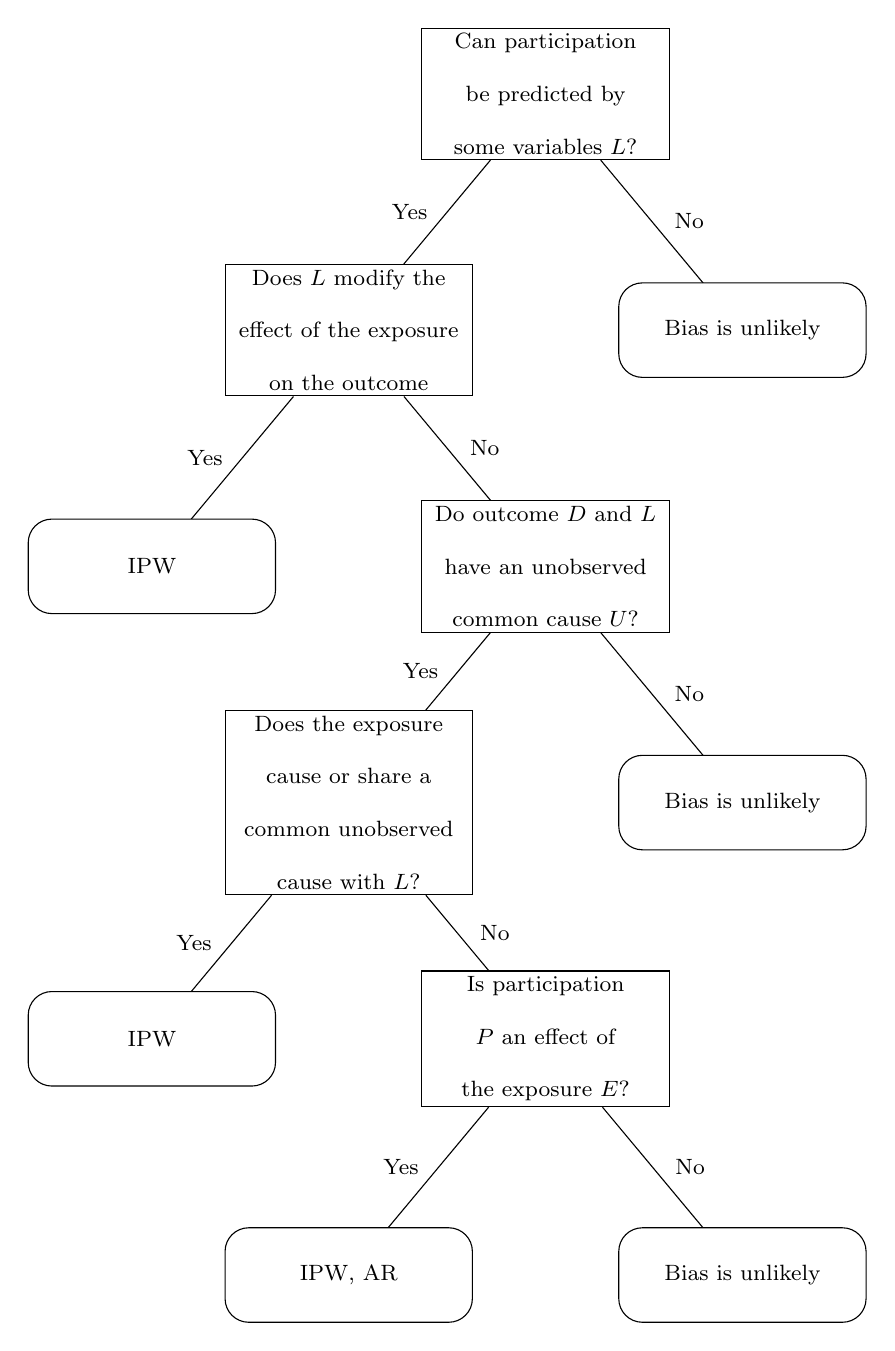
\begin{tikzpicture}
	[
	 sibling distance = 4cm,
	 level distance   = 3cm,
	 every node/.style = {shape=rectangle,
		                  draw,
		                  align=center,
		                  top color = white,
	                      font=\footnotesize,
	                      minimum size = 12mm,
	                      text width = 30mm,
	                      inner sep = 2pt
                         },
    L1/.style = {sibling distance=9cm},
    L2/.style = {sibling distance=5cm},
    L3/.style = {sibling distance=1cm},
    YN/.style = {minimum size = 8mm,
    	         text width = 8mm,
    	         pos = .5,
    	         text opacity = 1,
    	         fill opacity=0}
	]
	
	\newcommand{\LP}{Can participation be predicted by some variables $L$?}
	\newcommand{\nB}{Bias is unlikely}
	\newcommand{\LED}{Does $L$ modify the effect of the exposure
		on the outcome }
	\newcommand{\EL}{Does the exposure cause
		or share a common unobserved
		cause with $L$?}
	\newcommand{\EP}{Is participation $P$
		an effect of
		the exposure $E$?}
	\newcommand{\CCDL}{Do outcome $D$ and $L$
		have an unobserved
		common cause $U$?}	

	\node (A) {\LP}
	child [L2] {[] node  (B1) {\LED}
				child [L2] {[rounded corners=3mm] node (C1) {IPW}}
			    child [L2] {[] node (C2) {\CCDL}
		                    child [L2] {[] node (D1) {\EL}
		                    	        child [L2] {[rounded corners=3mm] node (E1) {IPW}}
		                    	        child [L2] {[] node (E2) {\EP}
		                    	        	        child [L2] {[rounded corners=3mm] node (F1) {IPW, AR}}
		                    	        	        child [L2] {[rounded corners=3mm] node (F2) {\nB}}
		                    	                                      }
		                                                  }
		                    child [L2] {[rounded corners=3mm] node (D2) {\nB}}                    
	                                         }}
	child [L2] {[rounded corners=3mm] node  (B2) {\nB}};
	
	 \begin{scope}[nodes = {draw = none}]
	   \path (A)  -- (B1) node [YN, left]   {Yes};
	   \path (A)  -- (B2) node [YN, right]  {No};
	   \path (B1) -- (C1) node [YN, left]   {Yes};
	   \path (B1) -- (C2) node [YN, right]  {No};
	   \path (C2) -- (D1) node [YN, left]   {Yes};
	   \path (C2) -- (D2) node [YN, right]  {No};
	   \path (D1) -- (E1) node [YN, left]   {Yes};
	   \path (D1) -- (E2) node [YN, right]  {No};
	   \path (E2) -- (F1) node [YN, left]   {Yes};
	   \path (E2) -- (F2) node [YN, right]  {No};
	 \end{scope}
\end{tikzpicture}}	
    \end{singlespace}
	
	%
\begin{tikzpicture}
	[
	 sibling distance = 4cm,
	 level distance   = 4cm,
	 every node/.style = {shape=rectangle,
		                  draw,
		                  align=center,
		                  top color = white,
	                      font=\footnotesize,
	                      minimum size = 22mm,
	                      text width = 28mm,
	                      inner sep = 0pt
                         },
    L1/.style ={sibling distance=9cm},
    L2/.style ={sibling distance=5cm},
    L3/.style ={sibling distance=3cm},
    YN/.style = {minimum size = 8mm,
    	text width = 8mm,
    	pos = .5,
    	text opacity = 1,
    	fill opacity=0}
	]
	
	\newcommand{\LP}{Is there a participation indicator $L$?}
	\newcommand{\nB}{Bias is unlikely}
	\newcommand{\LED}{Does $L$ modify the effect of the exposure
		             on the outcome }
	\newcommand{\EL}{Does the expo- sure cause
		             or share a common unobserved
		             cause with $L$?}
    \newcommand{\EP}{Is participation $P$
    	             an effect of
    	             the exposure $E$?}
    \newcommand{\CCDL}{Do outcome $D$ and $L$
    	               have an unobserved
    	               common cause $U$?}	
	\node (A) {\LP}
	child [L2] {[] node  (B1) {\LED}
				child [L1] {[] node (C1) {\EP}
					        child [L2] {[] node (Dx1) {\EL}
					        	        child [L2] {[] node (Ex1) {\CCDL}
					        	        	        child [L2] {[rounded corners=3mm] node (Fx1) {IPPW}}
					        	        	        child [L2] {[rounded corners=3mm] node (Fx2) {DS/MRP, IPPW}}
					        	                                         }
					        	        child [L2] {[rounded corners=3mm] node (Ex2) {DS/MRP, IPPW}}
					                                       }
					        child [L2] {[rounded corners=3mm] node (Dx2) {DS/MRP, IPPW}}
				                              }
			    child [L1] {[] node (C2) {\CCDL}
		                    child [L2] {[] node (D1) {\EL}
		                    	        child [L2] {[rounded corners=3mm] node (E1) {IPPW}}
		                    	        child [L2] {[] node (E2) {\EP}
		                    	        	        child [L2] {[rounded corners=3mm] node (F1) {AR, DS/MRP, IPPW}}
		                    	        	        child [L2] {[rounded corners=3mm] node (F2) {\nB}}
		                    	                                      }
		                                                  }
		                    child [L2] {[rounded corners=3mm] node (D2) {\nB}}                    
	                                         }}
	child [L2] {[rounded corners=3mm] node  (B2) {\nB}};
	
	 \begin{scope}[nodes = {draw = none}]
	   \path (A)  -- (B1) node [YN, left]   {Yes};
	   \path (A)  -- (B2) node [YN, right]  {No};
	   \path (B1) -- (C1) node [YN, left]   {Yes};
	   \path (B1) -- (C2) node [YN, right]  {No};
	   \path (C2) -- (D1) node [YN, left]   {Yes};
	   \path (C2) -- (D2) node [YN, right]  {No};
	   \path (D1) -- (E1) node [YN, left]   {Yes};
	   \path (D1) -- (E2) node [YN, right]  {No};
	   \path (E2) -- (F1) node [YN, left]   {Yes};
	   \path (E2) -- (F2) node [YN, right]  {No};
	   \path (Dx1) -- (Ex1) node [YN, left]   {Yes};
	   \path (Dx1) -- (Ex2) node [YN, right]  {No};
	   \path (C1) -- (Dx1) node [YN, left]   {Yes};
	   \path (C1) -- (Dx2) node [YN, right]  {No};
	   \path (Ex1) -- (Fx1) node [YN, left]   {Yes};
	   \path (Ex1) -- (Fx2) node [YN, right]  {No};
	 \end{scope}
\end{tikzpicture}
	\caption{Decision tree for identification of selection bias and choice of approach to correct it. See Figure \ref{fig:SelectionBias} for causal diagrams that underlie the decision tree. 
	To determine if selection bias is likely, and if so which correction method can be used, proceed through the questions from the top on. Ending in a node "Bias is unlikely" implies that an  analysis without correction for selection bias will still result in estimates without selection bias. Otherwise, different correction types can be used, depending on the underlying causal structure. IPPW stands for analysis with inverse probability of participation weighting, AR for adjusted regression. For reasons of brevity, this decision tree does not isolate cases where multilevel regression and post stratification (MRP) can be used to correct bias.}
	\label{fig:DecisionTree}
\end{figure}


Structural analysis using directed acyclic graphs (DAGs) is a useful tool for the development of analysis strategies that remains underused. A practical argument against the use of DAGs is the uncertainty about hypothesised causal relationships. We proposed to use genetic correlation coefficients from LD score regression of publicly available GWAS summary statistics as one possibility to substantiate central assumptions about unobserved common causes. The main motivation to focus on common genetic causes is the growing availability of GWAS summary statistics and methodological advances allowing estimation of heritability and genetic correlation coefficients from such statistics \cite{Bulik-Sullivan2015-er, Bulik-Sullivan2015-xn}. Because GWAS studies are association studies, they do not provide unambiguous proof for a causal role of genes. Even if GWAS associations estimates are partly driven by environmental factors, genetic correlation estimates from GWAS summary statistics are of interest, because common environmental causes also contribute to the manifestation of selection bias. If direct estimates of common environmental causes are available, they should also be used for evaluating DAGs. Last but not least, the analysis of implied conditional independencies of competing causal models also allows examination of hypothesized causal relationships. As described in the supplementary discussion, such an analysis shows that the data analysed here are not consistent with a causal model in which exposure and participation predictors are independent in the target population (c.f. \ref{fig:SelectionBias}).

A second challenge when using structural models is the difficulty of formulating DAGs for complex causal models \cite{Shrier2008-vr}. When judging the presence of bias due to self-selection and selective dropout, a simple decision tree can supplant the formulation of a complete DAG, so that researchers can determine the potential for selection bias by answering a sequence of questions about the relationship of participation predictors, exposures, and outcomes. Figure \ref{fig:DecisionTree} shows a decision tree that identifies when correction for bias is necessary, and what correction method is appropriate.

A topic closely related to selection bias is that of representativeness. While it was argued that representativeness can be detrimental to scientific inference, because understanding of mechanisms and careful control of relevant variables are central for this aim \cite{Rothman2013-qc}, others have emphasised the importance of representativeness---understood as the availability of weights for calculating valid population estimates \cite{Keiding2016-fv}. Careful experimentation based on hypothesised mechanisms is undoubtedly central to scientific progress. Still, this approach does not describe the often-exploratory analyses of cohort study data well. Moreover, if one understands causal inference as the central goal of scientific inquiry, ignoring non-representativeness of unweighted study samples does not only undermine generalization to the population of interest, but can also lead to incorrect scientific inferences by facilitating the "discovery" of associations where there are in fact none, or prevent the detection of existing associations.

In conclusion, self-selection into cohort studies and loss to follow-up can lead to biased estimates of exposure-outcome associations from large population based cohort studies. Structural analysis and empirical results suggest that especially for mental health related exposures and outcomes selection bias is likely. Still, the dependency of bias on the specific outcome, exposure, and study participation predictors makes general statements about selection bias for multi-exposure multi-outcome studies impossible. Instead, each  investigation of an exposure-outcome association has to assess selection bias. If bias is likely and valid participation predictors are available, weighting study participants by the inverse of their participation probability is a robust approach to control bias due to self-selection and loss to follow-up.


\vspace{3cm}

Funding: This study was funded by the Norwegian Institute of Public Health.


Conflict of Interest: The authors declare that they have no conflict of interest.


\newpage

\printbibliography

\newpage

\processdelayedfloats

\clearpage

\makeatletter
\efloat@restorefloats
\makeatother

\appendix

\renewcommand{\thefigure}{S\arabic{figure}}
\renewcommand{\thepostfigure}{S\arabic{postfigure}}
\setcounter{figure}{0}
\setcounter{postfigure}{0}

\renewcommand{\thetable}{S\arabic{table}}
\renewcommand{\theposttable}{S\arabic{posttable}}
\setcounter{table}{0}
\setcounter{posttable}{0}

%\begin{comment}

\phantomsection{Supplementary Information}
\setcounter{page}{1}

%\phantomsection{Supplementary tables}

\begin{table}
	\caption{}
	\label{tab:regmodels}
\end{table}

\begin{table}
	\caption{}
	\label{tab:gwas}
\end{table}

\begin{table}
	\caption{}
	\label{tab:rg}
\end{table}

\begin{table}
	\caption{}
	\label{tab:estimates-UR}
\end{table}

%\phantomsection{Supplementary figures}

\begin{figure}
	\caption{}
	\label{fig:prop_moba_ssb}
\end{figure}

\begin{figure}
	\caption{}
	\label{fig:coverage}
\end{figure}

\begin{figure}
	\caption{}
	\label{fig:ADHDsumscore}
\end{figure}

\begin{figure}
	\caption{}
	\label{fig:covariation}
\end{figure}

\begin{figure}
	\caption{}
	\label{fig:IPW}
\end{figure}

\begin{figure}
	\caption{}
	\label{fig:IPWbalance}
\end{figure}

\begin{figure}
	\caption{}
	\label{fig:logRRsAR}
\end{figure}

\begin{figure}
	\caption{}
	\label{fig:logRRsUR}
\end{figure}

\begin{figure}
	\caption{}
	\label{fig:ropeplotsAR}
\end{figure}

\begin{figure}
	\caption{}
	\label{fig:ropeplotsUR}
\end{figure}

%\end{comment}

\end{document}
